\chapter{Network evaluation} %%%%%%%%%%%%%%%%%%%%%%%%%%%%%%%%%%%%%%%%%%%%%%%%%%%%%%%%%%%%%%%%%%%%%
\label{chap:results} %%%%%%%%%%%%%%%%%%%%%%%%%%%%%%%%%%%%%%%%%%%%%%%%%%%%%%%%%%%%%%%%%%%%%%%%%%%%%

This chapter provides a comprehensive evaluation of how the new CNN approach behaves. Four
categories of understanding are explored (each a section of this chapter):
\begin{enumerate}
    \item determining the beam selection and energy estimation performance;
    \item explaining the inner workings of the trained networks;
    \item studying how robust the network outputs are to changes in the input; and
    \item exploring alternative implementations to see which factors drive performance.
\end{enumerate}

Beforehand, a hugely impactful advantage of the CNN approach must be highlighted. Although the
time taken to train the CNNs in this work is approximately two days, once trained the time
required to calculate all network outputs (inference time) for a single event is on the order of
\unit{2}{\text{ms}}. When combined with event seeding and event map generation, the total time
taken to fully reconstruct and classify a raw event is less than \unit{0.1}{\text{seconds}}.
Compared to the $\sim$\unit{15}{\text{minutes}} required for each event using the standard
reconstruction and classification methods (with multiple hypotheses), the difference is stark.

Armed with this incredible speed, the time taken to fully process a large dataset containing
millions of events becomes a matter of hours, compared to the many weeks typically required. This
change has far-reaching implications for how physics analysis is conducted. By removing the
processing bottleneck, larger datasets can be used without worry, new techniques can be tested
quickly, and overall analysis turnover increased.

\section{Performance} %%%%%%%%%%%%%%%%%%%%%%%%%%%%%%%%%%%%%%%%%%%%%%%%%%%%%%%%%%%%%%%%%%%%%%%%%%%%
\label{sec:results_eval} %%%%%%%%%%%%%%%%%%%%%%%%%%%%%%%%%%%%%%%%%%%%%%%%%%%%%%%%%%%%%%%%%%%%%%%%%

Here the performance of the CNN approach is presented and compared to that achieved by the
standard \chips methods as well as comparable experiments. Primarily this focuses on the principal
aim of selecting an efficient and pure appeared CC $\nu_{e}$ signal sample with accurate neutrino
energy estimation. However, the survived CC $\nu_{\mu}$ selection is also presented for
completeness.

\subsection{Evaluation sample and preselection} %%%%%%%%%%%%%%%%%%%%%%%%%%%%%%%%%%%%%%%%%%%%%%%%%%
\label{sec:results_eval_sample} %%%%%%%%%%%%%%%%%%%%%%%%%%%%%%%%%%%%%%%%%%%%%%%%%%%%%%%%%%%%%%%%%%

An independent sample of events is used to evaluate the combined performance of the trained CNNs.
The evaluation sample consists of 400000 beam and 350000 cosmic muon events produced in the same
way as the training and validation events, using the detector simulation and event generation
methods outlined in \SectionRef{sec:chips_monte_carlo}. The beam events include the expected
$\nu_{\mu}$, $\bar{\nu}_{\mu}$, $\nu_{e}$ and $\bar{\nu}_{e}$ components as well as events
generated to mimic the appeared (sometimes referred to as \emph{App}) $\nu_{e}$ component. Only
the neutrino mode (forward horn current) of NuMI beam operation is considered here. During the
evaluation, the intrinsic neutrino and antineutrino components of the beam are considered the same
for simplicity.

All evaluation events are weighted to match the expected spectrum at the \chipsfive detector using
the unoscillated flux, cross-sections, and oscillation probabilities (including the MSW effect).
Additional weighting also scales the sample to match data taking in the NuMI beam for a single
year, corresponding to $6\times 10^{20}$ protons on target (POT). Cosmic muon events are weighted
according to the \unit{11.8}{\text{kHz}} expected \chipsfive rate outlined in
\SectionRef{sec:chips_monte_carlo_cosmic}. The final weighted spectrum of events is shown in
\FigureRef{fig:explore_osc_fluxes} with the combination of underlying beam neutrino interaction
types shown in \FigureRef{fig:explore_stacked_int_types}.

\begin{figure} % OSC FLUXES DIAGRAM %
    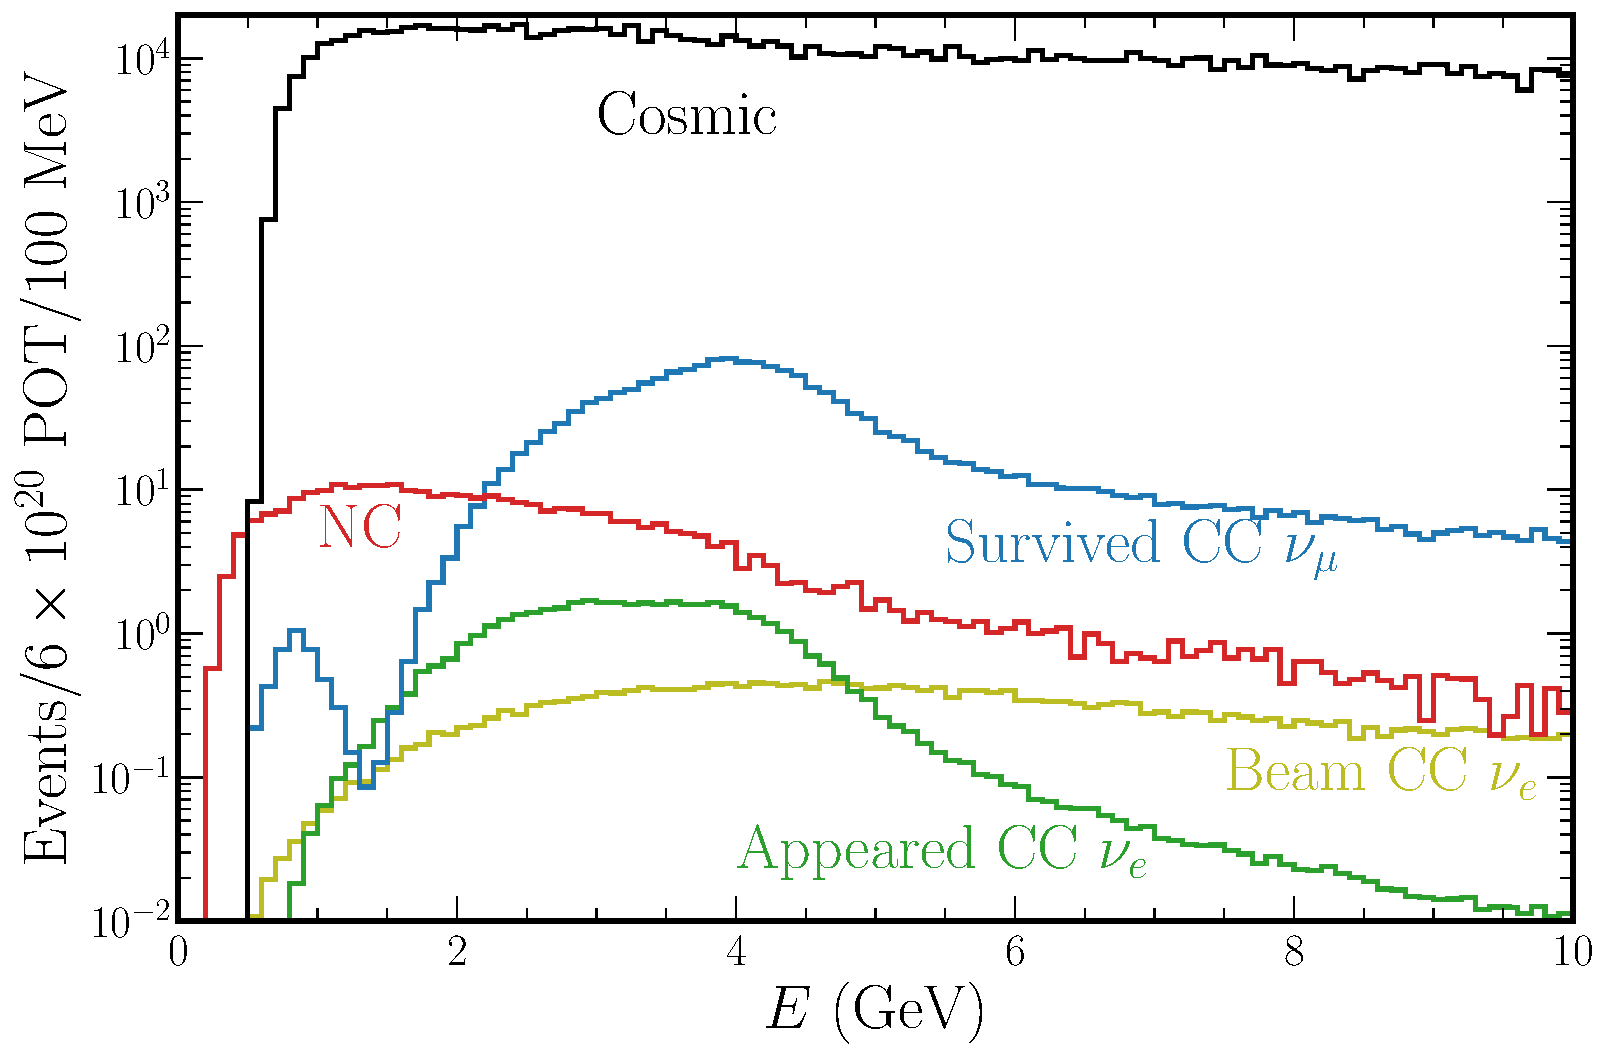
\includegraphics[width=0.7\textwidth]{diagrams/7-results/explore_osc_fluxes.pdf}
    \caption[Weighted spectrum of evaluation sample events]
    {Weighted spectrum of events contained within the evaluation sample. The weighting is designed
        to mimic the expected event spectrum of the \chipsfive detector. Beam events are weighted
        by combining the expected unoscillated flux with cross-sections and standard oscillation
        probabilities, while cosmic events are weighted using the expected cosmic rate. Shown in
        blue, green, and olive are the surviving CC $\nu_{\mu}$, appearing CC $\nu_{e}$, and
        intrinsic beam CC $\nu_{e}$ spectra respectively, binned in terms of their neutrino
        energy. Shown in red is the NC event spectra, binned in terms of the energy of the
        hadronic component (excluding the outgoing neutrino energy) to represent more accurately
        the energy visible to the detector. Finally, shown in black is the cosmic muon event
        spectra binned in terms of the muon energy.}
    \label{fig:explore_osc_fluxes}
\end{figure}

\begin{figure} % STACK INT TYPES DIAGRAM %
    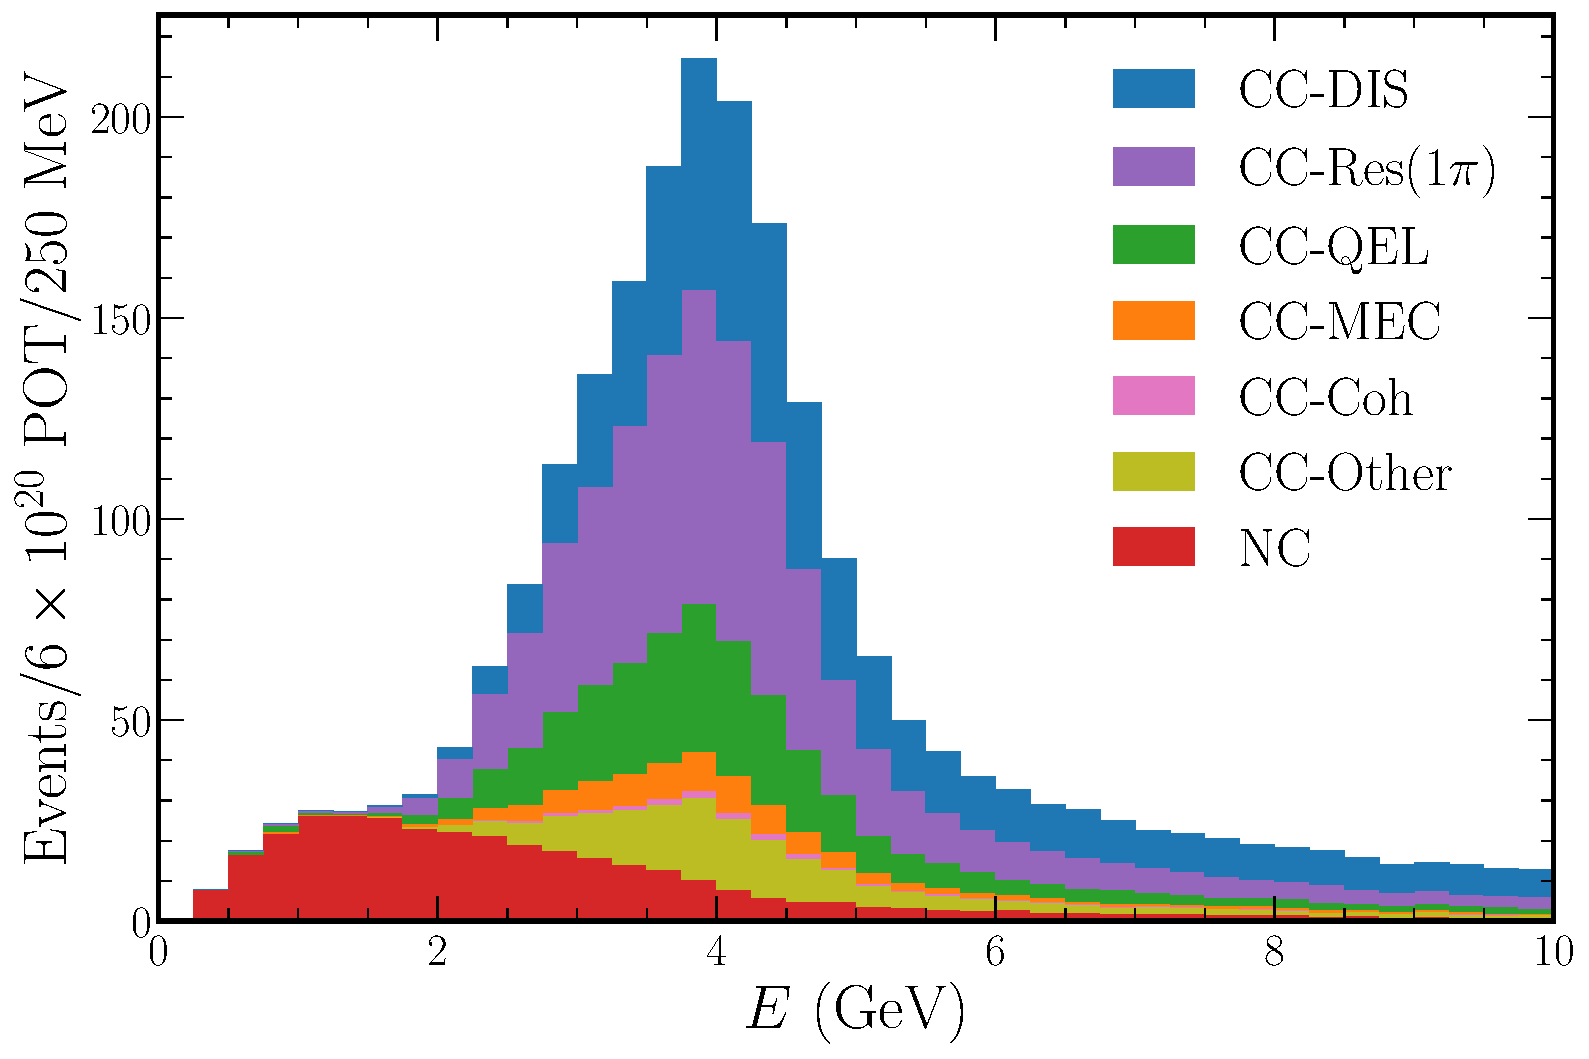
\includegraphics[width=0.7\textwidth]{diagrams/7-results/explore_stacked_int_types.pdf}
    \caption[Weighted spectrum of interaction types within the evaluation sample]
    {Weighted spectrum of $\nu_{\mu}$ and $\nu_{e}$ beam events contained within the evaluation
        sample separated by interaction type. CC events are binned in terms of neutrino energy
        while NC events are binned in terms of the hadronic component energy.}
    \label{fig:explore_stacked_int_types}
\end{figure}

Separate from the CNN driven work, a simple preselection is applied to all evaluation sample
events. Designed to reject cosmic and NC events while keeping the efficiency of CC beam events
high, the preselection consists of four simple cuts, shown in \FigureRef{fig:explore_simple_cuts}.
Firstly, the total number of collected photoelectrons (charge) across all PMTs in the event must
be greater than 250. Secondly, the maximum Hough transform space height must be greater than 250
photoelectrons. Thirdly, the seeding procedure $\cos(\theta)$ direction must be between $\pm$0.7.
Finally, the seeding procedure $\phi$ direction must be between $\pm$1.1 radians. The first two
cuts reject low energy events which are usually NC in nature, while the last two reject events
whose activity is not along the beamline, typically cosmic.

\begin{figure} % SIMPLE CUTS DIAGRAM %
    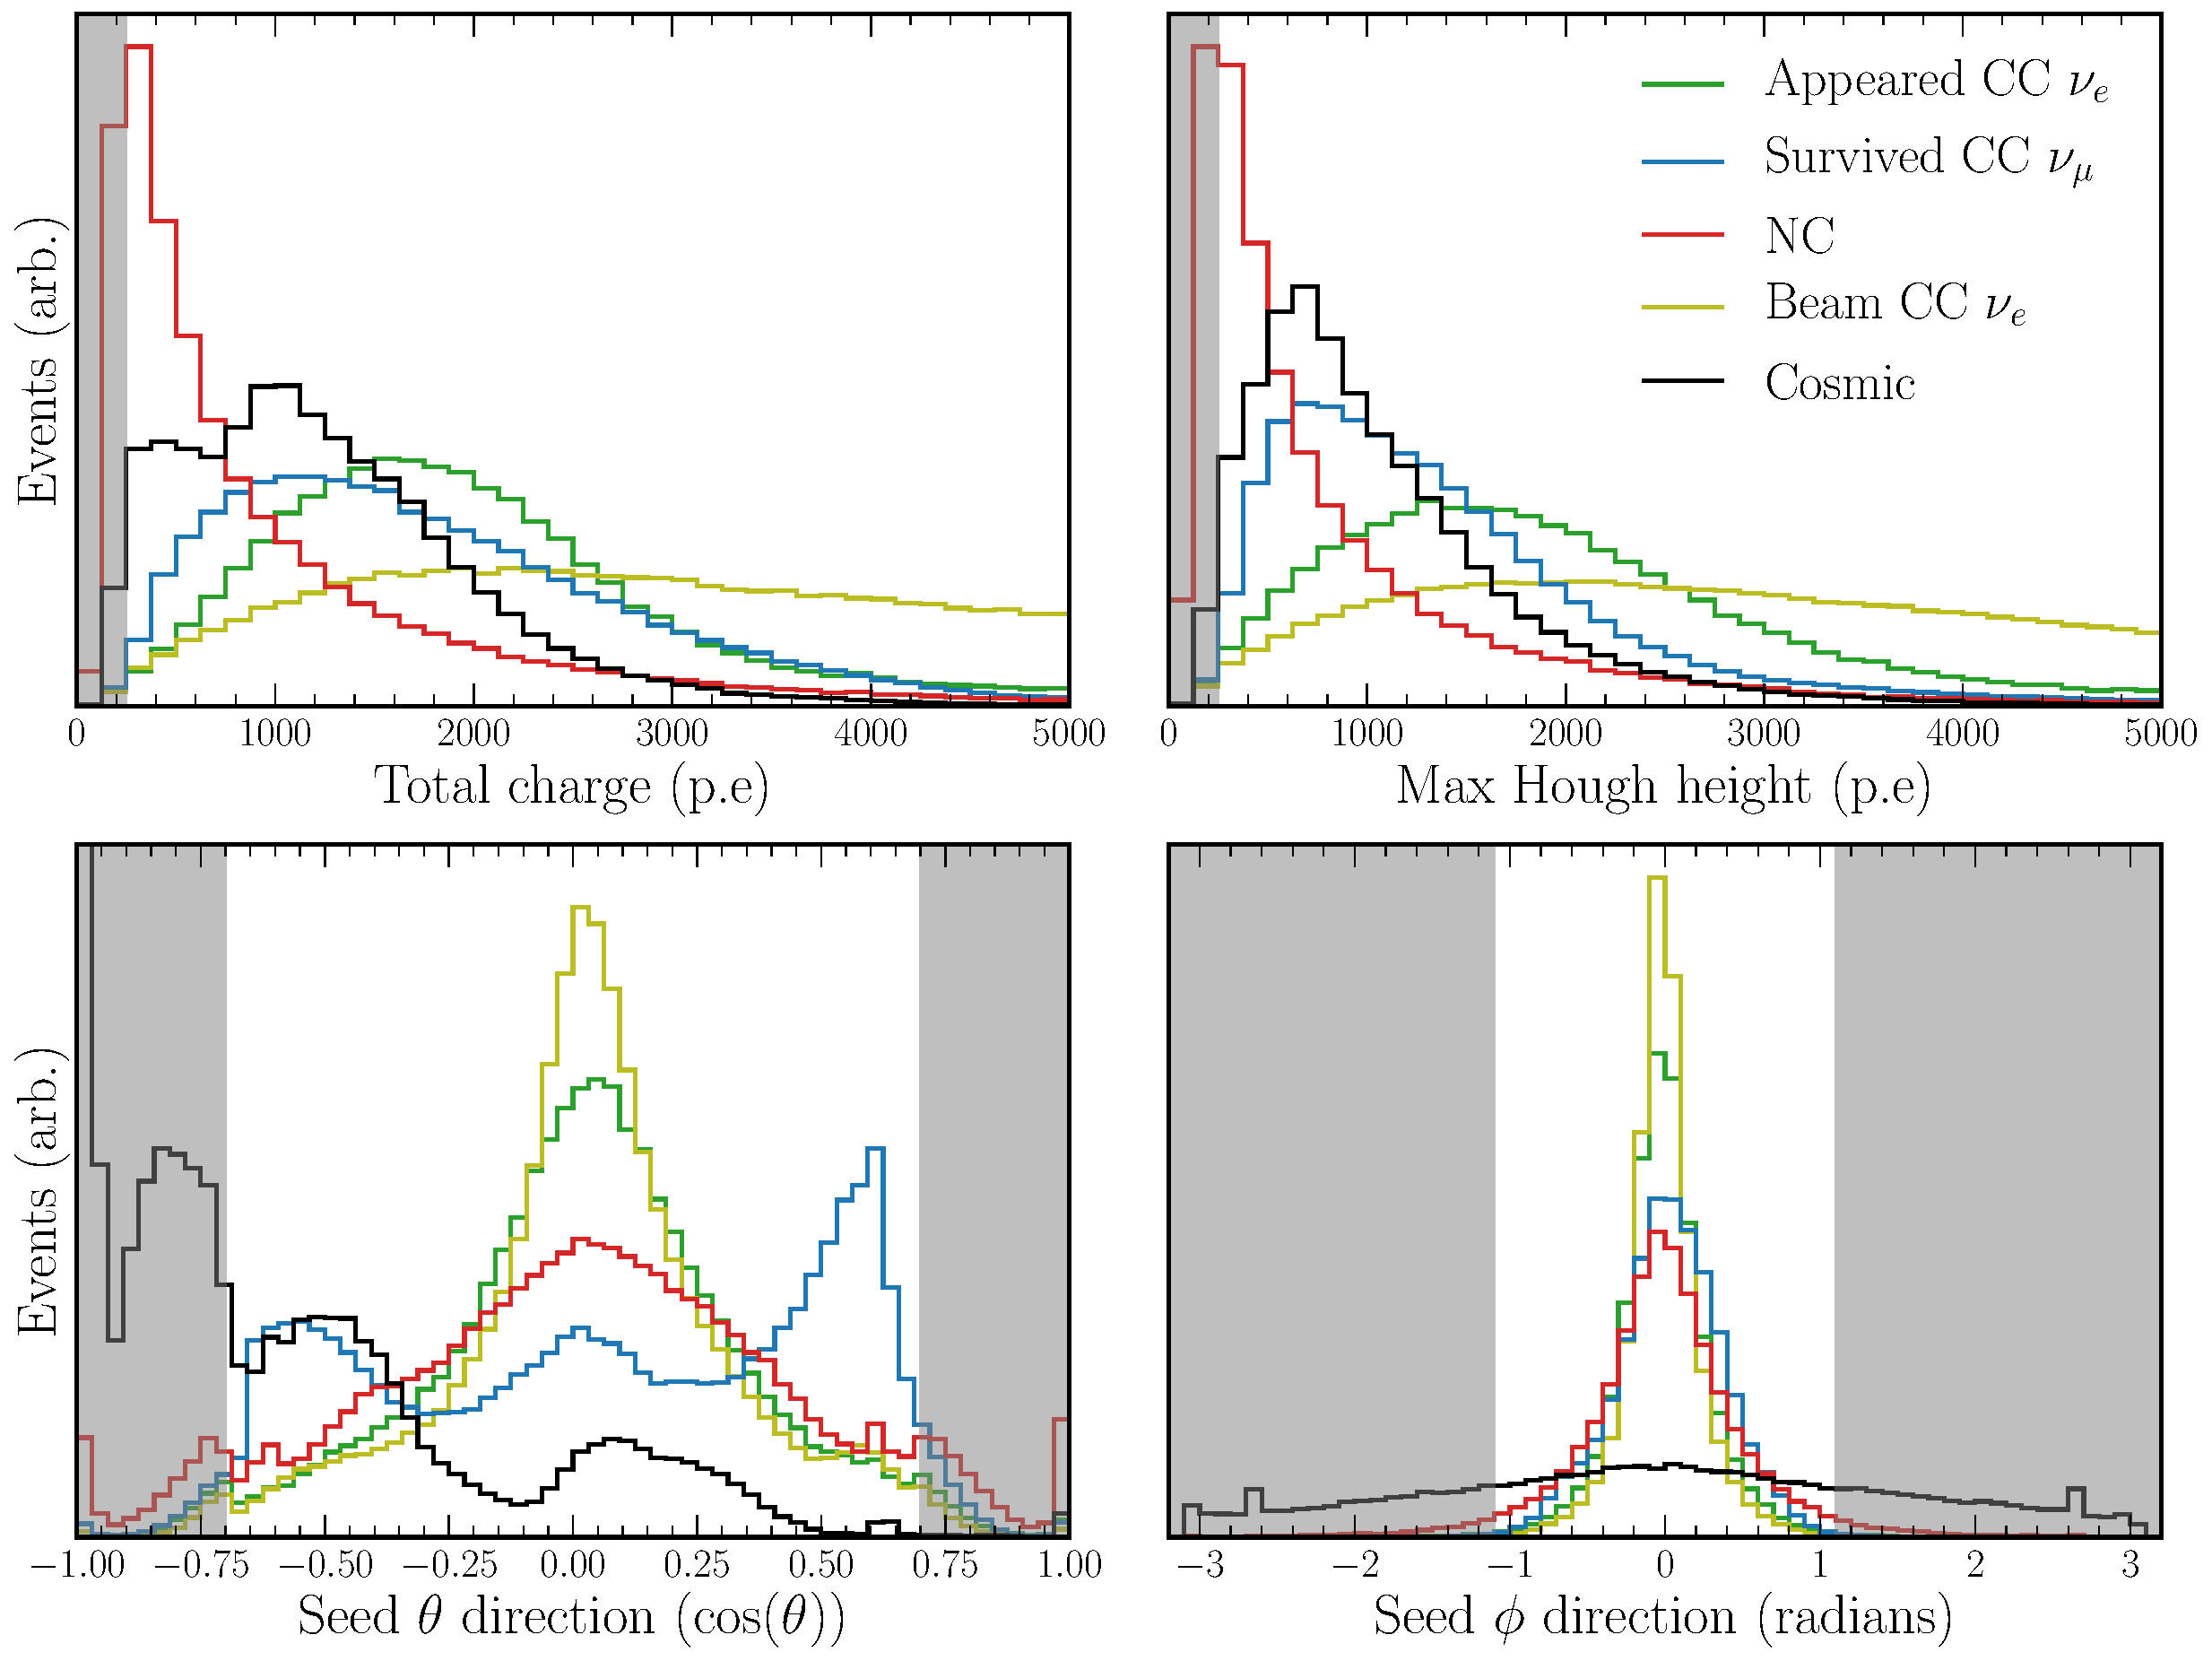
\includegraphics[width=\textwidth]{diagrams/7-results/explore_simple_cuts.pdf}
    \caption[Plots detailing evaluation sample preselection cuts]
    {Plots showing the four preselection cuts and how they affect the different event categories.
        The grey regions indicate rejected events.}
    \label{fig:explore_simple_cuts}
\end{figure}

\subsection{Cosmic rejection and containment} %%%%%%%%%%%%%%%%%%%%%%%%%%%%%%%%%%%%%%%%%%%%%%%%%%%%
\label{sec:results_eval_cosmic} %%%%%%%%%%%%%%%%%%%%%%%%%%%%%%%%%%%%%%%%%%%%%%%%%%%%%%%%%%%%%%%%%%

\subsubsection*{Cosmic score} %%%%%%%%%%%%%%%%%%%%%%%%%%%%%%%%%%%%%%%%%%%%%%%%%%%%%%%%%%%%%%%%%%%%

The \emph{cosmic score} output from the trained cosmic rejection network shows an excellent
separation between beam (output close to zero) and cosmic (output close to one) events, as can be
seen in \FigureRef{fig:cosmic_outputs}. Notably, the vast majority of beam events are associated
with a score incredibly close to zero as is more clearly shown in
\FigureRef{fig:cosmic_zoomed_outputs}. Given this fact, a tight \emph{cosmic score} cut of below
$0.0001$ is chosen by inspection to select beam like events. Out of the total $350000$ cosmic
events in the evaluation sample, all are rejected by this cut alongside preselection.

\begin{figure} % COSMIC OUTPUTS DIAGRAM %
    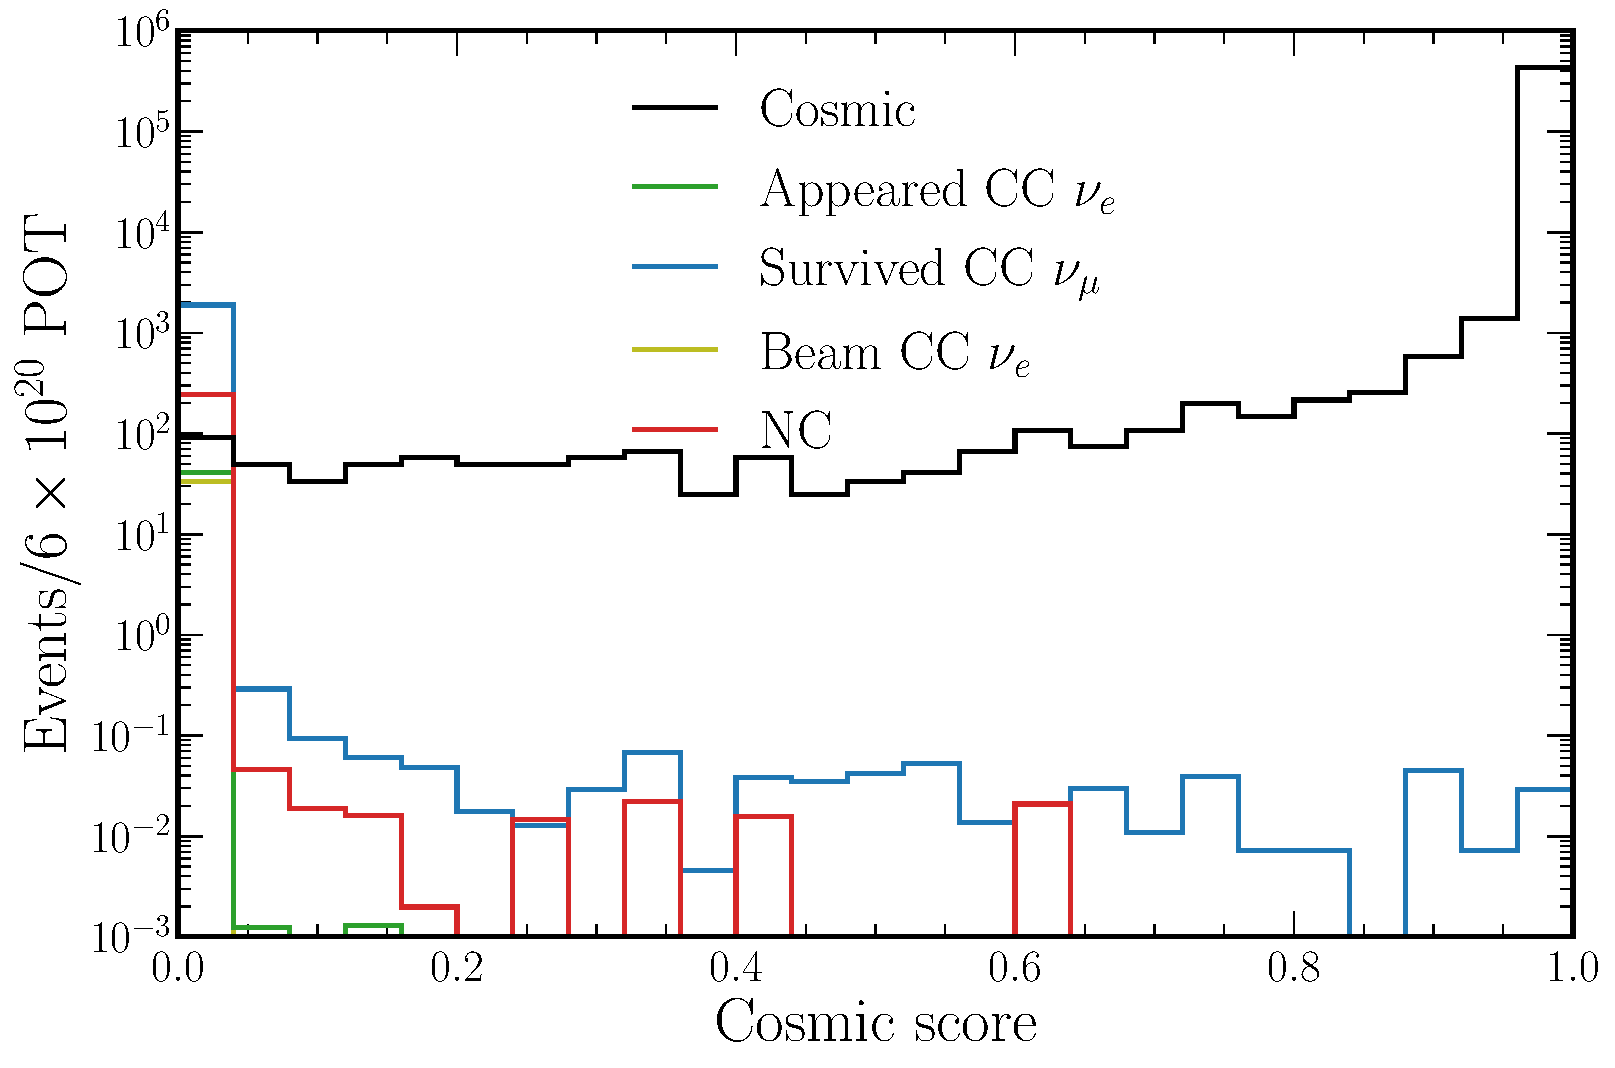
\includegraphics[width=0.7\textwidth]{diagrams/7-results/final_cosmic_outputs.pdf}
    \caption[Distribution of cosmic score output values]
    {Distribution of \emph{cosmic score} output values from the trained cosmic rejection network
        for the different event categories. A score close to one signifies a cosmic like event,
        while a score close to zero corresponds to a beam like event. Only preselected events are
        shown to better highlight the events this output aims to classify.}
    \label{fig:cosmic_outputs}
\end{figure}

\begin{figure} % COSMIC OUTPUTS ZOOMED DIAGRAM %
    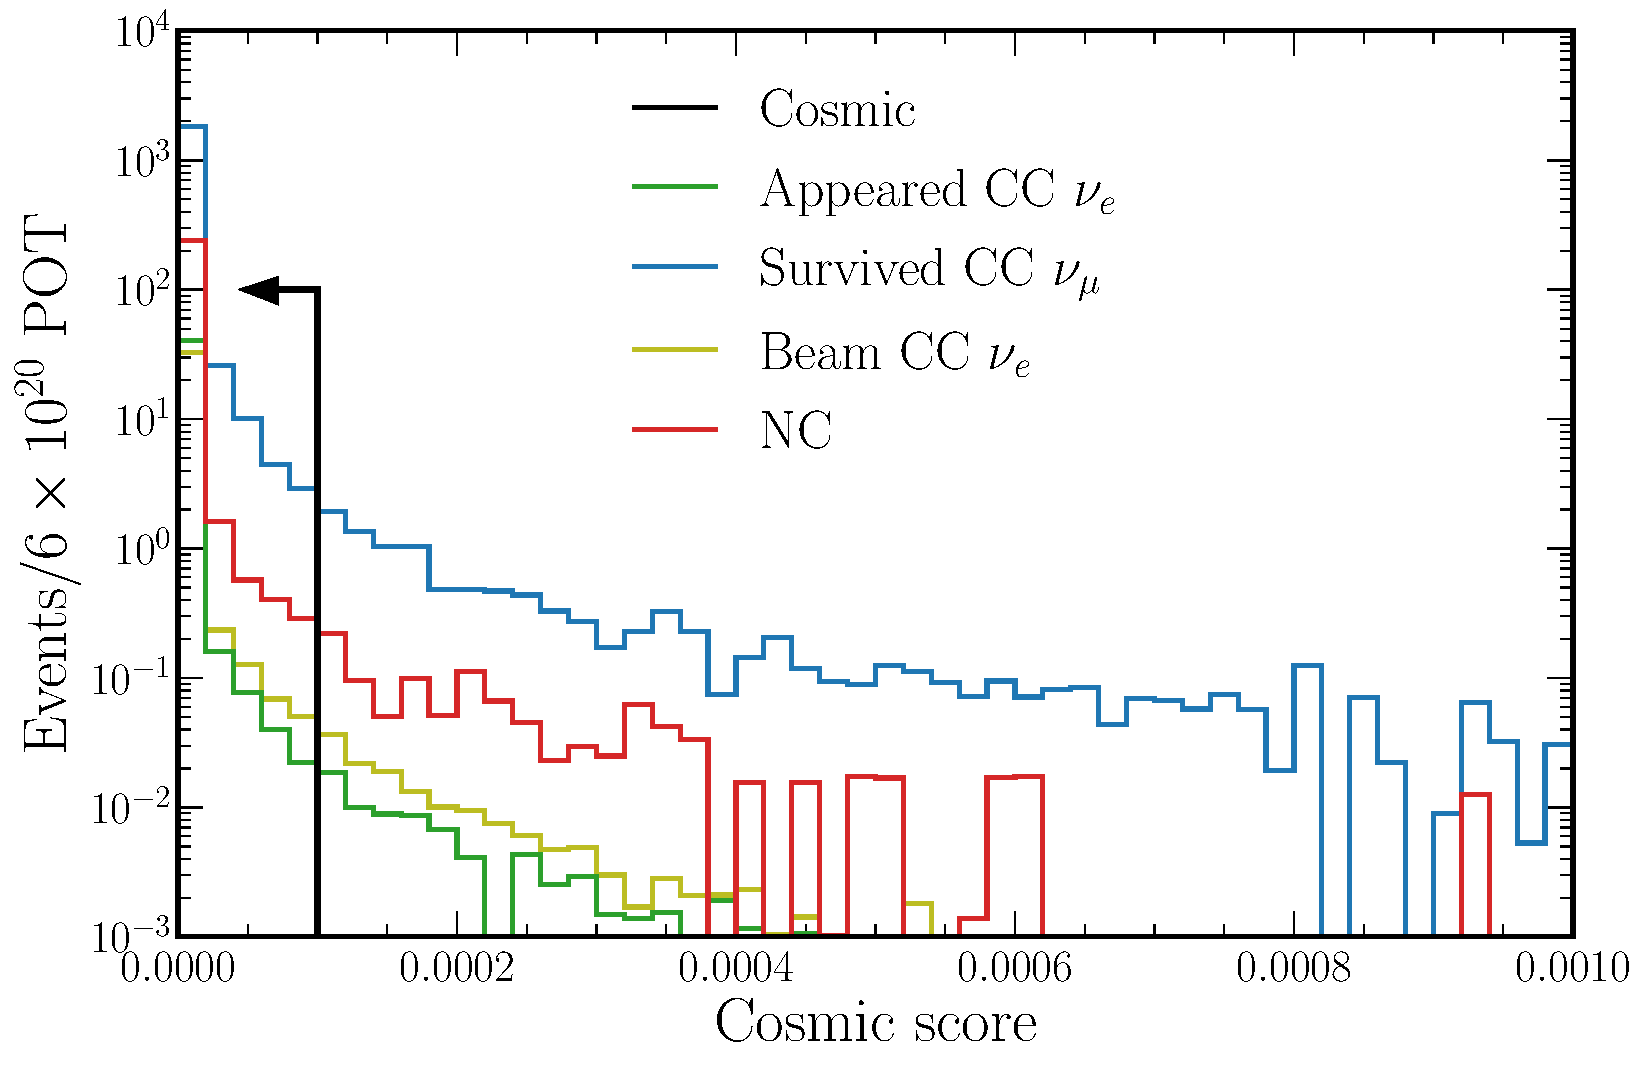
\includegraphics[width=0.7\textwidth]{diagrams/7-results/final_cosmic_zoomed_outputs.pdf}
    \caption[Distribution of cosmic score output values close to zero]
    {Distribution of \emph{cosmic score} output values from the trained cosmic rejection network
        close to zero for the different event categories. The cosmic rejection cut value at 0.0001
        is shown with the arrow indicating selected events. No cosmic events are within the shown
        range due to the statistical limitations of the evaluation sample.}
    \label{fig:cosmic_zoomed_outputs}
\end{figure}

\subsubsection*{Escapes score} %%%%%%%%%%%%%%%%%%%%%%%%%%%%%%%%%%%%%%%%%%%%%%%%%%%%%%%%%%%%%%%%%%%

It is crucial for accurate neutrino energy estimation that the activity of an event is fully
contained within the volume of the detector. If charged event particles instead leave the detector
and emit Cherenkov radiation not captured by PMTs, it can be incredibly difficult to estimate the
resulting missing energy and hence neutrino energy. Within the \chipsfive detector, this is
particularly important for long track CC $\nu_{\mu}$ events for which only 44\% of the primary
charged muons are fully contained within the detector volume.

Therefore, the second output from the cosmic rejection network, \emph{escapes score} is also used
to select events. Although this output only considers the primary charged lepton, instead of all
event particles, it still acts as a reasonable proxy for event containment. The distribution of
\emph{escapes score} output values for each event category is shown in
\FigureRef{fig:final_escapes_outputs}.

An \emph{escapes score} value below 0.5 is chosen to select events for which the primary charged
lepton is fully contained within the detector. With this selection, 97\% and 96\% of CC
$\nu_{\mu}$ events for which the primary charged lepton is contained within or escapes the
detector respectively are classified correctly. For the selected CC $\nu_{\mu}$ events this
corresponds to a 95\% purity. As expected, the vast majority of CC $\nu_{e}$ and NC events are
selected.

For comparison with other experiments, the escapes cut effectively works as a quasi fiducial
volume cut, for an energy-dependent region near the downstream wall of the detector. Fiducial
volume cuts are common in HEP experiments to remove events whose activity is close to the detector
walls and, therefore, can not be reconstructed well. Future work should explore how a fully
implemented fiducial cut using the reconstructed interaction vertex position, impacts performance.

\begin{figure} % ESCAPES OUTPUTS DIAGRAM %
    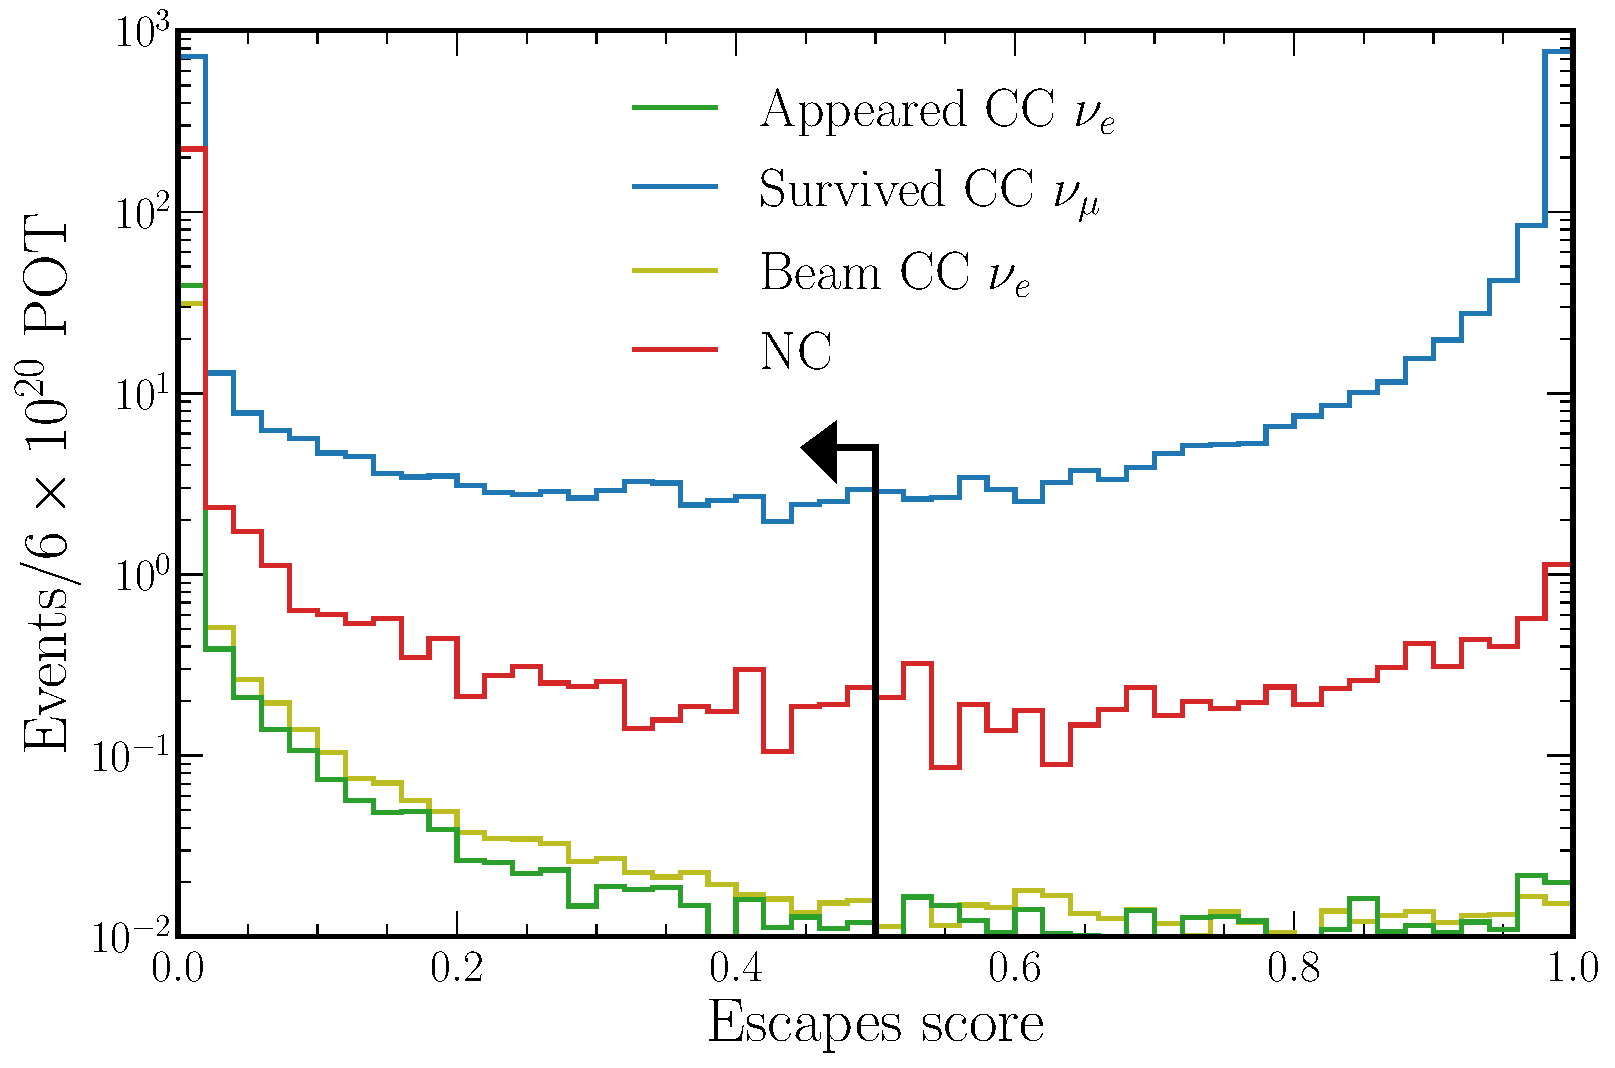
\includegraphics[width=0.7\textwidth]{diagrams/7-results/final_escapes_outputs.pdf}
    \caption[Distribution of escapes score output values]
    {Distribution of \emph{escapes score} output values from the trained cosmic rejection network
        for the different event categories. A score close to one signifies an escaped primary
        charged lepton like event, while a score close to zero corresponds to a contained primary
        charged lepton like event. The containment cut value at 0.5 is shown with the arrow
        indicating the events that are selected.}
    \label{fig:final_escapes_outputs}
\end{figure}

\subsubsection*{Combined rejection} %%%%%%%%%%%%%%%%%%%%%%%%%%%%%%%%%%%%%%%%%%%%%%%%%%%%%%%%%%%%%%

The total number of expected events per year that pass each successive cut (including
preselection) for each event category is shown in \TableRef{tab:selection}. Both CC $\nu_{e}$
categories are selected with an efficiency greater than 90\%, while CC $\nu_{\mu}$ events are
reduced to a 40\% efficiency, mainly by the \emph{escapes score} cut, to ensure they are fully
contained. Furthermore, NC events are found to be primarily rejected by the preselection, while
cosmic events are heavily rejected by both the preselection and \emph{cosmic score} cuts.

\begin{table}
    \begin{tabular}{lrrrrr}
                       & App CC $\nu_{e}$ & CC $\nu_{\mu}$ & Beam CC $\nu_{e}$ & NC             &
                       Cosmic                 \\
        \midrule
        Total events   & 44.2             & 2045.9         & 35.1              & 348.7          &
        1211000                \\
        + preselection & 41.2             & 1889.5         & 33.5              & 239.6          &
        249260                 \\
        + cosmic cut   & 41.1             & 1874.4         & 33.4              & 238.0          &
        0.13                   \\
        + escapes cut  & 40.8             & 818.0          & 33.0              & 231.0          &
        0.02                   \\
        \midrule
        Efficiency     & $92.4\pm0.4\%$   & $40.0\pm0.2\%$ & $94.2\pm0.4\%$    & $66.3\pm0.7\%$ &
        $\sim1.5\times10^{-8}$ \\
    \end{tabular}
    \caption[Number of events passing successive selection cuts for each event category]
    {The total number of expected (weighted) events and the number that pass successive selection
        cuts for the different event categories. The preselection, \emph{cosmic score} cut, and
        \emph{escapes score} cut numbers are shown. The selection efficiency after all cuts have
        been applied is also shown for each event category.}
    \label{tab:selection}
\end{table}

When compared to the approximately 2.1 million expected cosmic events per year, the zero selected
out of 350000 evaluation events is not statistically significant. However, the generation of a
sufficiently sized cosmic evaluation sample is deemed infeasible due to the vast computational
resources required.

Therefore, to more accurately gauge the number of cosmic events likely to be classified as beam
events, we consider the more statistically significant number that passes a loose \emph{cosmic
score} cut below a value of $0.9$. In this case, when combined with the preselection and
\emph{escapes score} cut, $38$ out of $350000$ evaluation sample cosmic events are selected, which
when weighted gives $317$ events per year. Assuming a flat distribution of events between a
\emph{cosmic score} of $0.0$ and $0.9$, and using the actual $0.0001$ cut value, $0.035$ events
are expected to be selected. This number corresponds to an excellent cosmic muon rejection factor
of $\sim1.5\times10^{-8}$.

Additionally, of the $317$ events under a \emph{cosmic score} value of $0.9$, $167$ would be
selected as CC $\nu_{\mu}$ and zero as CC $\nu_{e}$ by the beam classification detailed in
\SectionRef{sec:results_eval_beam}. Therefore, even if a tiny number of cosmic events are
selected, they would likely be classified as CC $\nu_{\mu}$ events, not contaminating the
principal CC $\nu_{e}$ selection. In summary, the expected cosmic muon contamination of both beam
selections is expected to be negligible and ignored for the rest of this performance evaluation.

\subsection{Beam classification} %%%%%%%%%%%%%%%%%%%%%%%%%%%%%%%%%%%%%%%%%%%%%%%%%%%%%%%%%%%%%%%%%
\label{sec:results_eval_beam} %%%%%%%%%%%%%%%%%%%%%%%%%%%%%%%%%%%%%%%%%%%%%%%%%%%%%%%%%%%%%%%%%%%%

The output values from each of the \emph{combined category} neurons of the trained beam
classification network give the probability score that an event belongs to the corresponding
category. As the neuron output scores collectively sum to one, the highest-scoring neuron can be
used to classify events as either CC $\nu_{e}$, CC $\nu_{\mu}$, or NC in nature.
\FigureRef{fig:final_comb_cat_confusion} shows the resulting classification matrix using this
approach.

\begin{figure} % FINAL COMB CAT CONFUSION DIAGRAM %
    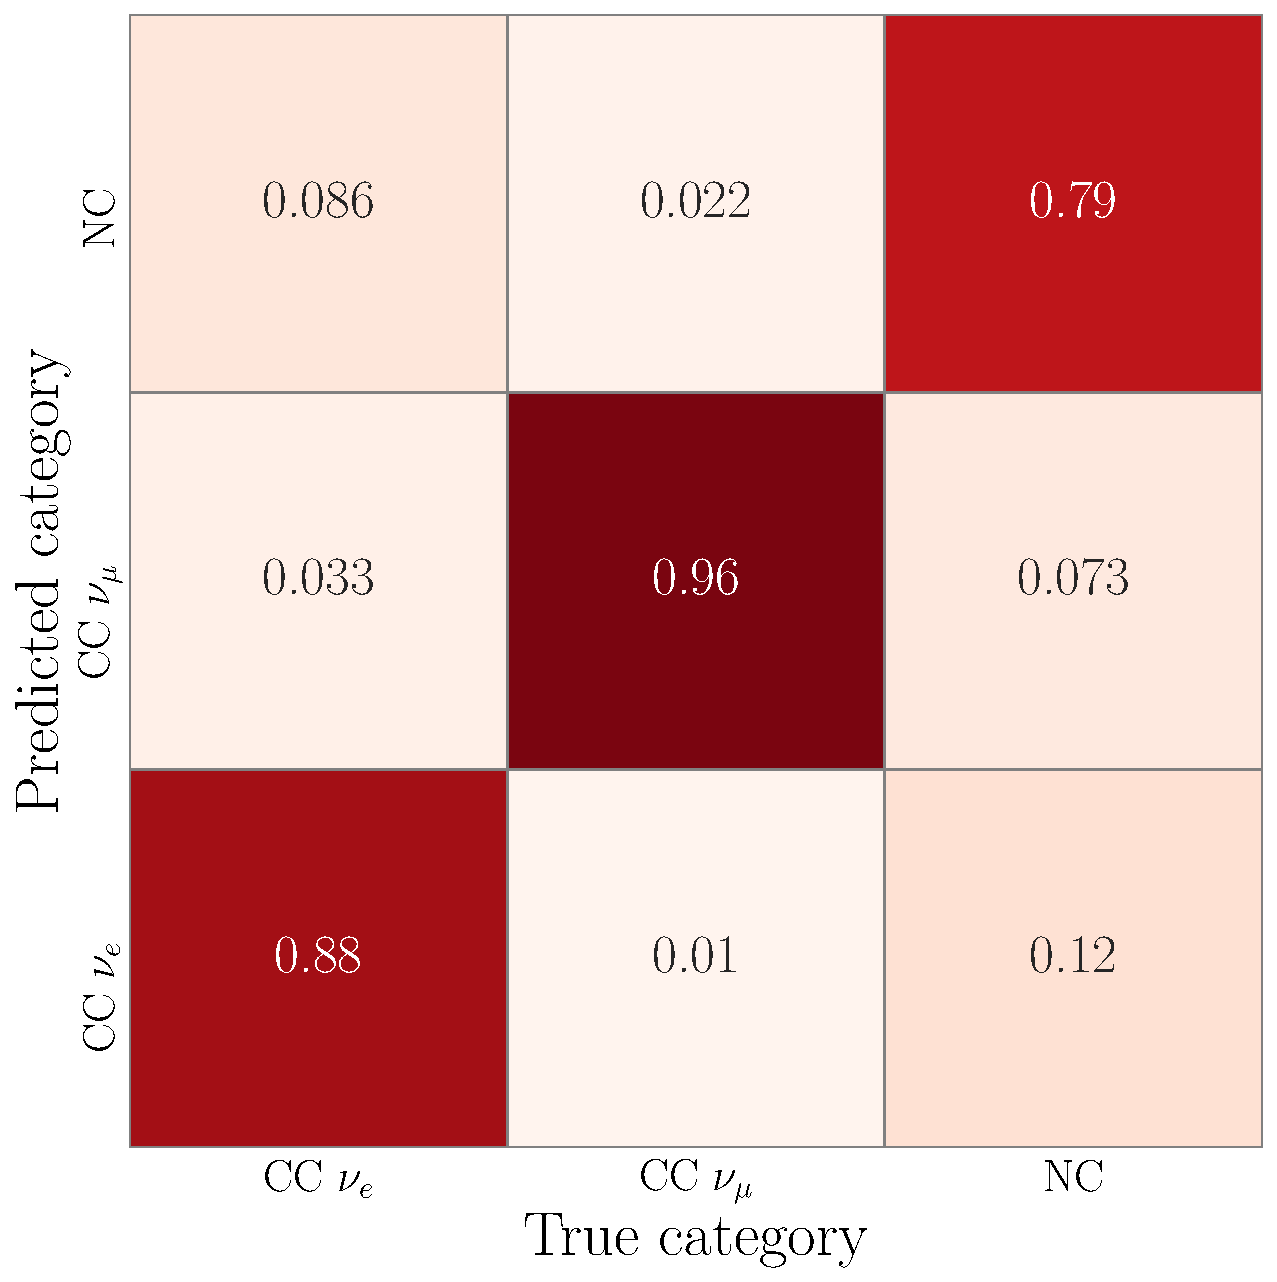
\includegraphics[width=0.6\textwidth]{diagrams/7-results/final_comb_cat_confusion.pdf}
    \caption[Classification matrix for the combined category output of the beam classification
        network] {Classification matrix for the \emph{combined category} output of the trained
        beam classification network. Events are simply classified using the categorical score for
        which they have the highest value. The numbers shown are the fraction of true category
        events classified into each of the three possible categories.}
    \label{fig:final_comb_cat_confusion}
\end{figure}

To access the beam classification performance more rigorously, a selection score for each of the
output categories, found by maximising a figure-of-merit (FOM), is instead calculated. All events
with a score above this optimised value are then deemed signal. To minimise the expected
measurement statistical error, the value of $\text{efficiency}\times\text{purity}$ (proportional
to $s/\sqrt{s+b}$) is optimised as the FOM~\cite{list2002}. Below, the results for both appeared
CC $\nu_{e}$ and survived CC $\nu_{\mu}$ selections using this methodology are presented.

\subsubsection*{CC $\nu_{e}$ selection} %%%%%%%%%%%%%%%%%%%%%%%%%%%%%%%%%%%%%%%%%%%%%%%%%%%%%%%%%%

The distribution of CC $\nu_{e}$ scores for the different event categories are shown in
\FigureRef{fig:final_beam_nuel_outputs}. A strong separation between appeared CC $\nu_{e}$ signal
and both CC $\nu_{\mu}$ and NC background events is achieved. As no attempt is made to separate
the appeared CC $\nu_{e}$ signal component from the intrinsic beam CC $\nu_{e}$ background, both
are clustered with scores close to one as expected.

\begin{figure} % BEAM OUTPUTS NUEL DIAGRAM %
    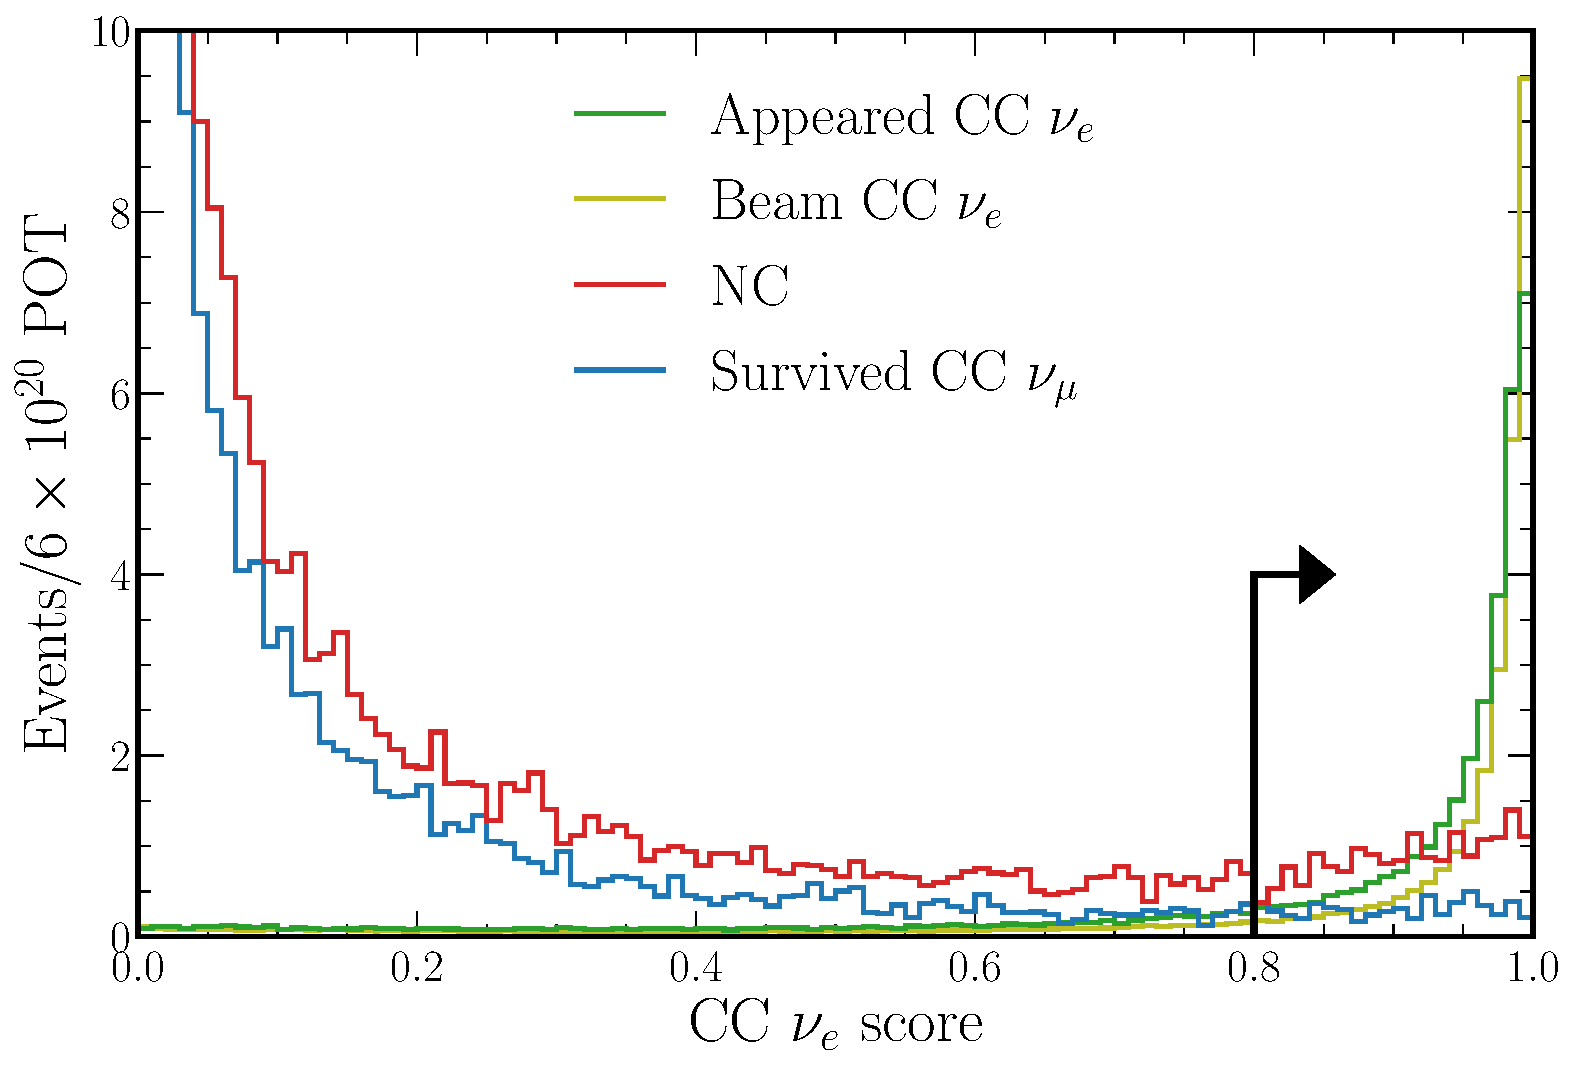
\includegraphics[width=0.7\textwidth]{diagrams/7-results/final_beam_nuel_outputs.pdf}
    \caption[Distribution of CC $\nu_{e}$ scores from the trained beam classification network]
    {Distribution of \emph{combined category} CC $\nu_{e}$ scores from the trained beam
        classification network for the different event categories. A score close to one signifies
        a CC $\nu_{e}$ like event. The y-axis has been truncated so that the CC $\nu_{\mu}$ and NC
        components are not fully visible to better show the distribution of signal CC $\nu_{e}$
        events.}
    \label{fig:final_beam_nuel_outputs}
\end{figure}

The efficiency, purity, and their product (the FOM) for CC $\nu_{e}$ events (both appeared and
beam) as a function of selecting events above a certain CC $\nu_{e}$ score are shown in
\FigureRef{fig:final_nuel_eff_curves}. $\text{Efficiency}\times\text{purity}$ is optimised by
selecting events with a CC $\nu_{e}$ score above $0.8$, achieving a value of $0.519$. Note that
$\text{efficiency}\times\text{purity}$ is optimised considering both appeared and beam CC
$\nu_{e}$ components as signal due to their indistinguishable nature.

The corresponding number and efficiency of selected events for each event category, as well as the
appeared signal CC $\nu_{e}$ purity, are shown in \TableRef{tab:nuel_selection}. The final FOM
selected signal purity of $38.3\pm0.5\%$ may appear low, but this is mainly due to the
indistinguishable intrinsic beam CC $\nu_{e}$ contamination. When both CC $\nu_{e}$ components are
considered signal, the selection purity becomes $71.0\pm0.6\%$.

\begin{figure} % FINAL NUEL EFF CURVES DIAGRAM %
    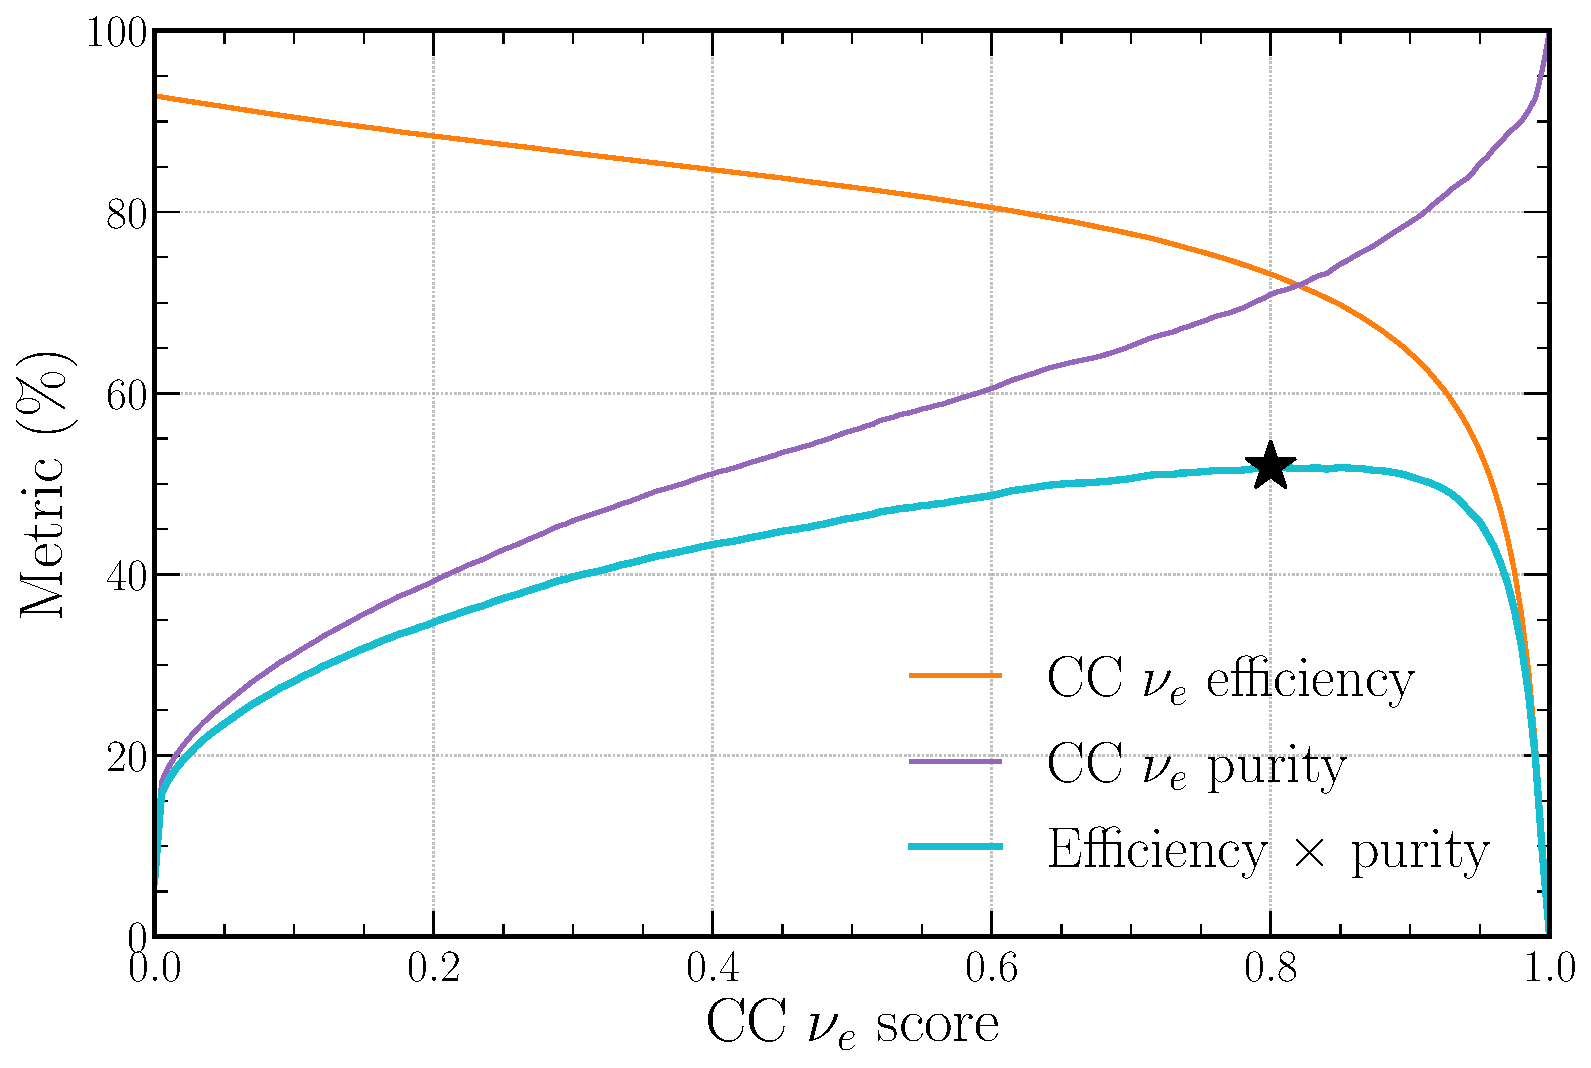
\includegraphics[width=0.7\textwidth]{diagrams/7-results/final_nuel_eff_curves.pdf}
    \caption[CC $\nu_{e}$ efficiency, purity, and $\text{efficiency}\times\text{purity}$ curves]
    {CC $\nu_{e}$ efficiency, purity, and $\text{efficiency}\times\text{purity}$ curves for
        different values of CC $\nu_{e}$ score selection.}
    \label{fig:final_nuel_eff_curves}
\end{figure}

\begin{table}
    \begin{tabular}{lrrrrr}
                 & CC $\nu_{e}$ sig & Beam CC $\nu_{\mu}$ bkg & CC $\nu_{e}$ bkg & NC bkg        &
                 Sig Purity     \\
        \midrule
        Cuts Num & 40.8             & 818.0                   & 33.0             & 231.0         &
        $3.6\pm0.1\%$  \\
        FOM Num  & 31.3             & 6.1                     & 26.7             & 17.6          &
        $38.3\pm0.5\%$ \\
        \midrule
        FOM Eff  & $70.9\pm0.4\%$   & $0.3\pm0.02\%$          & $76.3\pm0.3\%$   & $5.1\pm0.2\%$ &
        -              \\
    \end{tabular}
    \caption[Table showing CC $\nu_{e}$ selected event numbers, efficiencies and signal purity]
    {Table showing CC $\nu_{e}$ selected event numbers and corresponding efficiencies for the
        various event categories as well as the associated signal purity. Shown are the numbers
        for both the post preselection, \emph{cosmic score} cut, and \emph{escapes score} cut
        numbers (Cuts) in addition to the numbers after the       
        $\text{efficiency}\times\text{purity}$ (FOM) optimised selection for which the efficiency
        is shown.}
    \label{tab:nuel_selection}
\end{table}

The $\text{efficiency}\times\text{purity}$ optimised CC $\nu_{e}$ selection efficiency as a
function of energy for the different event categories is shown in
\FigureRef{fig:final_nuel_hists}. From low neutrino energies, both CC $\nu_{e}$ category selection
efficiencies rise steeply to a plateau of approximately 80\% beginning at \unit{4}{GeV}. This is
expected as low energy CC $\nu_{e}$ events have less well-defined electron Cherenkov rings,
leading to their rejection. Due to the abundance of selected intrinsic beam CC $\nu_{e}$ events at
higher energies, the appeared CC $\nu_{e}$ purity is observed to peak at approximately
\unit{2.5}{\GeV} (reasonably close to the oscillation maximum) before declining. The NC efficiency
is seen to slowly increase, approaching 15\% for hadronic component energies above \unit{5}{\GeV};
this is likely due to misidentification of high energy pions or protons as electrons. Importantly,
however, within the key signal region from 2 to \unit{4}{\GeV}, NC selection efficiency remains
low.

\begin{figure} % FINAL NUEL HISTS DIAGRAM %
    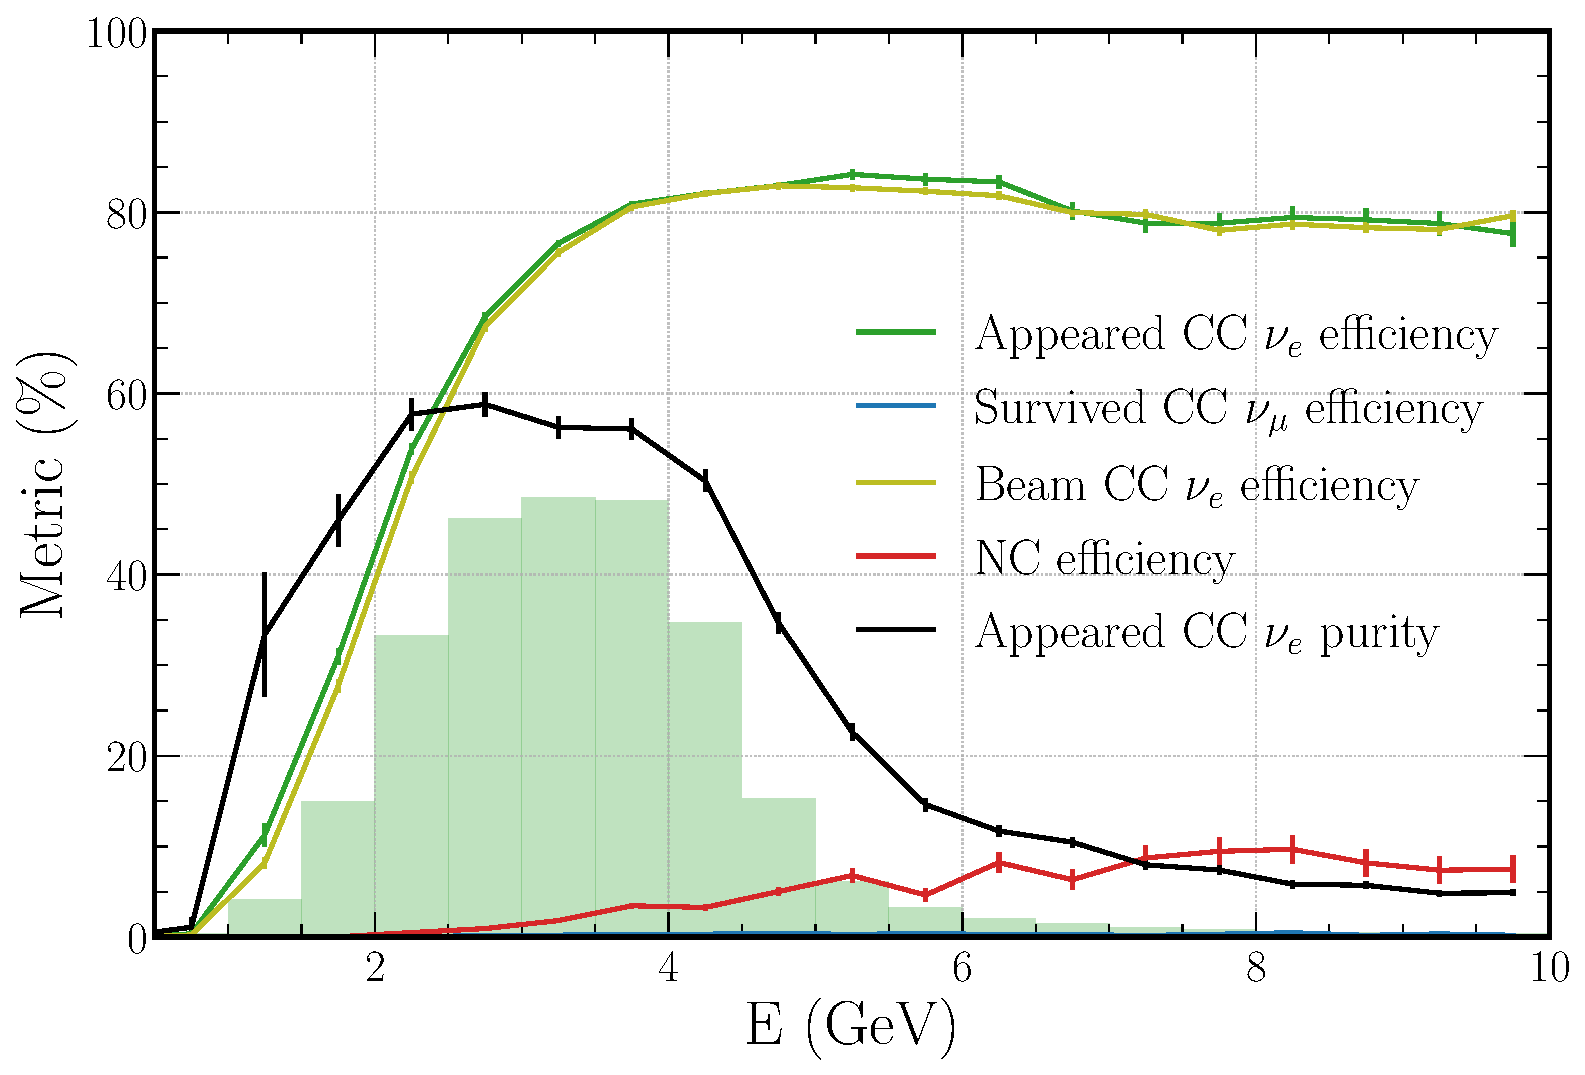
\includegraphics[width=0.7\textwidth]{diagrams/7-results/final_nuel_hists.pdf}
    \caption[Efficiency of the CC $\nu_{e}$ selection as a function of energy]
    {Efficiency of the CC $\nu_{e}$ selection for the different event categories as well as
        appeared CC $\nu_{e}$ purity as a function of energy. All CC categories are shown in terms
        of neutrino energy, while NC events are shown in terms of the hadronic component energy.
        The survived CC $\nu_{\mu}$ efficiency is so low it is barely visible near zero. For
        reference, the true appeared CC $\nu_{e}$ neutrino energy distribution is shown in the
        green.}
    \label{fig:final_nuel_hists}
\end{figure}

The best way to understand the relative performance of the CNN CC $\nu_{e}$ classification is by
comparison with the standard event selection presented in \SectionRef{sec:cnn_old_pid}. The
distribution of output scores from both simple neural networks used in the standard selection are
shown in \FigureRef{fig:final_old_pid_outputs}. By optimising the selection values for both
networks, 0.91 and 0.78 respectively, to maximise $\text{efficiency}\times\text{purity}$, the
standard CC $\nu_{e}$ selected sample is found. All events that pass the preselection, not just
those shown in \FigureRef{fig:final_old_pid_outputs} are used in this optimisation.

A maximum $\text{efficiency}\times\text{purity}$ of 0.132 is achieved; only 25\% the value reached
by the CNN approach. Both the combined appeared and beam CC $\nu_{e}$ efficiency of 34\% compared
to 71\% and purity of 39\% compared to 71\% are considerably lower than that provided by the new
CNN classification.

Furthermore, the new signal efficiency of 71\% compares well to the 62\% and 64\% achieved by the
\nova and T2K CC $\nu_{e}$ selections, respectively. However, purity is significantly lower at
38\% compared to the 78\% and 80\% reached by \nova and T2K~\cite{acero2019, abe2015}. A large
proportion of this difference can be explained by the lower neutrino energies at which these
experiments operate. Not only does this increase the proportion of easy to identify CC-QEL events,
but also lowers the indistinguishable intrinsic beam CC $\nu_{e}$ contamination.

\begin{figure} % FINAL OLD PID OUTPUTS DIAGRAM %
    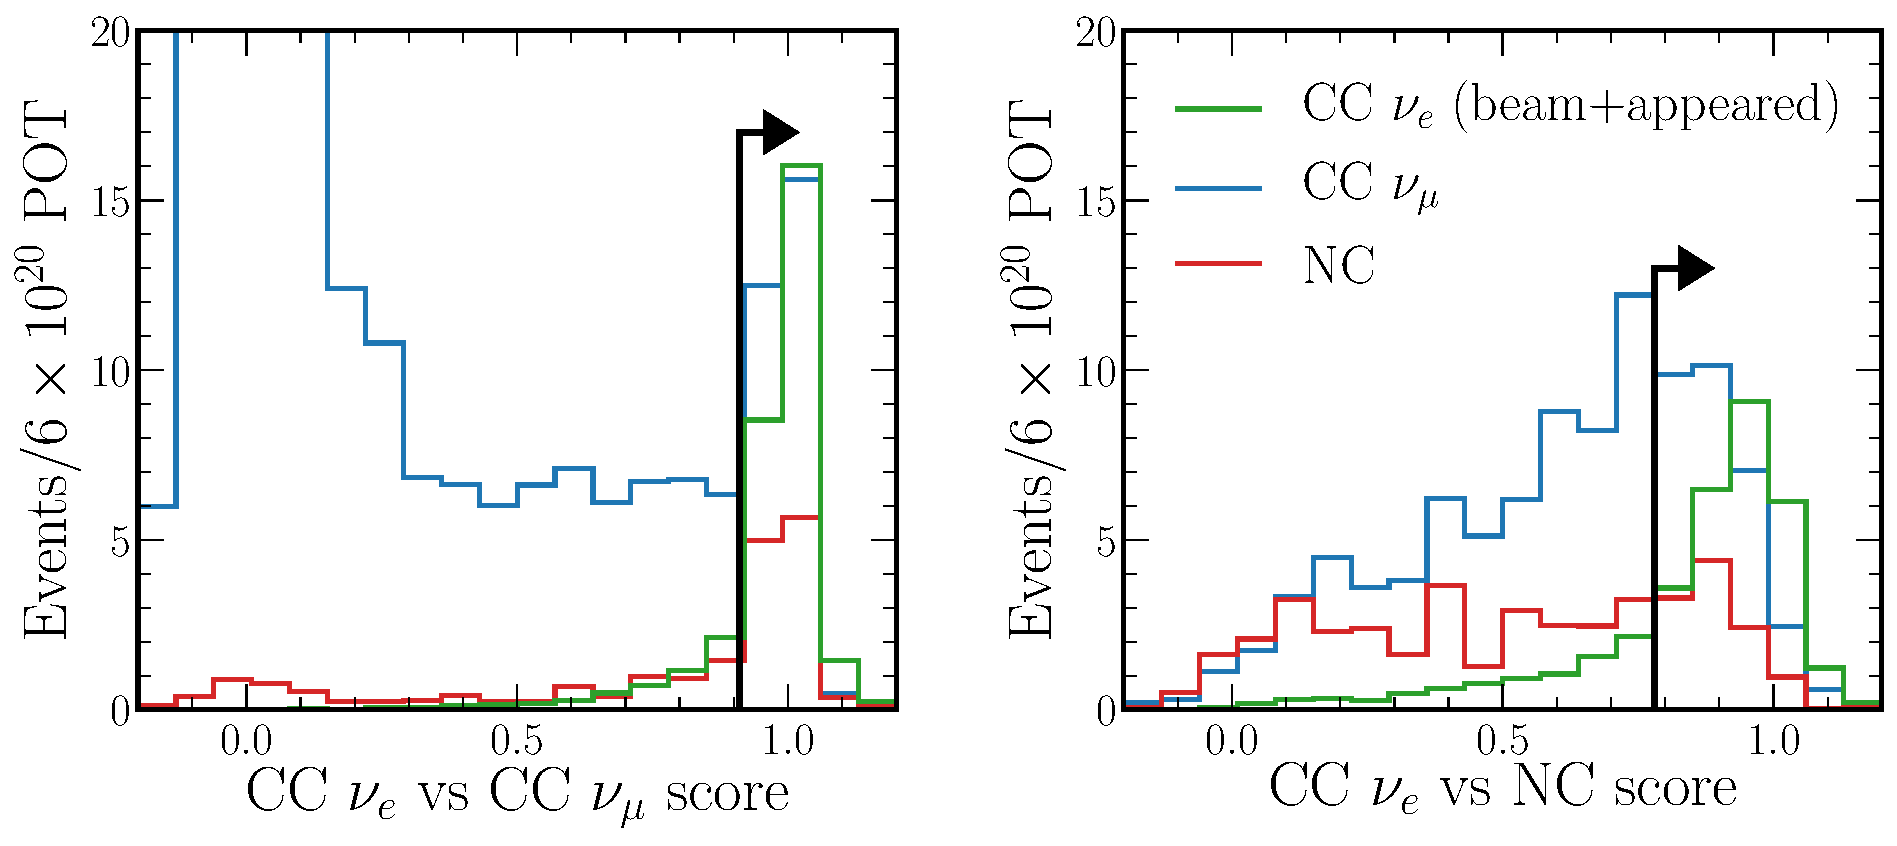
\includegraphics[width=\textwidth]{diagrams/7-results/final_old_pid_outputs.pdf}
    \caption[Distributions of standard event selection neural network output scores]
    {Distributions of CC $\nu_{e}$ vs CC $\nu_{\mu}$ (left) and CC $\nu_{e}$ vs NC (right) output
        scores from the two standard event selection neural networks for the different event
        categories. A score close to one signifies a CC $\nu_{e}$ like event in both cases. Each
        plot shows events which have passed both the preselection and the optimised cut from the
        other network. This is done to better show the events which the network in question
        rejects. Selected CC $\nu_{e}$ events are shown by the arrows. The y-axis for the CC
        $\nu_{e}$ vs CC $\nu_{\mu}$ distributions has been truncated so that the CC $\nu_{\mu}$
        component is not fully visible to better show the distribution of signal CC $\nu_{e}$
        events. Due to the long reconstruction time required, a smaller evaluation sample is used
        here.}
    \label{fig:final_old_pid_outputs}
\end{figure}

\subsubsection*{CC $\nu_{\mu}$ selection} %%%%%%%%%%%%%%%%%%%%%%%%%%%%%%%%%%%%%%%%%%%%%%%%%%%%%%%%

The distribution of CC $\nu_{\mu}$ scores for the different event categories are shown in
\FigureRef{fig:final_beam_numu_outputs}. Excellent separation between appeared CC $\nu_{\mu}$
signal and both CC $\nu_{e}$ components and NC background is achieved. For high CC $\nu_{\mu}$
scores (close to one) the difference between signal and background event counts is approximately
three orders of magnitude.

\begin{figure} % BEAM OUTPUTS NUMU DIAGRAM %
    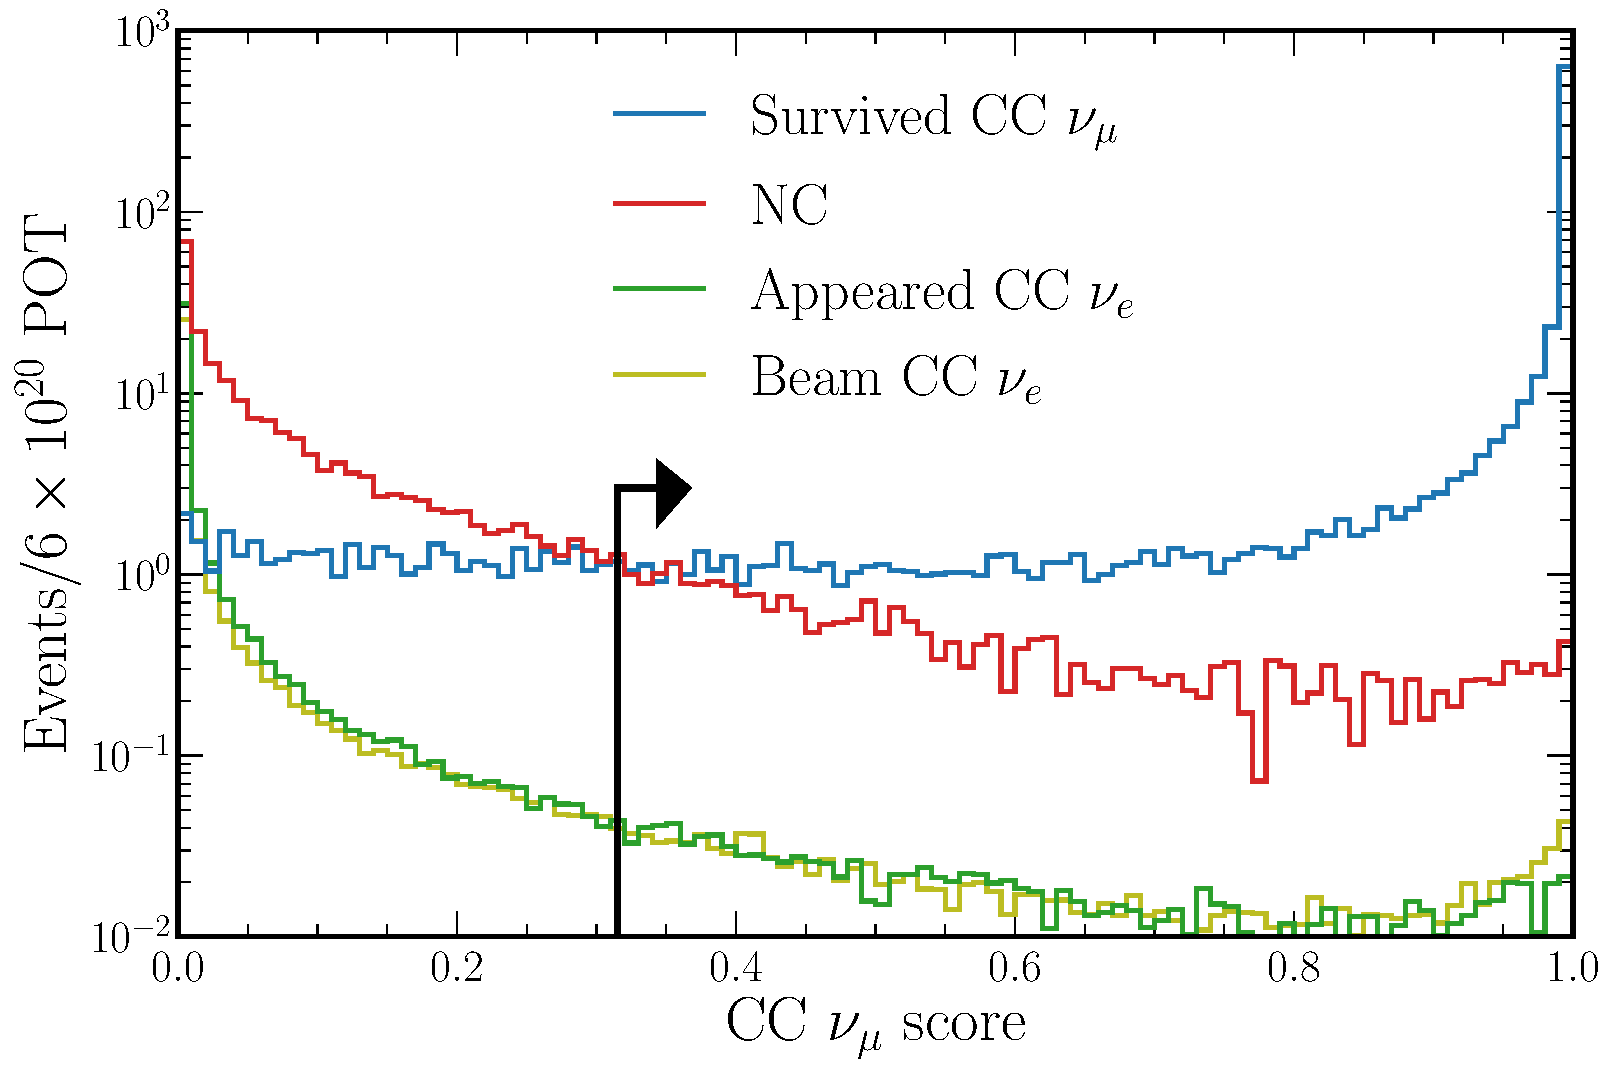
\includegraphics[width=0.7\textwidth]{diagrams/7-results/final_beam_numu_outputs.pdf}
    \caption[Distribution of CC $\nu_{\mu}$ scores from the trained beam classification network]
    {Distribution of \emph{combined category} CC $\nu_{\mu}$ scores from the trained beam
        classification network for the different event categories. A score close to one signifies
        a CC $\nu_{\mu}$ like event.}
    \label{fig:final_beam_numu_outputs}
\end{figure}

The efficiency, purity, and their product (the FOM) for CC $\nu_{\mu}$ events as a function of
selecting events above a particular CC $\nu_{\mu}$ score are shown in
\FigureRef{fig:final_numu_eff_curves}. $\text{Efficiency}\times\text{purity}$ is optimised by
selecting events with a CC $\nu_{\mu}$ score above $0.315$, achieving a value of $0.365$. The
corresponding number and efficiency of selected events for each event category, as well as the
signal purity, are shown in \TableRef{tab:numu_selection}. 

The signal efficiency of 38\% compares well to the 31\% and 36\% achieved by the \nova and T2K CC
$\nu_{\mu}$ selections, respectively~\cite{acero2019, abe2015}. This is also the case for the
signal purity of 96\% compared to the 98.6\% and 94\% purities of the \nova and T2K selections.
Although the final signal efficiency is low, this is desirable to ensure events are fully
contained for energy estimation. When considering just those CC $\nu_{\mu}$ events for which the
primary charged muon is truthfully contained, an 87\% selection efficiency is achieved.

\begin{figure} % FINAL NUMU EFF CURVES DIAGRAM %
    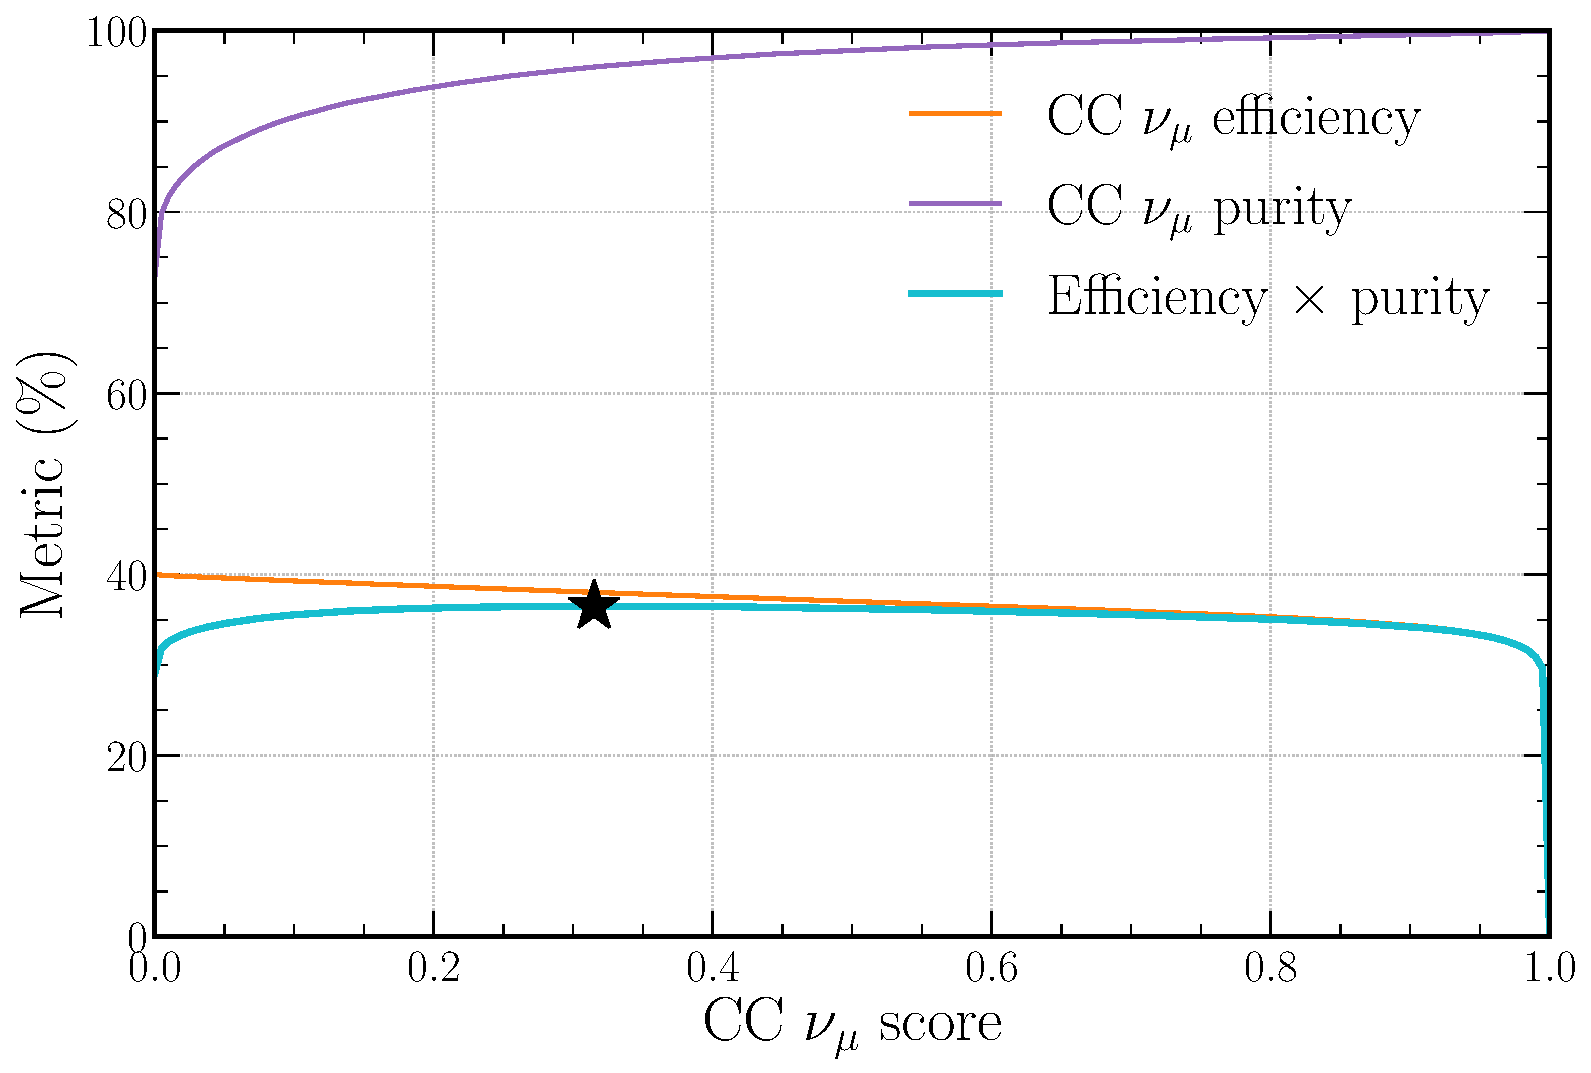
\includegraphics[width=0.7\textwidth]{diagrams/7-results/final_numu_eff_curves.pdf}
    \caption[CC $\nu_{\mu}$ efficiency, purity, and $\text{efficiency}\times\text{purity}$ curves]
    {CC $\nu_{\mu}$ efficiency, purity, and $\text{efficiency}\times\text{purity}$ curves for
        different values of CC $\nu_{\mu}$ score selection.}
    \label{fig:final_numu_eff_curves}
\end{figure}

\begin{table}
    \begin{tabular}{lrrrrr}
                 & CC $\nu_{\mu}$ sig & App CC $\nu_{e}$ bkg & Beam CC $\nu_{e}$ bkg & NC bkg &
                 Sig Purity     \\
        \midrule
        Cuts Num & 818.0              & 40.8                 & 33.0                  & 231.0 &
        $72.9\pm0.5\%$ \\
        FOM Num  & 777.9              & 1.32                 & 1.37                  & 29.3 &
        $96.1\pm0.6\%$ \\
        \midrule
        FOM Eff  & $38.0\pm0.2\%$     & $3.0\pm0.1\%$        & $4.0\pm0.1\%$         &
        $8.4\pm0.2\%$ & -              \\
    \end{tabular}
    \caption[Table showing CC $\nu_{\mu}$ selected event numbers, efficiencies and signal purity]
    {Table showing CC $\nu_{\mu}$ selected event numbers and corresponding efficiencies for the
        various event categories as well as the associated signal purity. Shown are the numbers
        for both the post preselection, \emph{cosmic score} cut, and \emph{escapes score} cut
        numbers (Cuts) in addition to the numbers after the $\text{efficiency}\times\text{purity}$
        (FOM) optimised selection for which the efficiency is shown.}
    \label{tab:numu_selection}
\end{table}

The $\text{efficiency}\times\text{purity}$ optimised CC $\nu_{\mu}$ selection efficiency as a
function of energy for the different event categories is shown in
\FigureRef{fig:final_numu_hists}. Survived CC $\nu_{\mu}$ selection efficiency peaks at just below
\unit{2}{\GeV} before slowly declining, this is explained by higher energy events being less
likely to have their primary charged muon fully contained within the detector. Of interest is the
expected dip in the otherwise very high ($>90\%$) CC $\nu_{\mu}$ purity at approximately
\unit{1.5}{\GeV}, corresponding to the oscillation maximum (shown in
\FigureRef{fig:osc_cp_probs}). As in the CC $\nu_{e}$ selection case, the NC efficiency is seen to
rise with energy, again likely due to misidentification of energetic protons and pions.

\begin{figure} % FINAL NUMU HISTS DIAGRAM %
    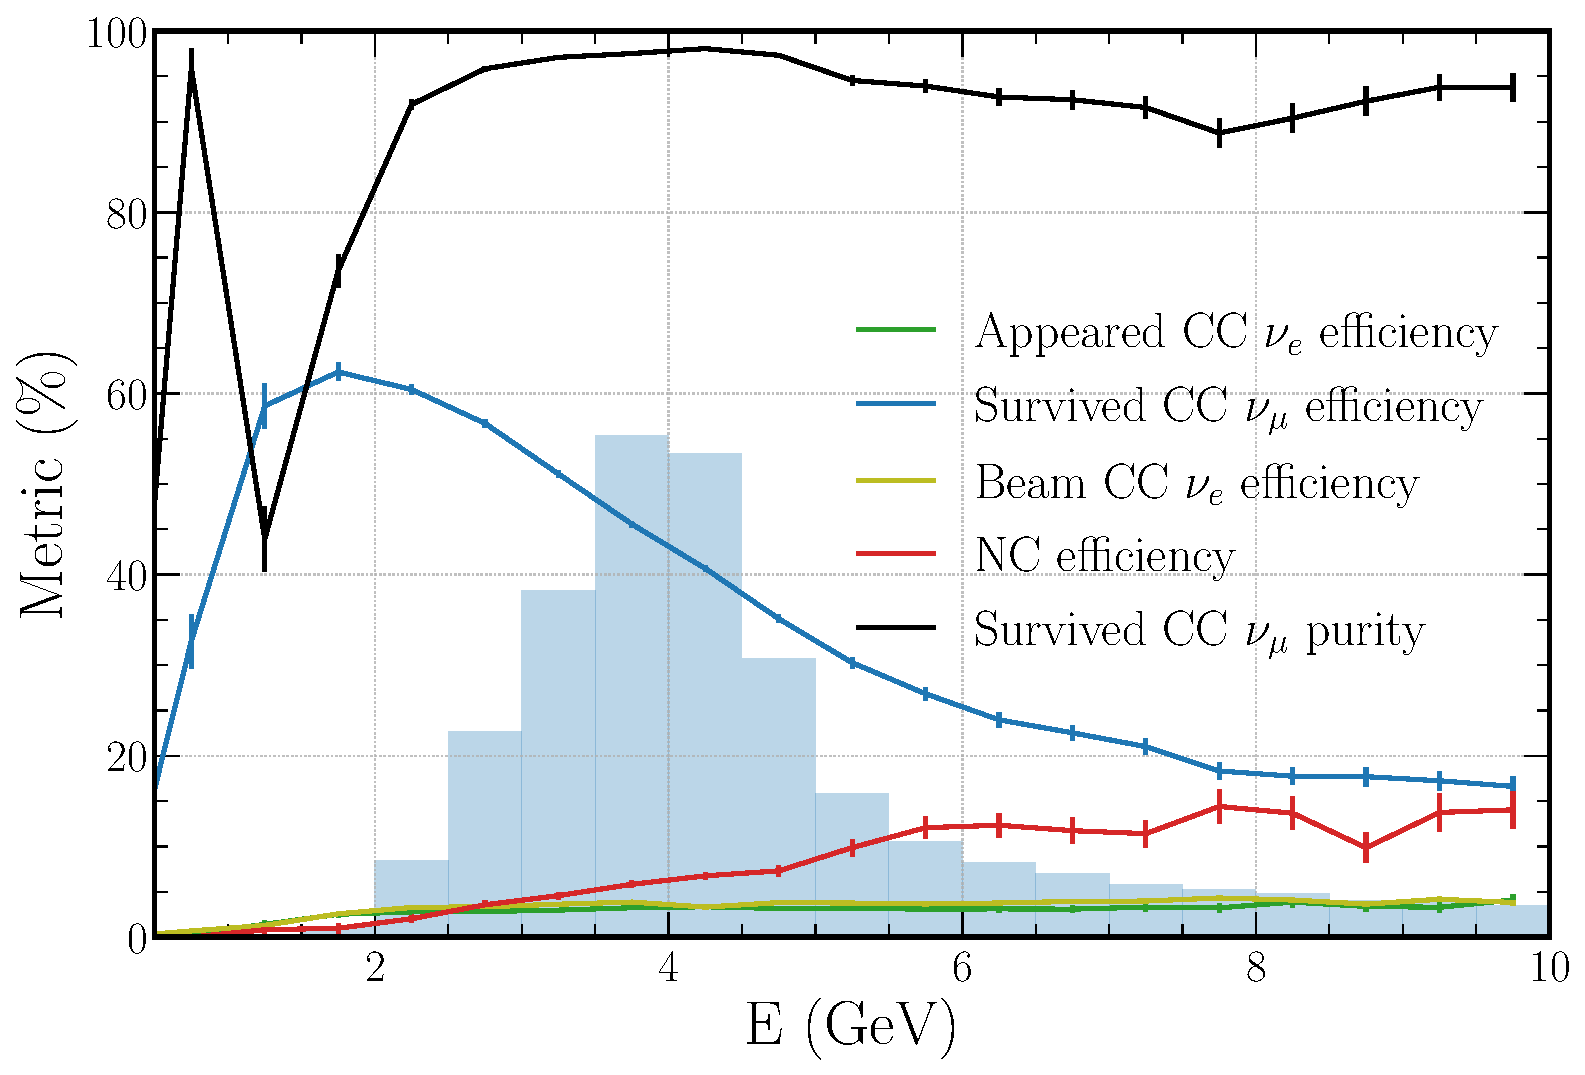
\includegraphics[width=0.7\textwidth]{diagrams/7-results/final_numu_hists.pdf}
    \caption[Efficiency of the CC $\nu_{\mu}$ selection as a function of energy]
    {Efficiency of the CC $\nu_{\mu}$ selection for the different event categories as well as
        survived CC $\nu_{\mu}$ purity as a function of neutrino energy. All CC categories are
        shown in terms of neutrino energy, while NC events are shown in terms of the hadronic
        component energy. For reference, the true survived CC $\nu_{\mu}$ neutrino energy
        distribution is shown in the blue.}
    \label{fig:final_numu_hists}
\end{figure}

\subsubsection*{Interaction type classification} %%%%%%%%%%%%%%%%%%%%%%%%%%%%%%%%%%%%%%%%%%%%%%%%%

Using the \emph{CC category} output of the trained beam classification network, the CC interaction
type (used for energy estimation in \SectionRef{sec:results_eval_energy}) for both CC $\nu_{e}$
and CC $\nu_{\mu}$ selected events can be determined. As in the \emph{combined category} output
case, the highest-scoring neuron can be used for classification, resulting in the matrix shown in
\FigureRef{fig:final_cc_cat_confusion}. Note that only events which are selected by either the CC
$\nu_{e}$ or CC $\nu_{\mu}$ selection are shown.

\begin{figure} % FINAL CC CAT CONFUSION DIAGRAM %
    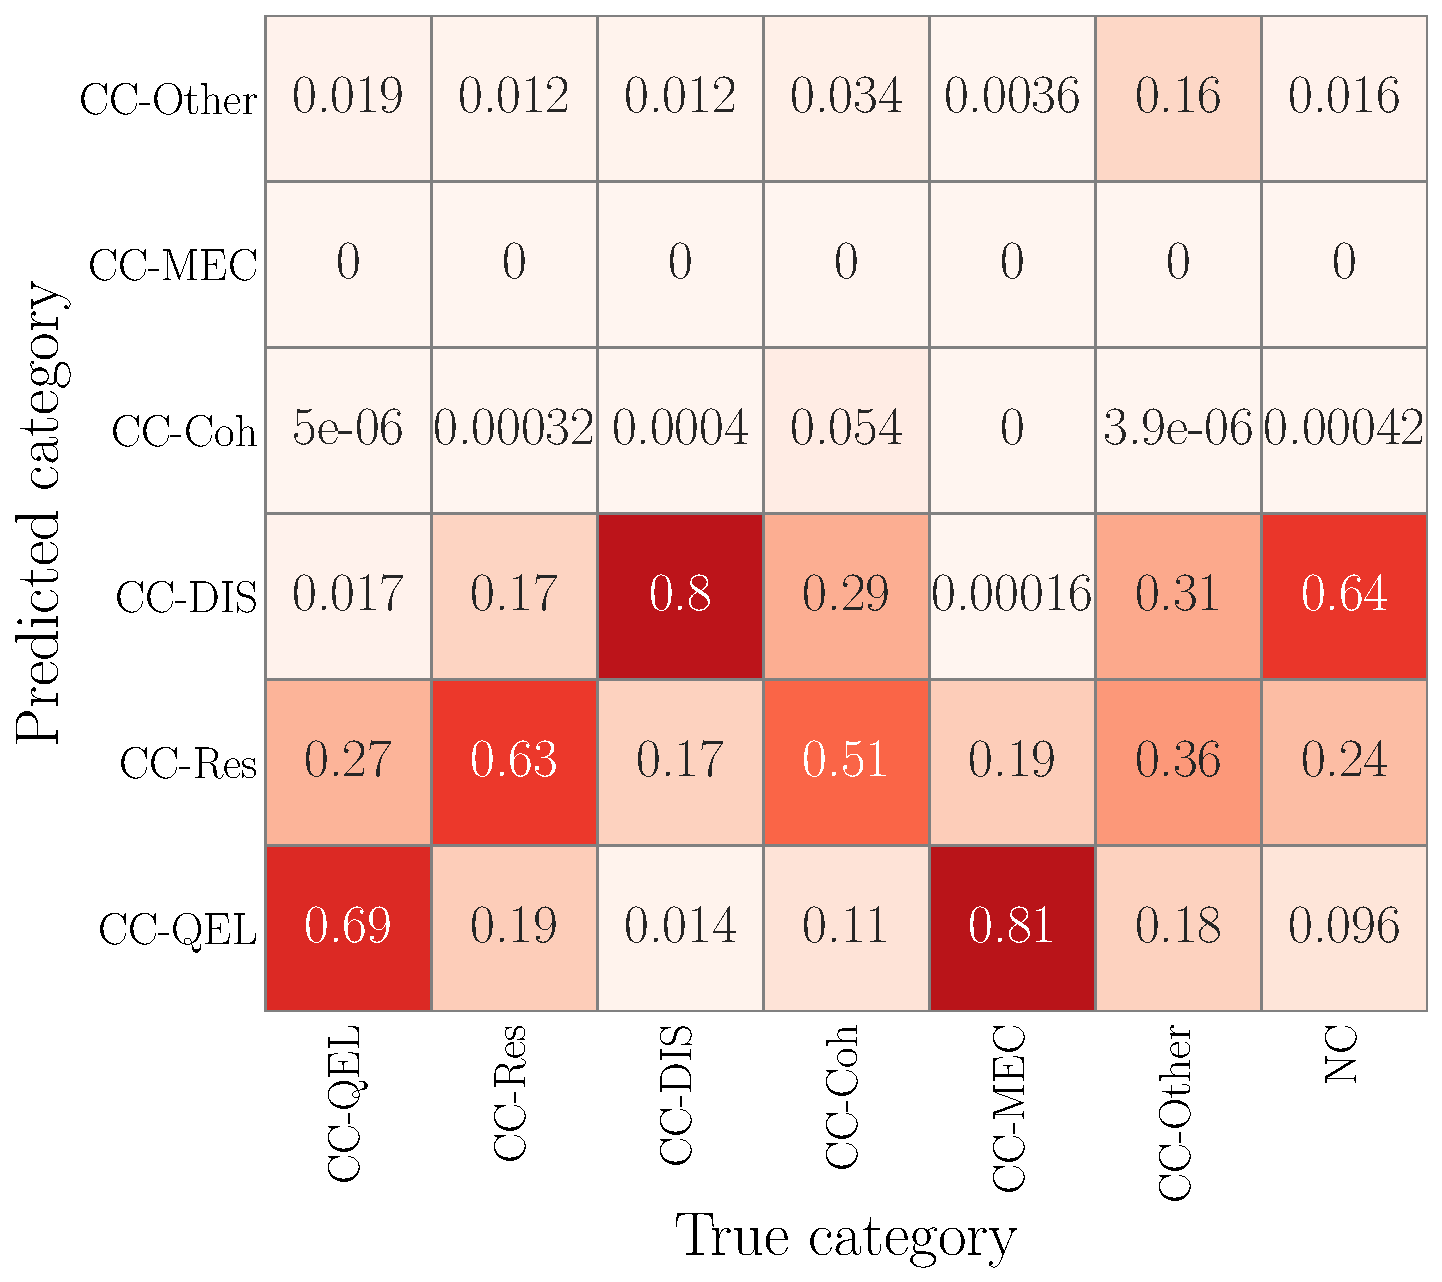
\includegraphics[width=0.8\textwidth]{diagrams/7-results/final_cc_cat_confusion.pdf}
    \caption[Classification matrix for the CC category output of the beam classification network]
    {Classification matrix for the \emph{CC category} output of the trained beam classification
        network. Shown are events that have either been selected by the CC $\nu_{e}$ or CC
        $\nu_{\mu}$ selection. Events are simply classified using the categorical score for which
        they have the highest value. The numbers shown are the fraction of true category events
        classified into each of the six possible categories.}
    \label{fig:final_cc_cat_confusion}
\end{figure}

Reasonable classification accuracy greater than 60\% is achieved across the three dominant
interaction types, CC-QEL, CC-Res, and CC-DIS. The less common CC-Coh and CC-MEC types are found
to be commonly misidentified as CC-Res and CC-QEL respectively, likely due to the imbalanced
training dataset and their corresponding topological similarities. Background NC events which pass
either CC $\nu_{e}$ or CC $\nu_{\mu}$ selection (commonly high in energy) are found to be
typically classified as CC-DIS; this is expected as they commonly contain multiple energetic
particles in the final state.

For completeness, the \emph{NC category} classification matrix is shown in
\FigureRef{fig:final_nc_cat_confusion} for events that are neither classified as CC $\nu_{e}$ or
CC $\nu_{\mu}$. As in the CC case, the dominant interaction types NC-Res and NC-DIS are classified
well, with NC-Coh events typically being classified as NC-Res. Of the CC events that are not
selected, the vast majority are classified as NC-DIS events. Similarly to before, this is likely
due to multiple energetic particles in the final state, for which the beam classification network
determined no clear charged lepton.

\begin{figure} % FINAL NC CAT CONFUSION DIAGRAM %
    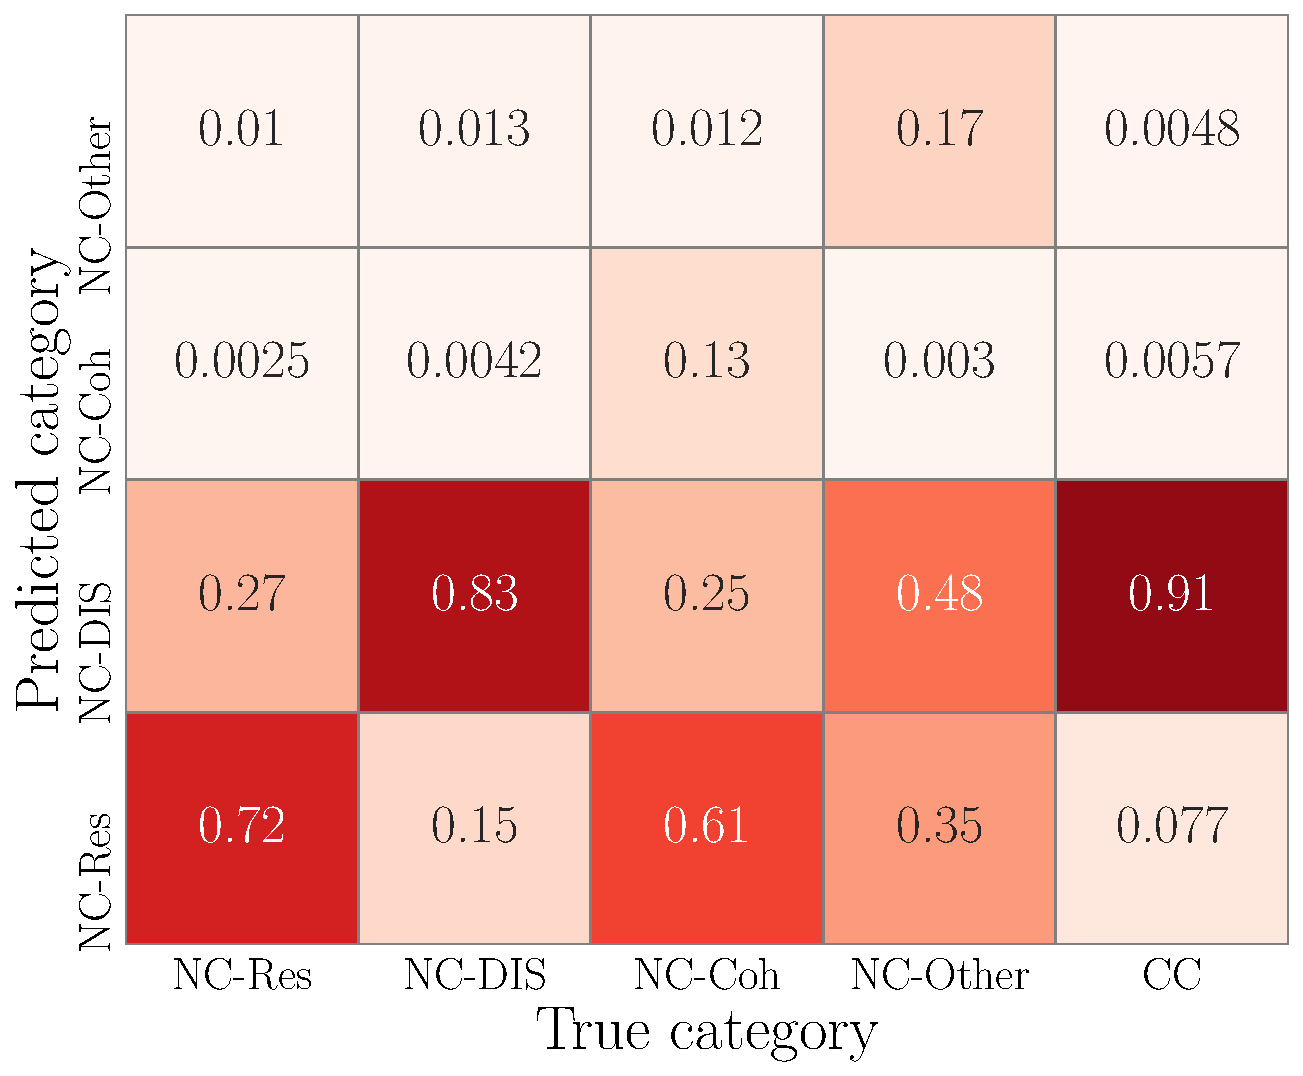
\includegraphics[width=0.7\textwidth]{diagrams/7-results/final_nc_cat_confusion.pdf}
    \caption[Classification matrix for the NC category output of the beam classification network]
    {Classification matrix for the \emph{NC category} output of the trained beam classification
        network. Events are simply classified using the categorical score for which they have the
        highest value. The numbers shown are the fraction of true category events classified into
        each of the four possible categories.}
    \label{fig:final_nc_cat_confusion}
\end{figure}

\subsection{Energy and vertex estimation} %%%%%%%%%%%%%%%%%%%%%%%%%%%%%%%%%%%%%%%%%%%%%%%%%%%%%%%%
\label{sec:results_eval_energy} %%%%%%%%%%%%%%%%%%%%%%%%%%%%%%%%%%%%%%%%%%%%%%%%%%%%%%%%%%%%%%%%%%

By using the CC interaction type classification just presented, the differences between CC
interaction types can be exploited to improve neutrino energy, charged lepton energy, and
interaction vertex position and time estimation. For events classified as either CC $\nu_{e}$ or
CC $\nu_{\mu}$ with an associated \emph{CC category} interaction type, the corresponding bespoke
trained network outlined in \SectionRef{sec:cnn_specific_energy} is used for estimation.

Only three networks for each neutrino type are trained, one for each of the dominant interaction
types CC-QEL (and CC-MEC), CC-Res, and CC-DIS. For events not classified by the \emph{CC category}
output as one of these categories, such as CC-Coh or CC-Other, the CC-Res network is used as it is
the most topologically similar interaction type.

\subsubsection*{Energy estimation} %%%%%%%%%%%%%%%%%%%%%%%%%%%%%%%%%%%%%%%%%%%%%%%%%%%%%%%%%%%%%%%

The distributions of CNN estimated (\emph{neutrino energy} output) and true $\nu_{e}$ and
$\nu_{\mu}$ neutrino energies for true CC $\nu_{e}$ and CC $\nu_{\mu}$ events respectively that
are also selected by their corresponding CC selection are shown in
\FigureRef{fig:final_energy_dists}. The CNN estimated distributions match the truth well across
the full range of neutrino energies expected within \chipsfive, except in the peak regions where
the truth distribution shape is not fully captured.

\begin{figure} % FINAL ENERGY DISTS DIAGRAM %
    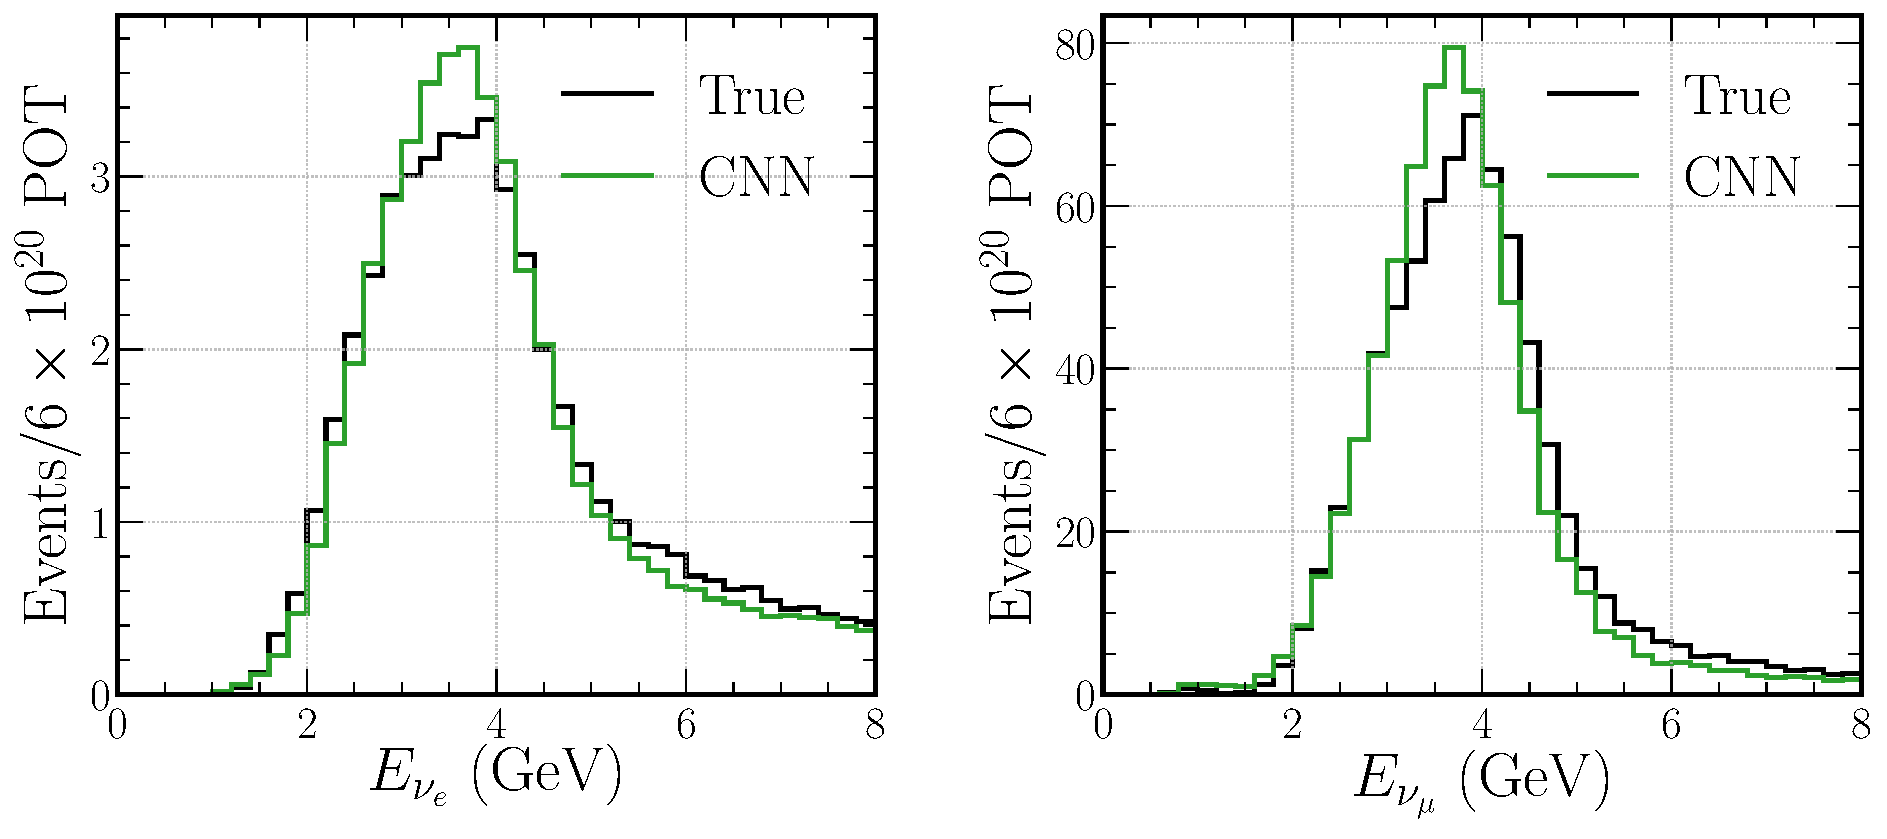
\includegraphics[width=\textwidth]{diagrams/7-results/final_energy_dists.pdf}
    \caption[Distributions of true and CNN estimated neutrino energy]
    {Distributions of true and CNN estimated neutrino energy for CC $\nu_{e}$ (left) and CC
        $\nu_{\mu}$ (right) beam events. Only true CC $\nu_{e}$ and CC $\nu_{\mu}$ events that are
        also selected by the CC $\nu_{e}$ and CC $\nu_{\mu}$ selections respectively are shown.}
    \label{fig:final_energy_dists}
\end{figure}

As the training samples contain a spectrum of events typical of the beam, it is important to check
that the CNN neutrino energy estimation is not simply predicting an energy close to the expected
peak beam energy. The probability of a CNN estimated neutrino energy given a true neutrino energy
is shown in \FigureRef{fig:final_energy_2d} for both CC $\nu_{e}$ and CC $\nu_{\mu}$ events. CNN
estimated energy is found to be roughly equivalent to true energy across the full range of
expected \chipsfive beam energies, proving the desired response.

\begin{figure} % FINAL 2D ENERGY DIAGRAM %
    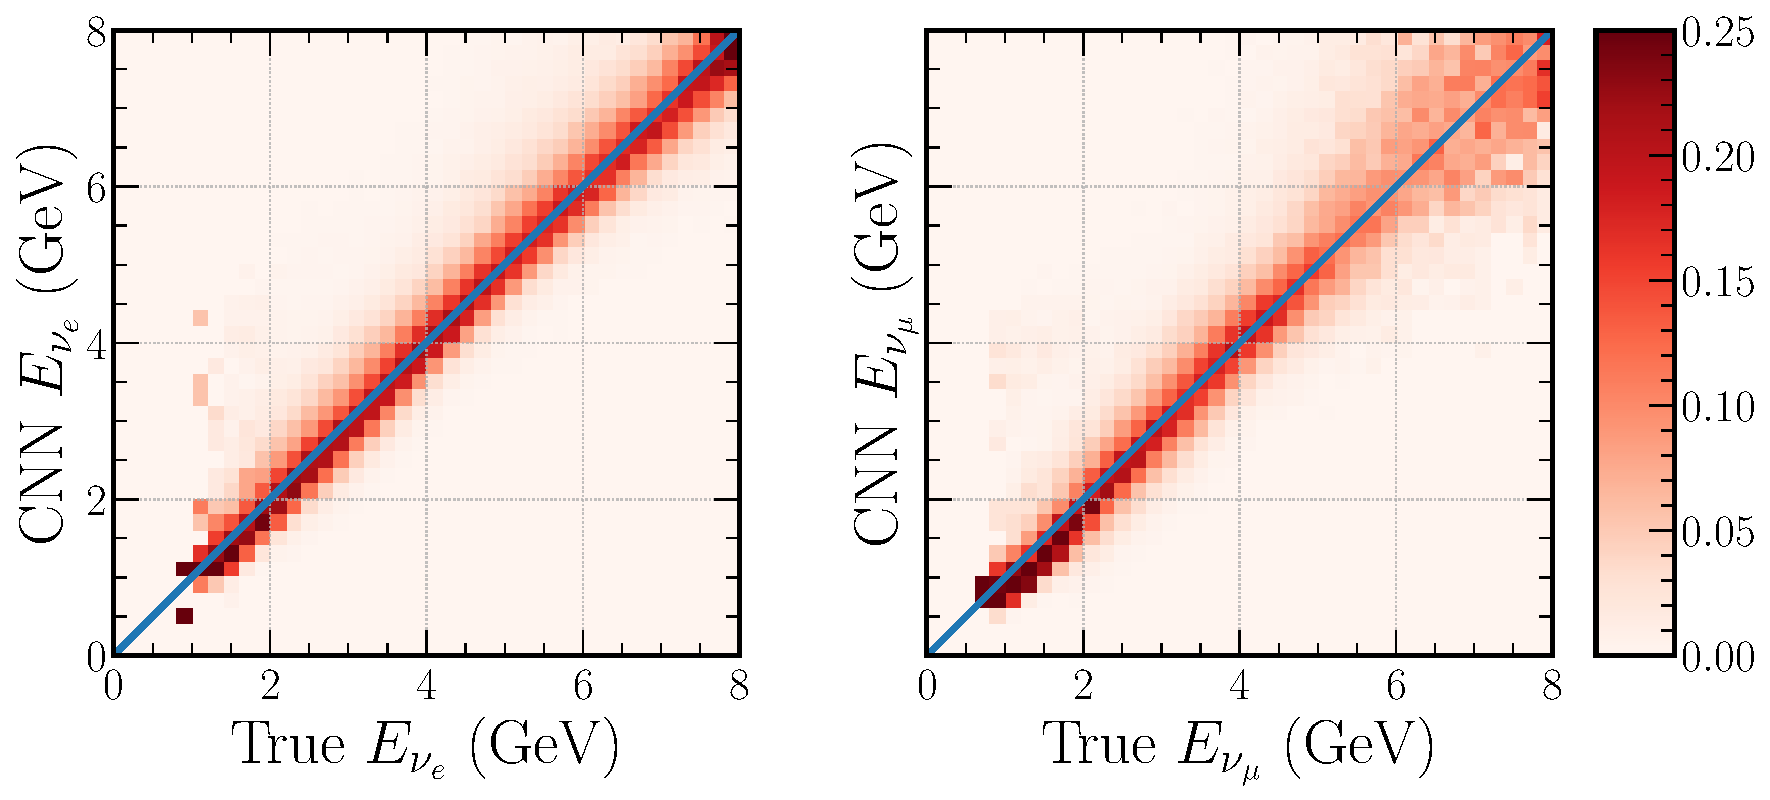
\includegraphics[width=\textwidth]{diagrams/7-results/final_energy_2d.pdf}
    \caption[Probability of CNN estimated neutrino energy given a true neutrino energy]
    {Probability of CNN estimated neutrino energy given a true neutrino energy for CC $\nu_{e}$
        (left) and CC $\nu_{\mu}$ (right) beam events, with their equality shown in blue. Only
        true CC $\nu_{e}$ and CC $\nu_{\mu}$ events that are also selected by the CC $\nu_{e}$ and
        CC $\nu_{\mu}$ selections respectively are shown.}
    \label{fig:final_energy_2d}
\end{figure}

To fully understand CNN energy estimation performance, histograms of ratios of differences between
CNN estimated (reco) and true neutrino energy to true neutrino energy for both CC $\nu_{e}$ and CC
$\nu_{\mu}$ beam events are shown in \FigureRef{fig:final_energy_frac}. Distributions are shown
for both \emph{all} selected events and just the true \emph{signal} component within the
corresponding beam selection. Similar distributions splitting the \emph{signal} component by
interaction type are shown in \FigureRef{fig:final_energy_frac_split}. Furthermore, a summary of
the neutrino energy resolutions achieved for both CC $\nu_{e}$ and CC $\nu_{\mu}$ events is shown
in \TableRef{tab:energy_resolutions}.

\begin{figure} % FINAL ENERGY FRAC DIAGRAM %
    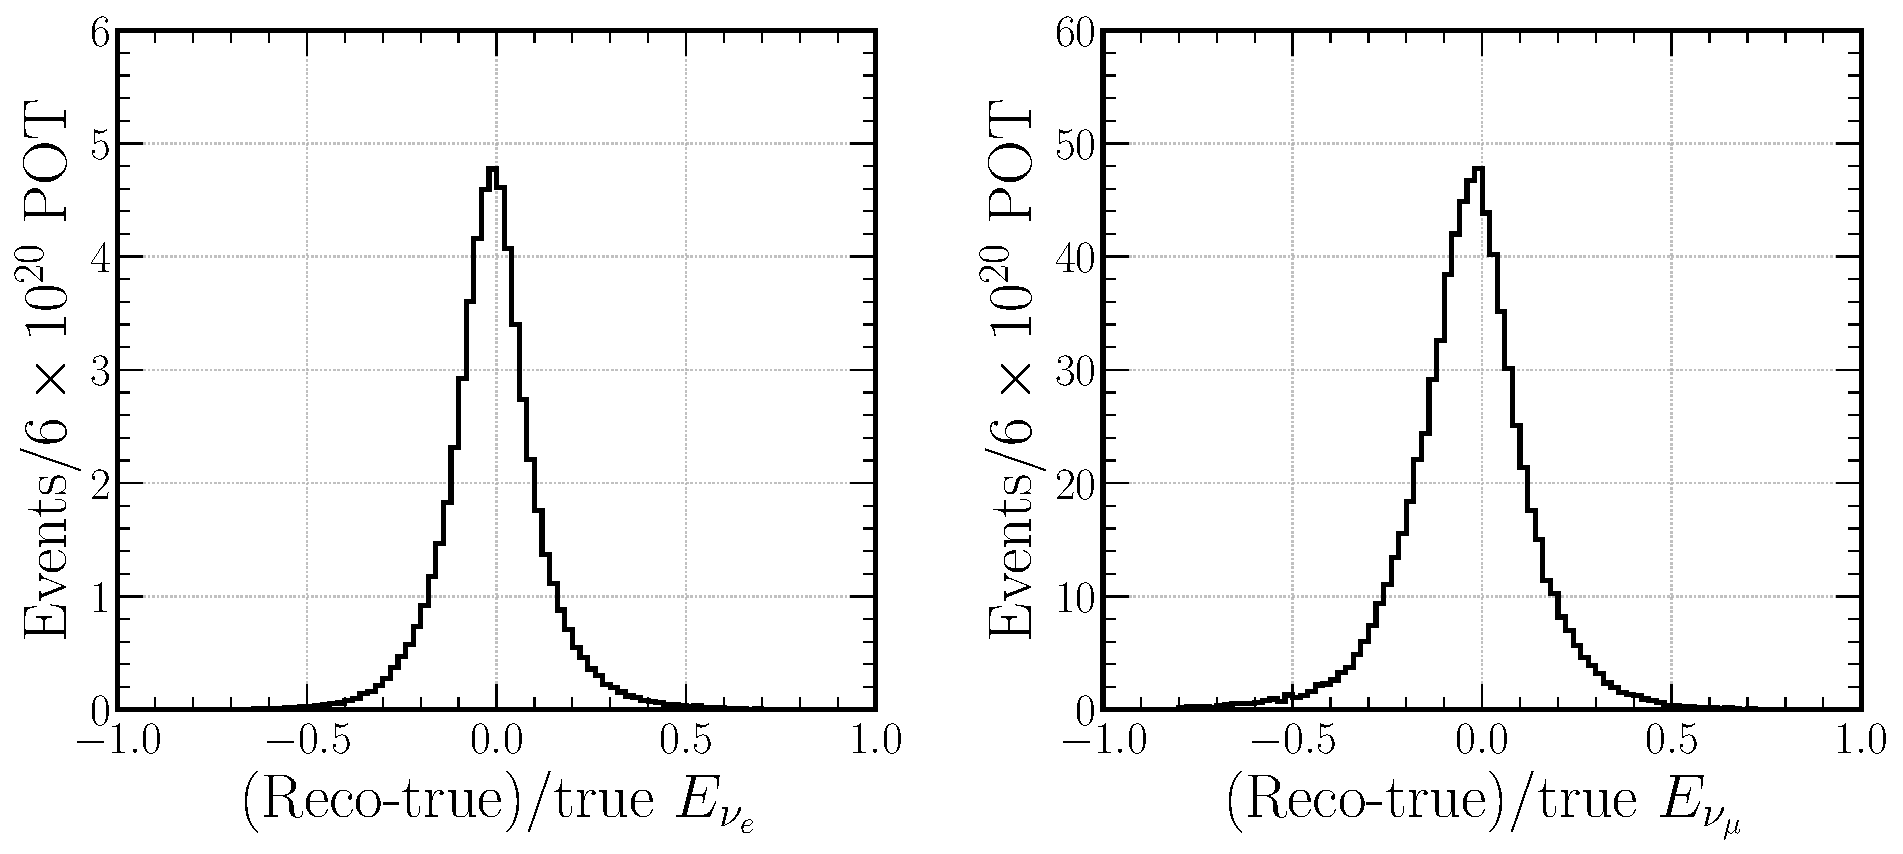
\includegraphics[width=\textwidth]{diagrams/7-results/final_energy_frac.pdf}
    \caption[Distributions of (reco-true)/true neutrino energies]
    {Distributions of (reco-true)/true neutrino energies for both CC $\nu_{e}$ (left) and CC
        $\nu_{\mu}$ (right) beam events. Distributions for both \emph{all} respectively selected
        events and just the \emph{signal} component of each selection are shown.}
    \label{fig:final_energy_frac}
\end{figure}

\begin{figure} % FINAL ENERGY FRAC SPLIT DIAGRAM %
    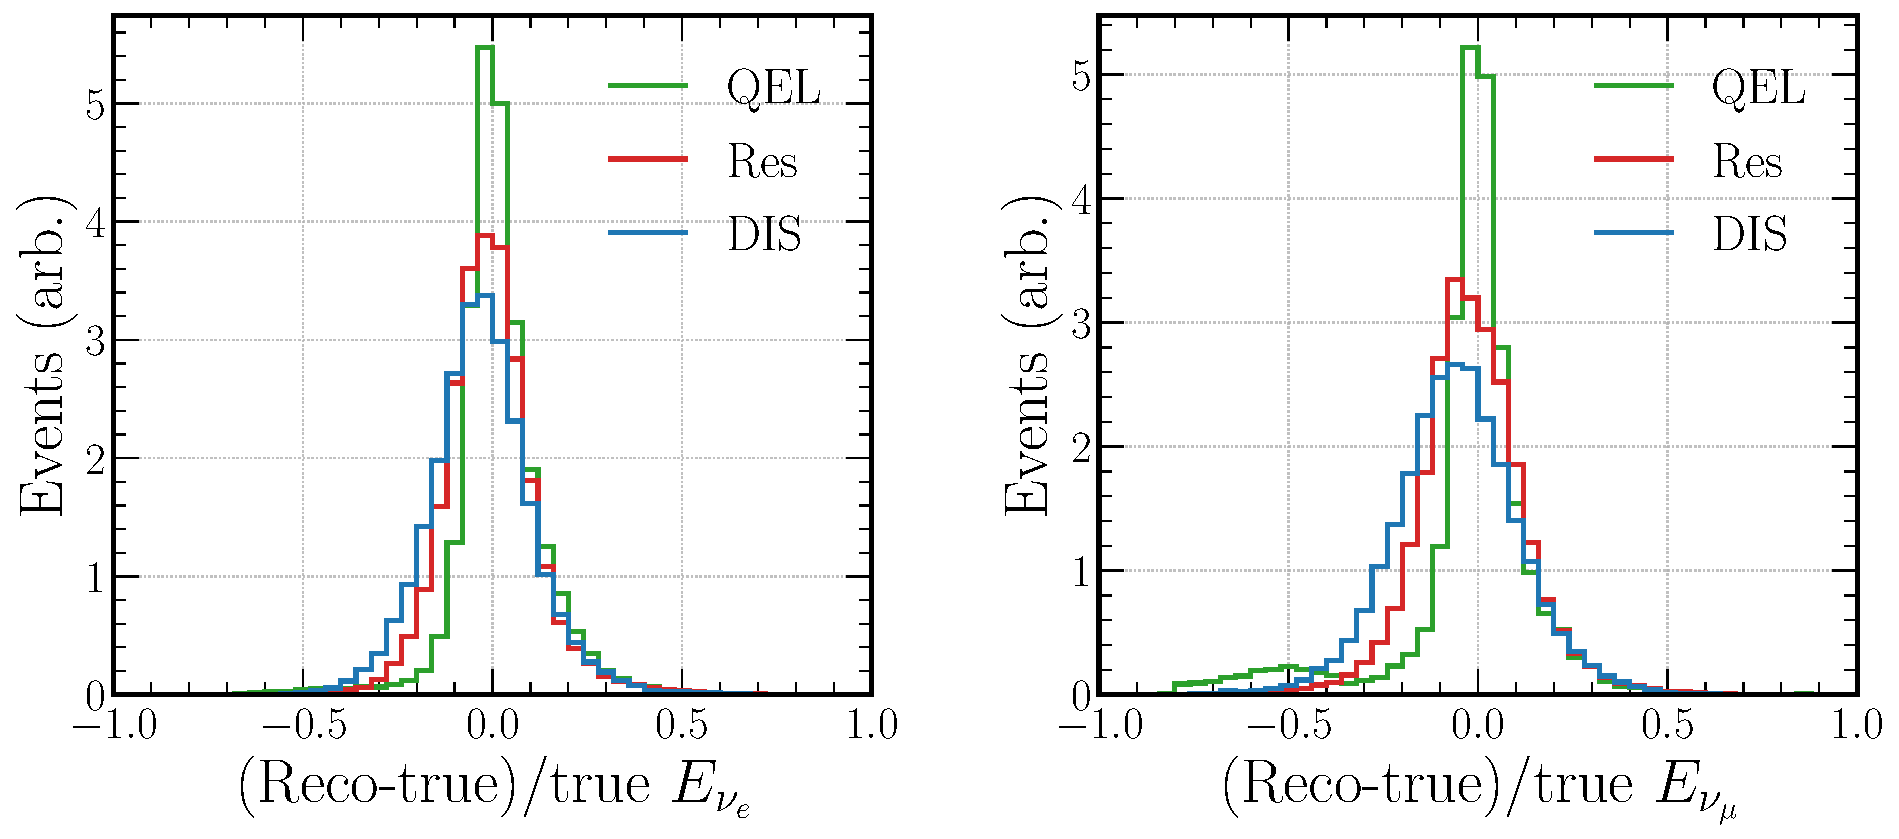
\includegraphics[width=\textwidth]{diagrams/7-results/final_energy_frac_split.pdf}
    \caption[Distributions of (reco-true)/true neutrino energies by interaction type]
    {Distributions of (reco-true)/true neutrino energies for both CC $\nu_{e}$ (left) and CC
        $\nu_{\mu}$ (right) signal beam events by interaction types. The relative number of events
        between interaction types has been scaled for clearer comparison.}
    \label{fig:final_energy_frac_split}
\end{figure}

\begin{table}
    \begin{tabular}{lrrrrr}
        Event type     & All    & Signal & Signal-QEL & Signal-Res & Signal-DIS \\
        \midrule
        CC $\nu_{e}$   & 12.9\% & 10.3\% & 7.1\%      & 10.3\%     & 13.6\%     \\
        CC $\nu_{\mu}$ & 12.9\% & 12.6\% & 6.2\%      & 11.7\%     & 14.9\%     \\
    \end{tabular}
    \caption[Summary of CC $\nu_{e}$ and CC $\nu_{\mu}$ neutrino energy resolutions]
    {Summary of CC $\nu_{e}$ and CC $\nu_{\mu}$ neutrino energy resolutions. Shown for each sample
        are the resolutions for \emph{all} selected events, the true \emph{signal} selected events
        and the three dominant \emph{signal} interaction type components, QEL, Res, and DIS. The
        resolutions are calculated from the standard deviations of gaussian fits made to the
        distributions shown in \FigureRef{fig:final_energy_frac} and
        \FigureRef{fig:final_energy_frac_split}.}
    \label{tab:energy_resolutions}
\end{table}

The tail of negative values for the \emph{all} selected CC $\nu_{e}$ distribution in
\FigureRef{fig:final_energy_frac} indicates that wrongly classified CC $\nu_{e}$ events, mainly NC
in nature, are typically estimated with a neutrino energy lower than the actual value. This is
expected given the missing energy of the final state neutrino. Additionally, the interaction type
resolutions follow the expected pattern, with the simple to reconstruct single charged lepton QEL
interactions achieving a stronger resolution than multi-particle DIS events. Furthermore, these
results are similar to the selected signal energy resolutions obtained by \nova of 10.7\% for CC
$\nu_{e}$ events and 9.1\% for CC $\nu_{\mu}$ events~\cite{acero2019}.

By making gaussian fits to the (reco-true)/true signal neutrino energy distributions shown in
\FigureRef{fig:final_energy_frac} in \unit{1}{GeV} wide true neutrino energy bins, the energy
dependence of the energy resolution can be explored. The means and standard deviations of these
fits are shown in \FigureRef{fig:final_energy_nuel} and \FigureRef{fig:final_energy_numu} for CC
$\nu_{e}$ and CC $\nu_{\mu}$ events respectively, split by interaction type.

Reasonably significant bias in the means is observed with respect to the true neutrino energy for
both CC $\nu_{e}$ and CC $\nu_{\mu}$ events. This is particularly true of DIS events, but still
significant for Res and QEL events. As the energy spectrum of events used for training peaks, this
is expected. Any future energy estimation work should consider using a flat energy spectrum for
training, as done in \ReferenceRef{baldi2019}.

The standard deviation is seen to decrease with true neutrino energy for all interaction types,
except for energies above the flux peak. Again, this is most likely due to the spectrum of events
used in the training sample. A contributing factor, however, will be due to the inability of PMTs
to distinguish between numbers of incident photons at higher counts, more likely at higher
energies.

\begin{figure} % FINAL NUEL ENERGY DIAGRAM %
    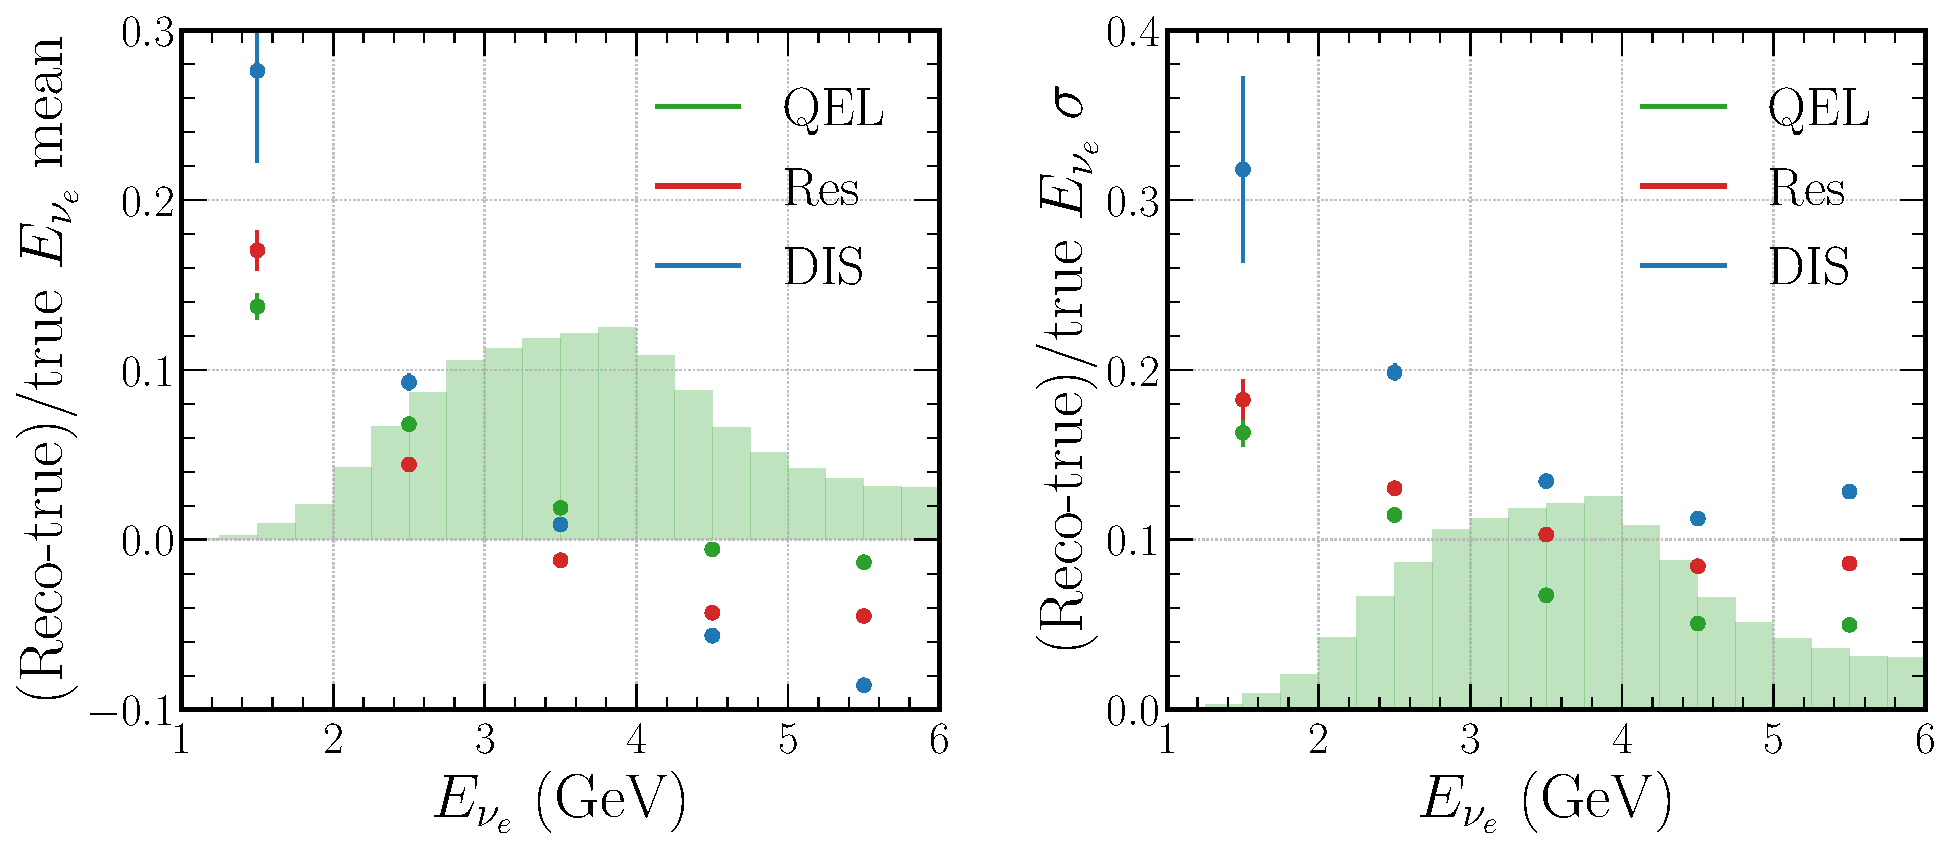
\includegraphics[width=\textwidth]{diagrams/7-results/final_energy_nuel.pdf}
    \caption[Means and standard deviations of fits to $\nu_{e}$ energy distributions]
    {Means (left) and standard deviations (right) of gaussian fits made to distributions of
        (reco-true)/true neutrino energy for CC $\nu_{e}$ events across a range of \unit{1}{GeV}
        wide true neutrino energy bins and split by interaction type. The true distribution of CC
        $\nu_{e}$ events is shown in green.}
    \label{fig:final_energy_nuel}
\end{figure}

\begin{figure} % FINAL NUMU ENERGY DIAGRAM %
    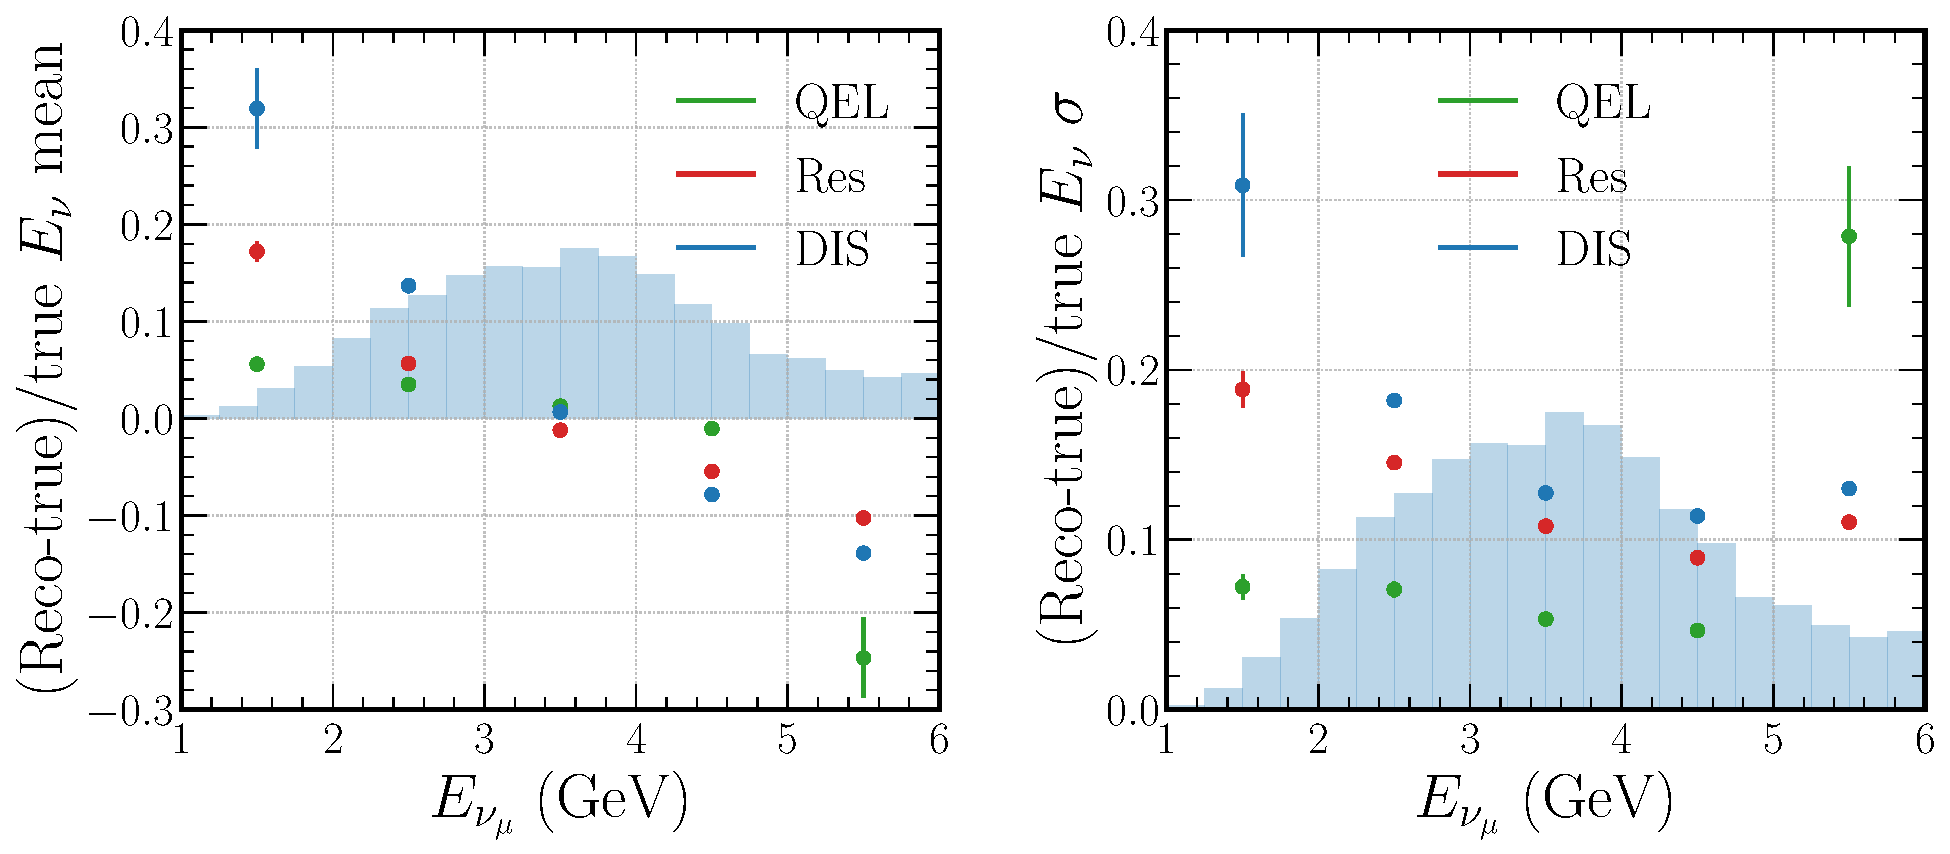
\includegraphics[width=\textwidth]{diagrams/7-results/final_energy_numu.pdf}
    \caption[Means and standard deviations of fits to $\nu_{\mu}$ energy distributions]
    {Means (left) and standard deviations (right) of gaussian fits made to distributions of
        (reco-true)/true neutrino energy for CC $\nu_{\mu}$ events across a range of \unit{1}{GeV}
        wide true neutrino energy bins and split by interaction type. The true distribution of CC
        $\nu_{\mu}$ events is shown in blue.}
    \label{fig:final_energy_numu}
\end{figure}

As in the CC $\nu_{e}$ selection case, the best way to understand the relative performance of the
energy estimation is by comparison with the standard \chips reconstruction presented in
\SectionRef{sec:cnn_old_reco}. Although the standard reconstruction does not attempt to estimate
the neutrino energy, the energy of the primary charged lepton in each CC event is predicted. The
value can be compared to the \emph{charged lepton energy} output of the energy estimation CNNs.
Histograms of ratios of differences between CNN estimated (reco) and true charged lepton energy to
true charged lepton energy for both CC $\nu_{e}$ and CC $\nu_{\mu}$ beam QEL events are shown in
\FigureRef{fig:final_frac_e_comparison}.

A significant improvement is made using the new CNN approach. An energy resolution 32\% and 40\%
the size of the standard reconstruction resolution for CC $\nu_{e}$ and $\nu_{\mu}$ QEL events
respectively is achieved, at 4.5\% and 4.0\%. When compared to the approximately 2.5\% CC QEL
charged lepton energy resolution reached by the Super-Kamiokande fiTQun
algorithm~\cite{jiang2019}, the performance presented here is impressive, particularly given the
significant differences in detector design.

\begin{figure} % FINAL FRAC E COMPARISON DIAGRAM %
    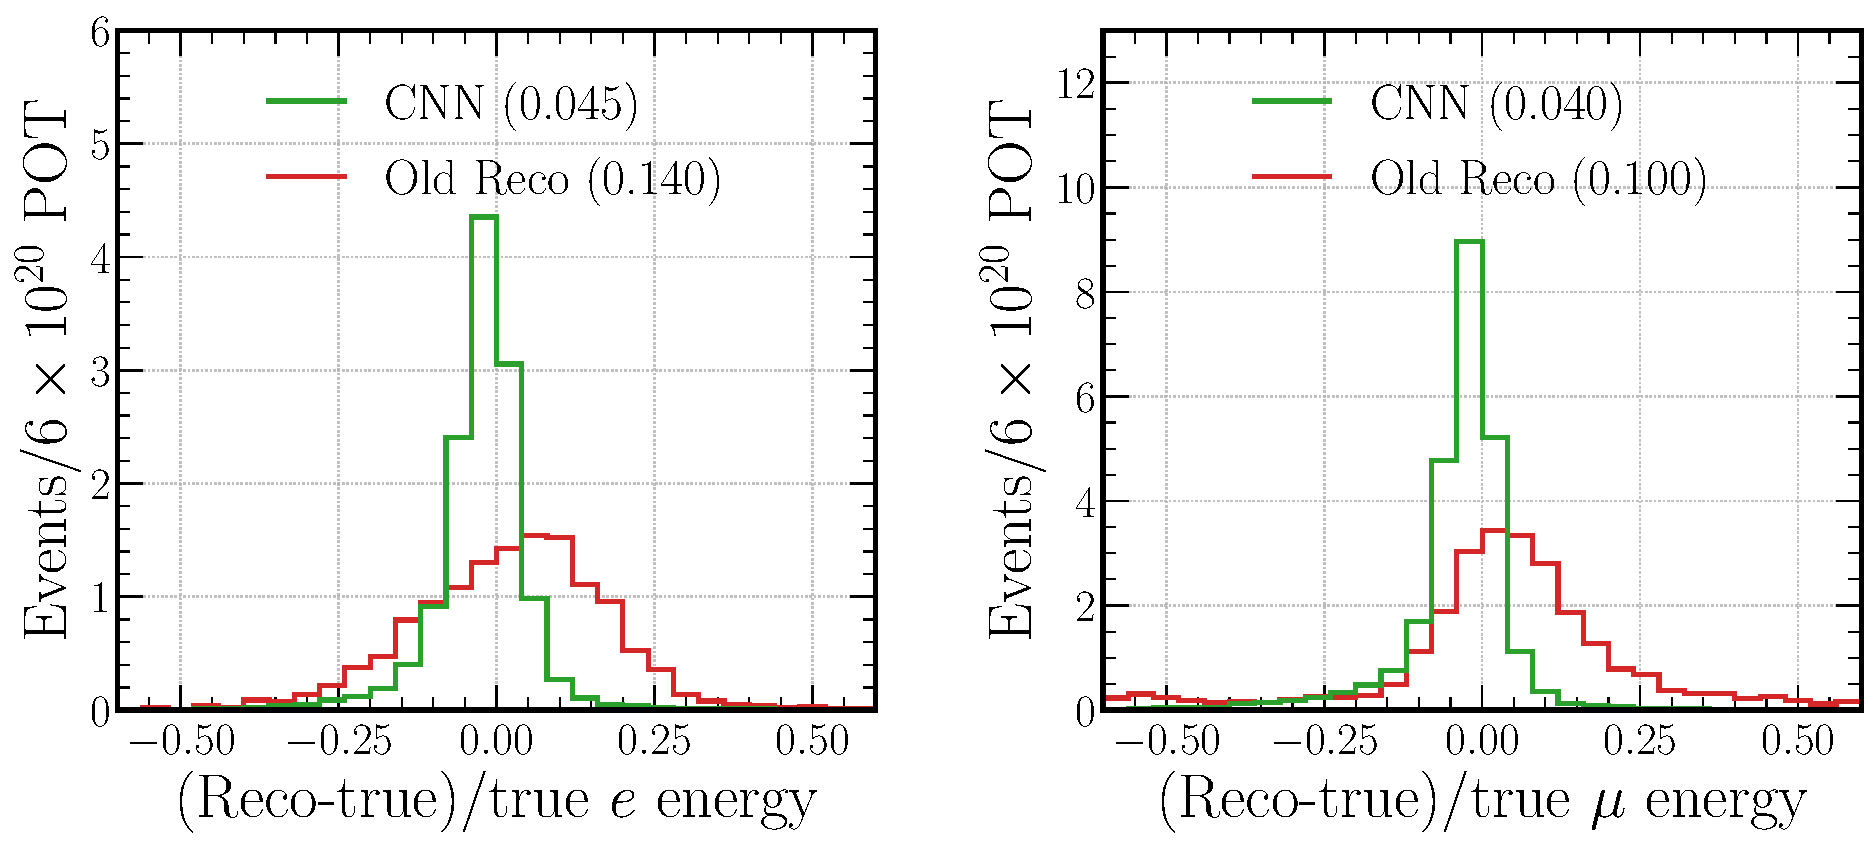
\includegraphics[width=\textwidth]{diagrams/7-results/final_frac_e_comparison.pdf}
    \caption[Distributions of (reco-true)/true primary charged lepton energies for the CNN and
        standard methods] {Distributions of (reco-true)/true primary charged lepton energies for
        both CC $\nu_{e}$ (left) and CC $\nu_{\mu}$ (right) beam events for both the new CNN
        approach and standard (old) methods. Only QEL events are shown for clearer comparison with
        the standard reconstruction methods. The standard deviation of a gaussian fit made to each
        distribution is shown in the corresponding brackets.}
    \label{fig:final_frac_e_comparison}
\end{figure}

\subsubsection*{Interaction vertex estimation} %%%%%%%%%%%%%%%%%%%%%%%%%%%%%%%%%%%%%%%%%%%%%%%%%%%

The \emph{interaction vertex x-position}, \emph{interaction vertex y-position}, \emph{interaction
    vertex z-position}, and \emph{interaction time} outputs from the energy estimation networks
    can also be used. Although not employed in this work, future analyses may require accurate
    fiducial volume cuts or separation of events in time, therefore, strong performance is
    desirable. The CNN estimated (reco) minus truth distributions are shown for selected signal CC
    $\nu_{e}$ and CC $\nu_{\mu}$ QEL events in \FigureRef{fig:final_vertex_nuel_res_comparison}
    and \FigureRef{fig:final_vertex_numu_res_comparison}, respectively, with the standard
    reconstruction method distributions shown for comparison.

Comparable resolutions are achieved for CC $\nu_{e}$ events, while CC $\nu_{\mu}$ events display
considerable improvements in interaction vertex z-position and time prediction. The
Super-Kamiokande fiTQun algorithm reaches an interaction vertex position resolution of
\unit{20}{\text{cm}} for CC $\nu_{e}$ and \unit{15}{\text{cm}} for CC $\nu_{\mu}$
events~\cite{jiang2019}, compared to the approximately \unit{50}{\text{cm}} and
\unit{70}{\text{cm}} resolutions in this work. Again, a relatively small difference when comparing
detectors.

The charged lepton energy, interaction vertex position, and interaction vertex time resolutions
also display a clear advantage of the CNN approach. Long tails and biased means are common in the
distributions associated with the standard reconstruction methods when compared to the generally
symmetric distributions of the CNN approach. This difference, which is particularly stark for
non-QEL event types, highlights how both the tunable (human-influenced) inputs of the standard
reconstruction and the need for a predefined hypothesis can easily bias the outputs and not
generalise well to all event types.

\begin{figure} % FINAL VTX RES NUEL COMPARISON DIAGRAM %
    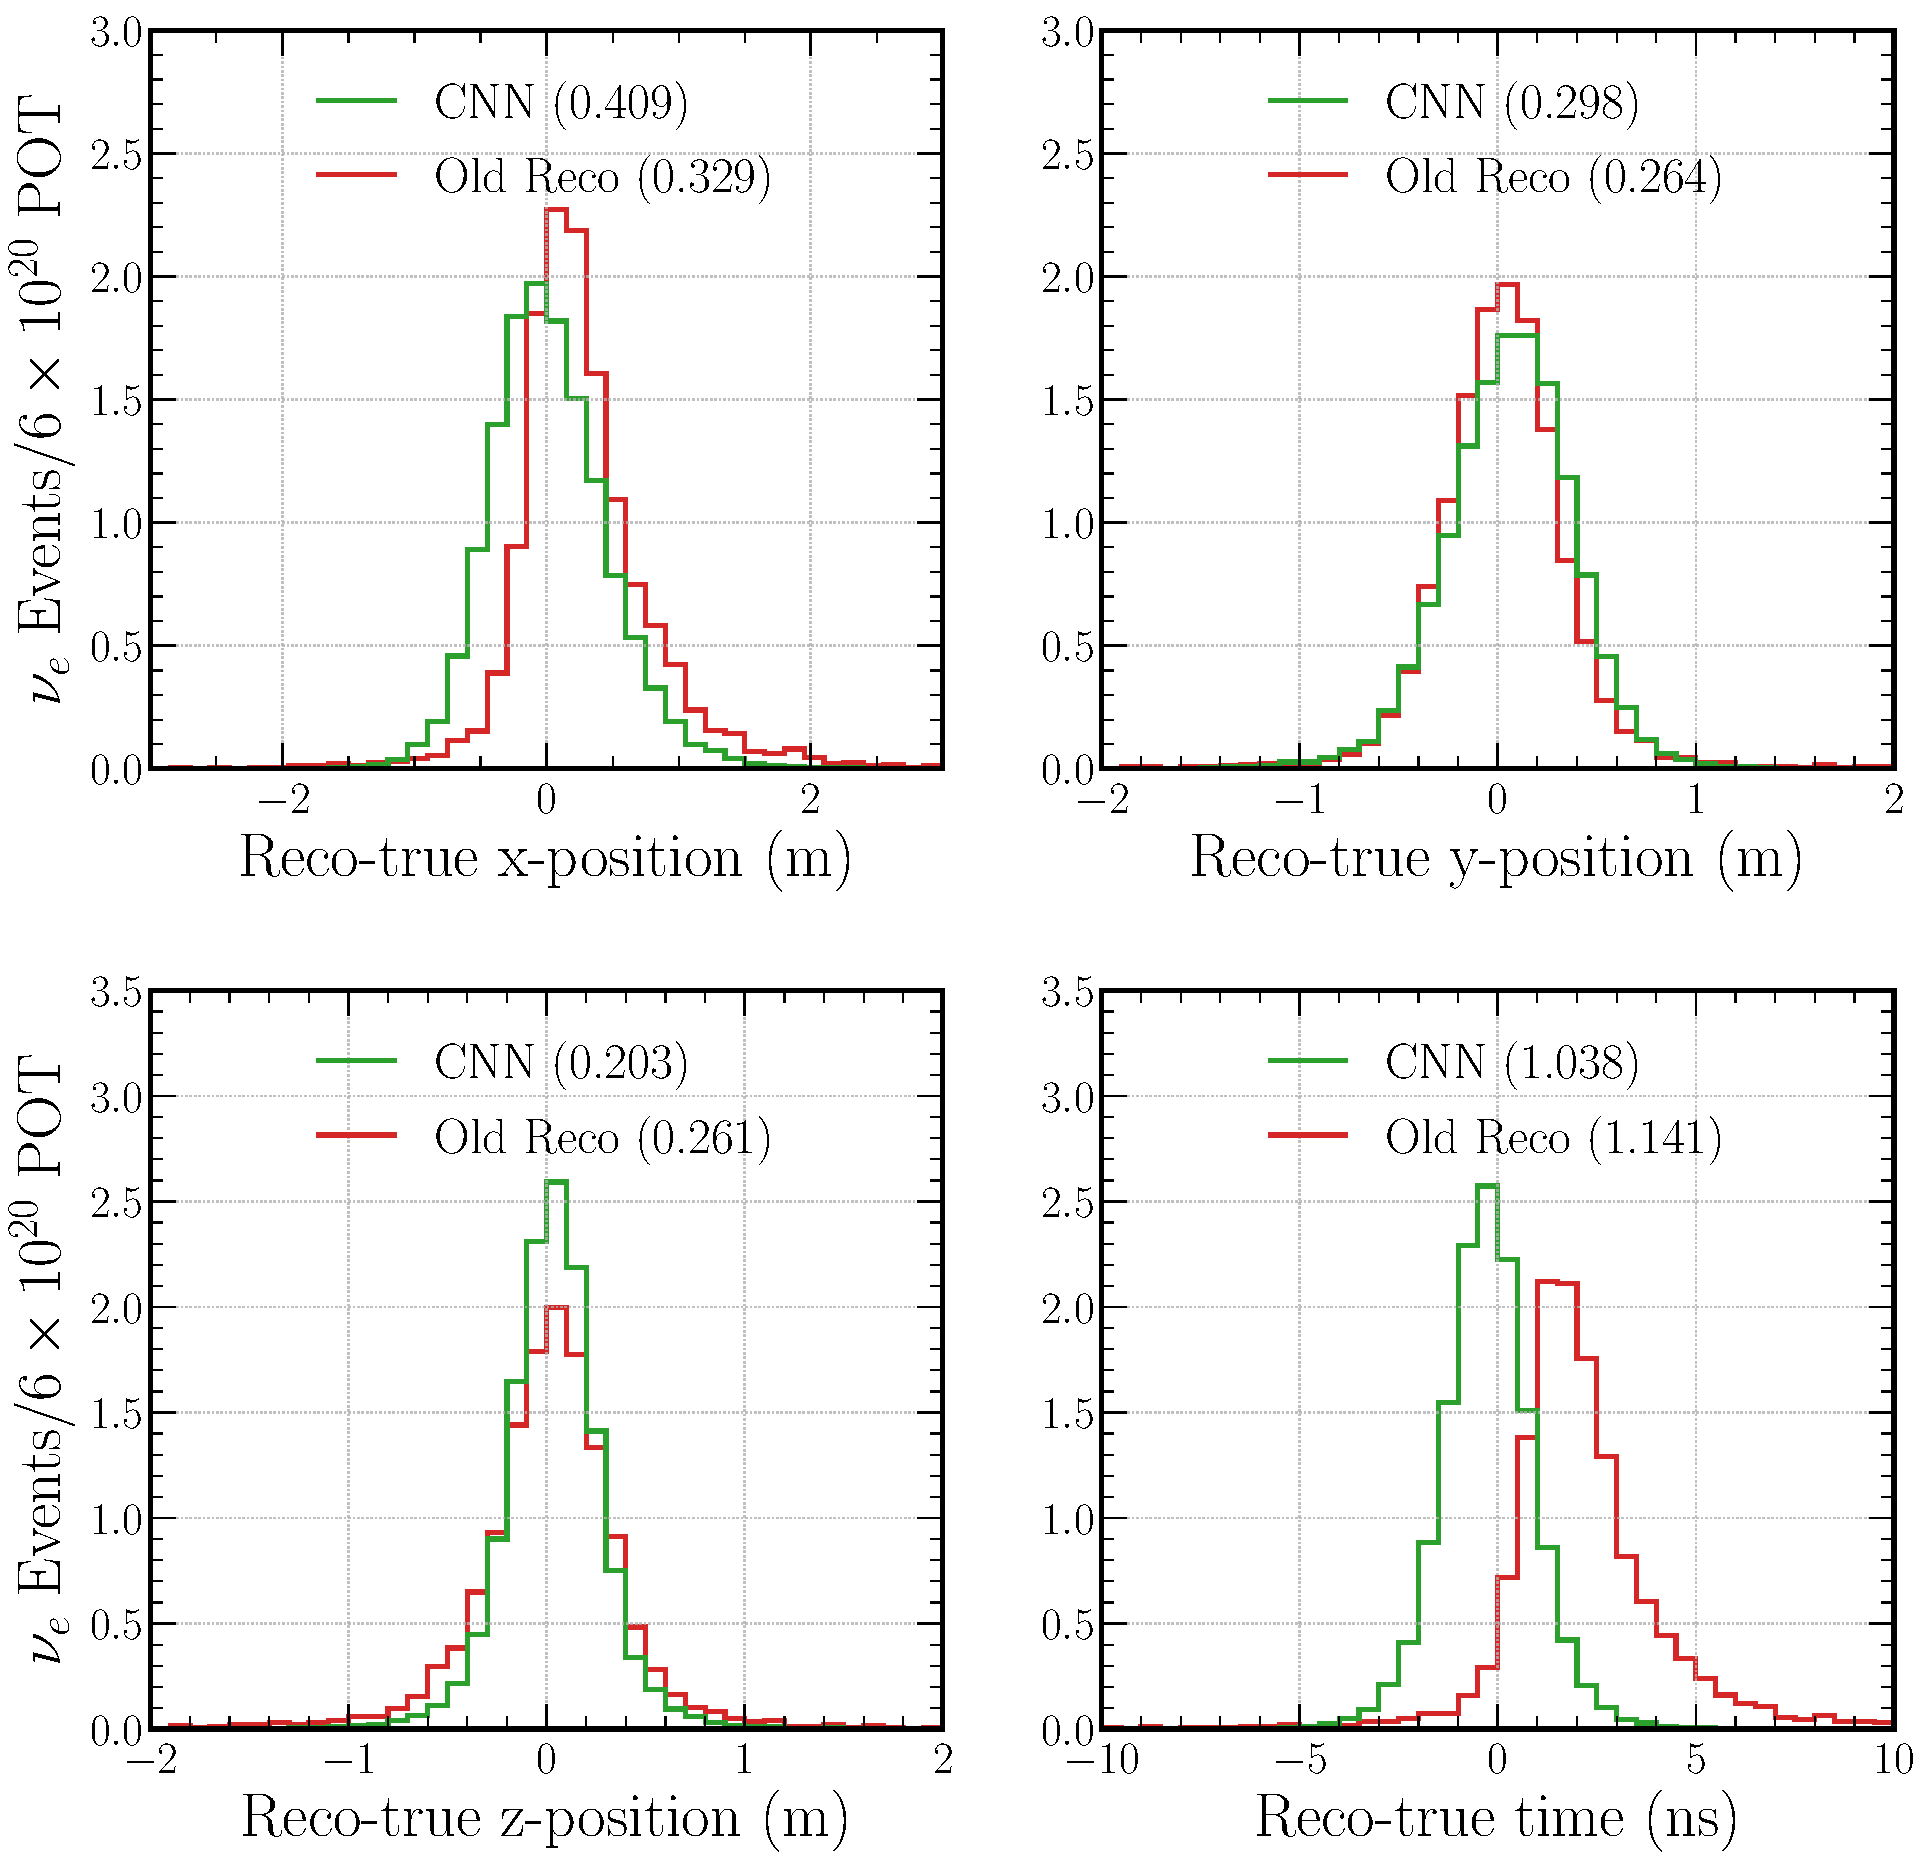
\includegraphics[width=0.9\textwidth]{diagrams/7-results/final_vertex_nuel_res_comparison.pdf}
    \caption[Reco-true distributions for the interaction vertex parameters for CC $\nu_{e}$ QEL
        events] {Reco-true distributions for the interaction vertex position components and time
        for CC $\nu_{e}$ QEL events. Both the distributions for the new CNN approach and standard
        (old) reconstruction methods are shown. The standard deviation of a gaussian fit made to
        each distribution is shown in the corresponding brackets.}
    \label{fig:final_vertex_nuel_res_comparison}
\end{figure}

\begin{figure} % FINAL VTX RES NUMU COMPARISON DIAGRAM %
    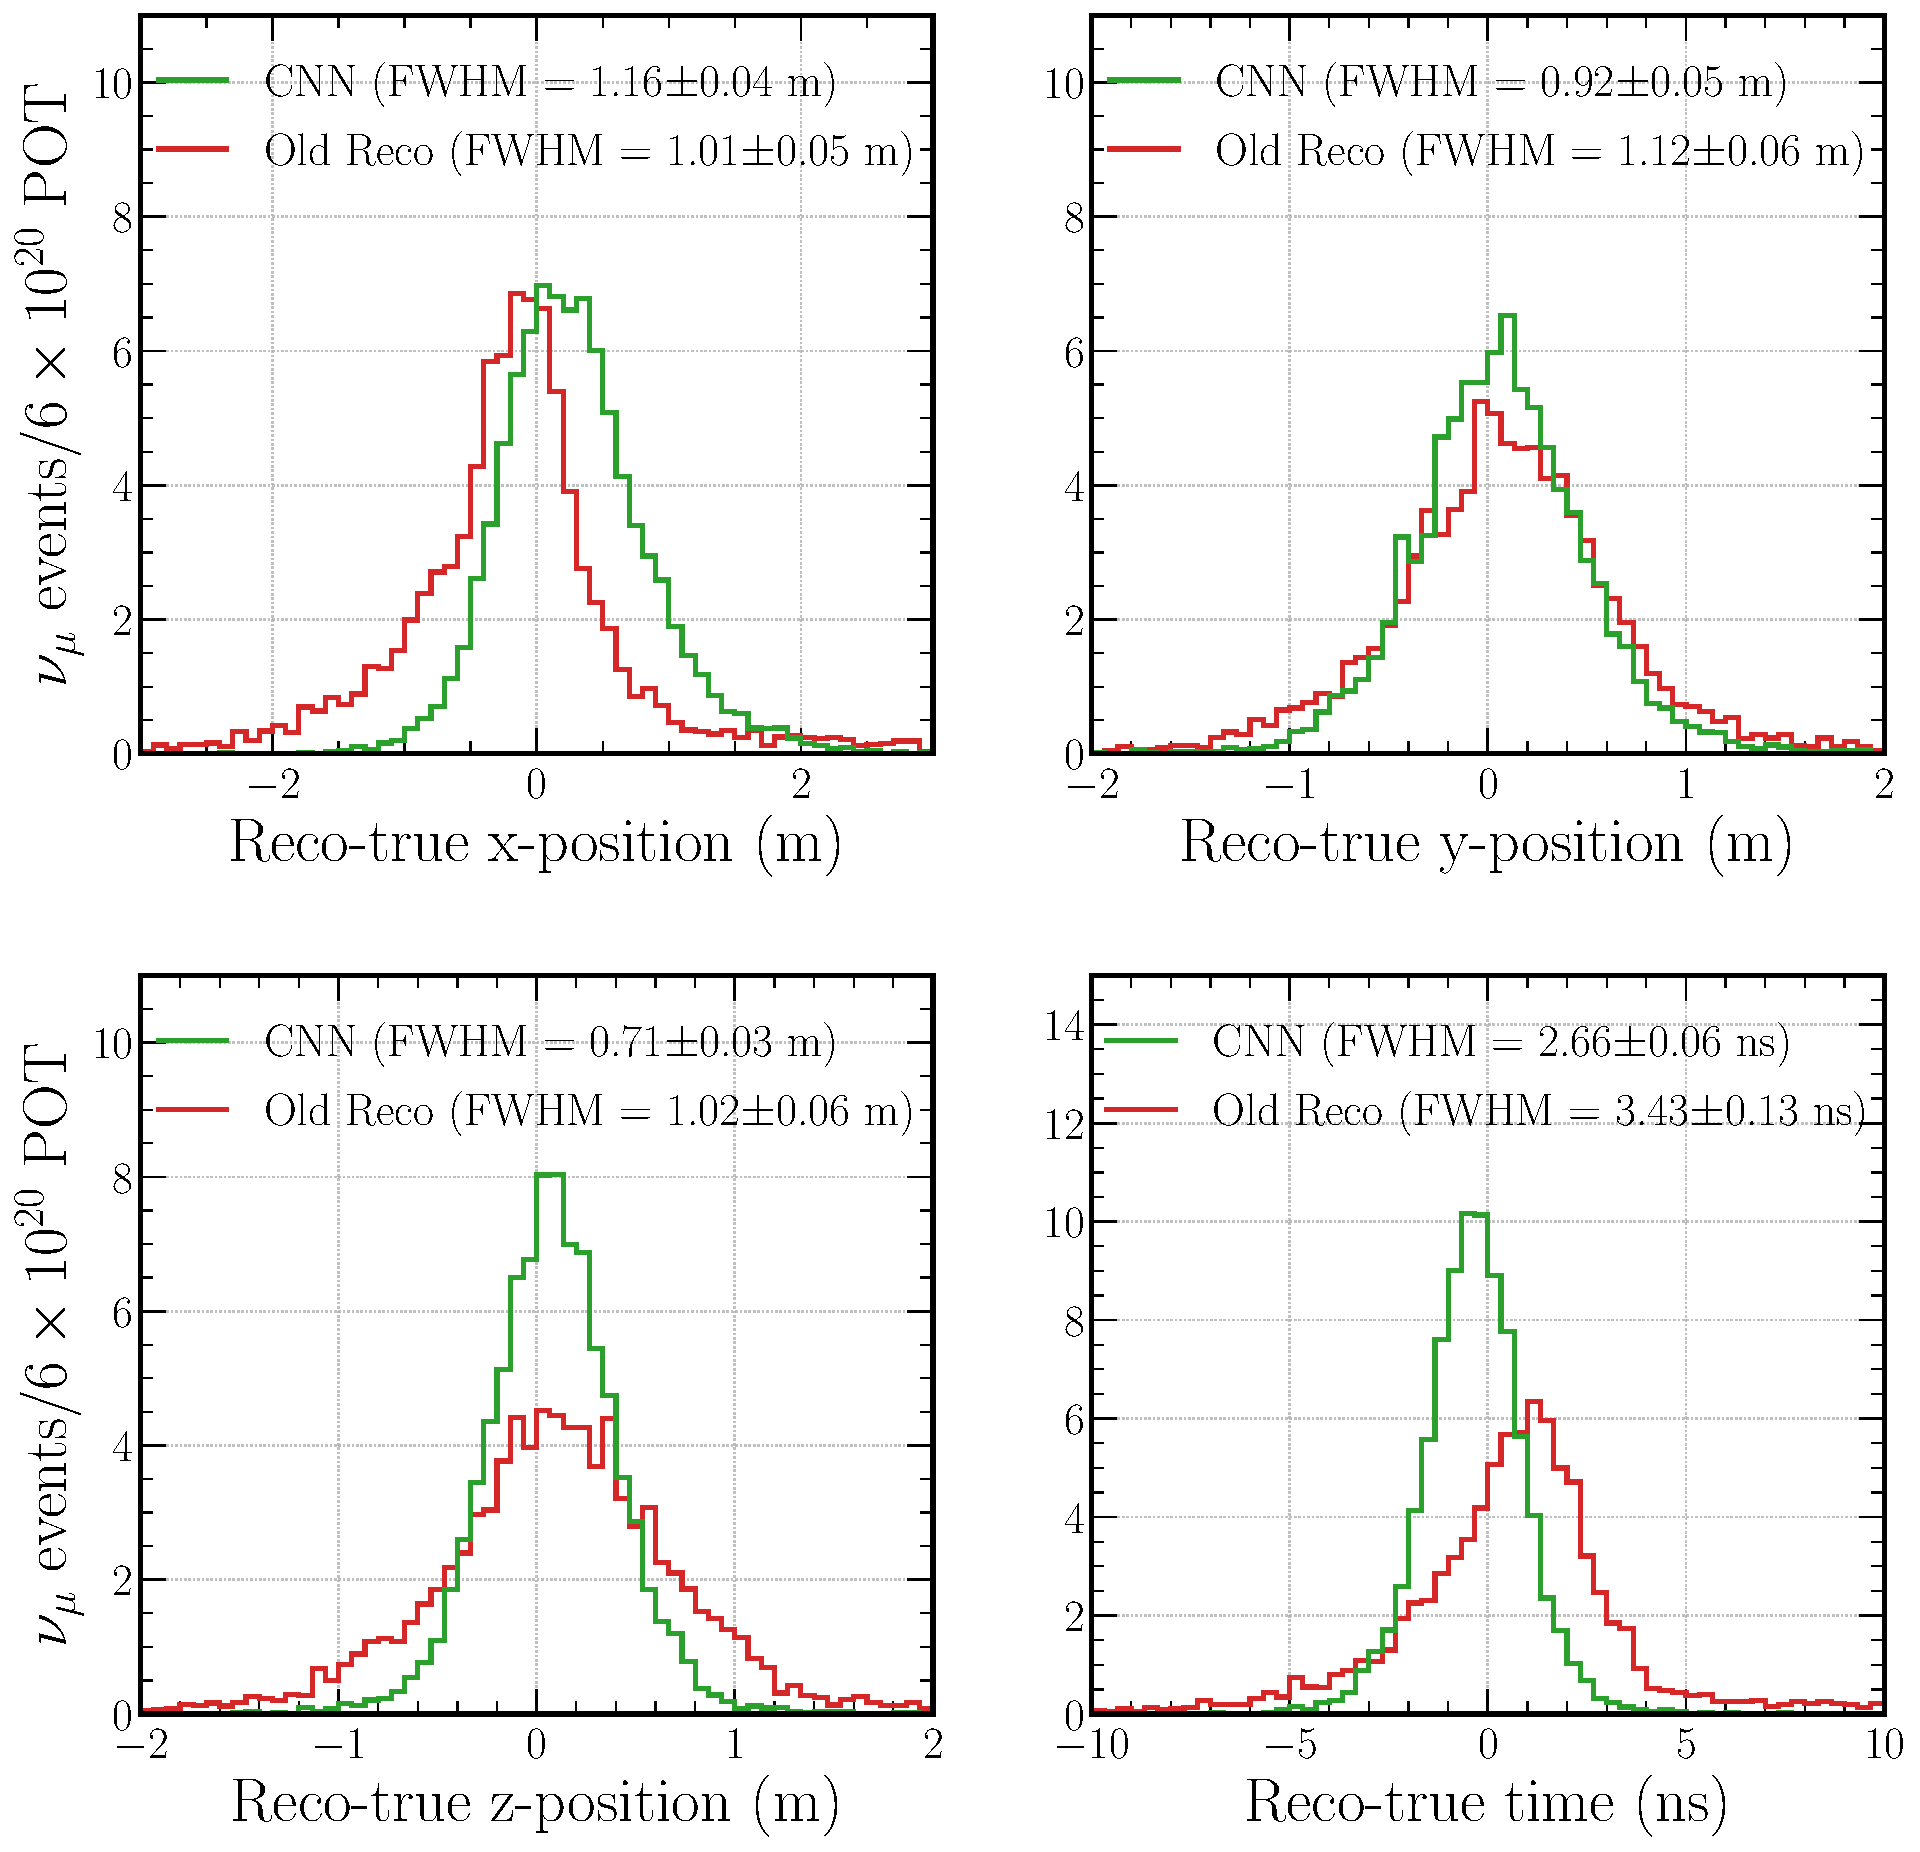
\includegraphics[width=0.9\textwidth]{diagrams/7-results/final_vertex_numu_res_comparison.pdf}
    \caption[Reco-true distributions for the interaction vertex parameters for CC $\nu_{\mu}$ QEL
        events] {Reco-true distributions for the interaction vertex position components and time
        for CC $\nu_{\mu}$ QEL events. Both the distributions for the new CNN approach and
        standard (old) reconstruction methods are shown. The standard deviation of a gaussian fit
        made to each distribution is shown in the corresponding brackets.}
    \label{fig:final_vertex_numu_res_comparison}
\end{figure}

\subsection{Combined performance} %%%%%%%%%%%%%%%%%%%%%%%%%%%%%%%%%%%%%%%%%%%%%%%%%%%%%%%%%%%%%%%%
\label{sec:results_eval_combined} %%%%%%%%%%%%%%%%%%%%%%%%%%%%%%%%%%%%%%%%%%%%%%%%%%%%%%%%%%%%%%%%

By combining CC $\nu_{e}$ and CC $\nu_{\mu}$ selections with neutrino energy estimation, the final
selected spectrum of events within \chipsfive running for a year can be estimated. These are shown
in \FigureRef{fig:final_nuel_passed_energy_dist} and \FigureRef{fig:final_numu_passed_energy_dist}
for CC $\nu_{e}$ and CC $\nu_{\mu}$ selections respectively. Although a detailed \chipsfive
sensitivity analysis is not included in this work, the expected curves for different values of
$\delta_{CP}$ are shown in the CC $\nu_{e}$ case for interest.

\begin{figure} % FINAL NUEL ENERGY DIST DIAGRAM %
    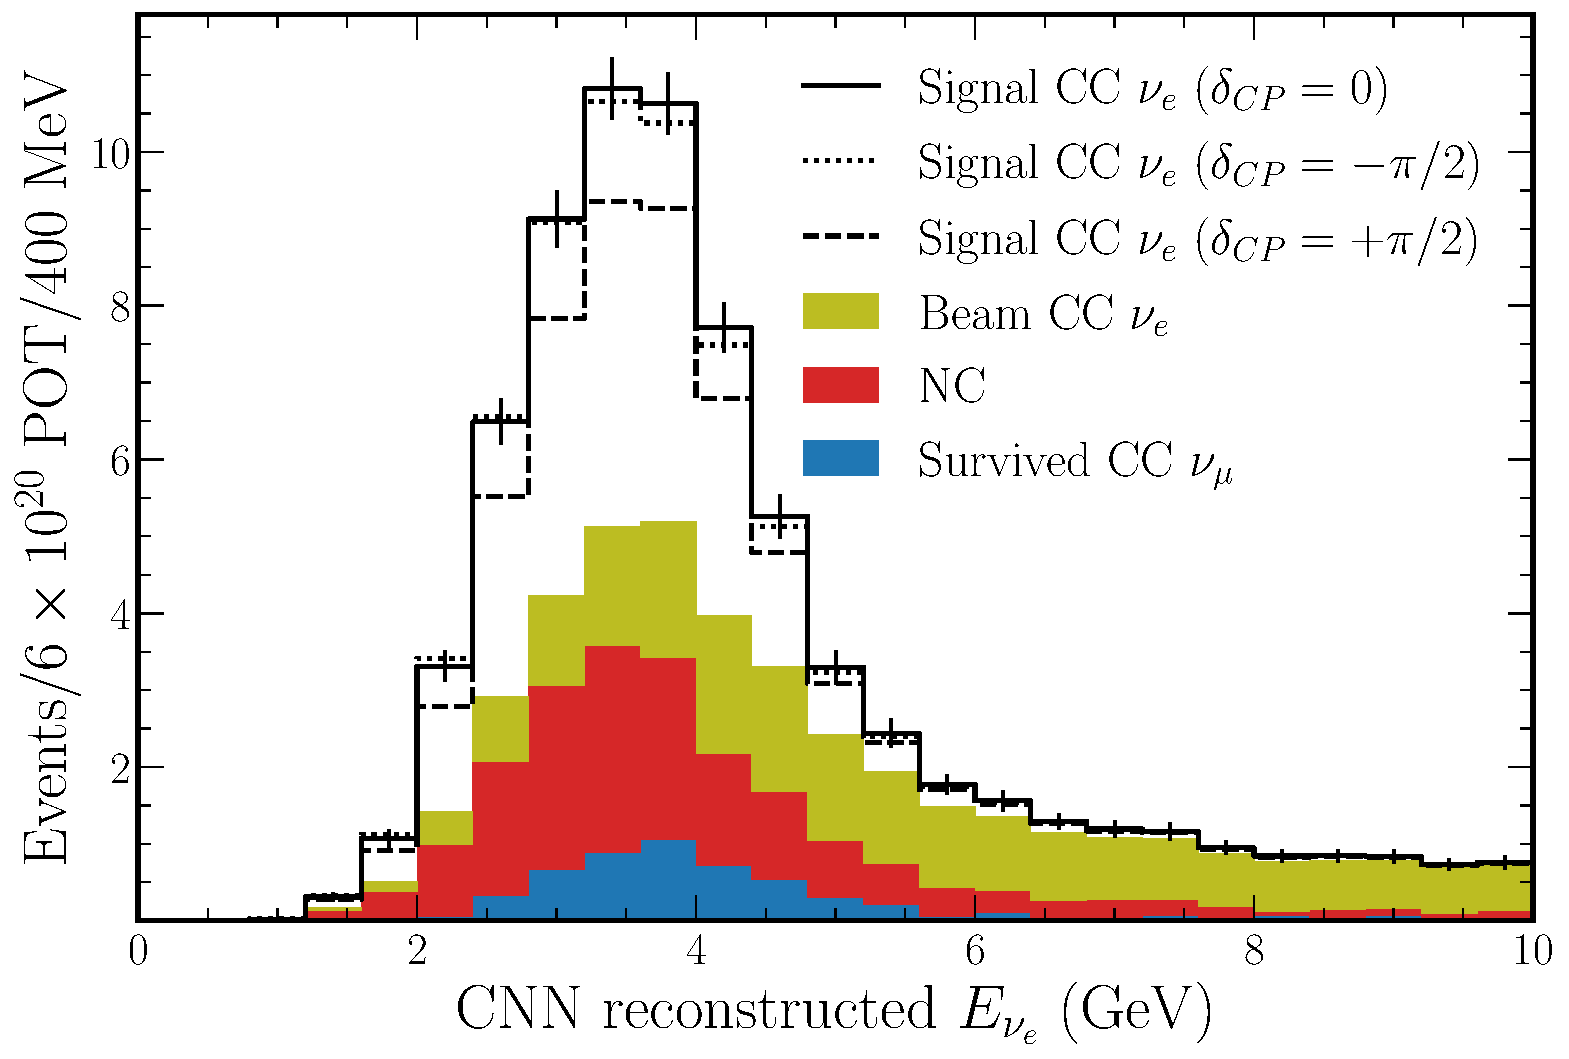
\includegraphics[width=0.8\textwidth]{diagrams/7-results/final_nuel_passed_energy_dist.pdf}
    \caption[Distribution of CNN reconstructed $\nu_{e}$ energies for CC $\nu_{e}$ selected events]
    {Distribution of CNN reconstructed $\nu_{e}$ energies for CC $\nu_{e}$ selected events. The
        appeared CC $\nu_{e}$ signal component as well as the intrinsic beam CC $\nu_{e}$, NC and
        survived CC $\nu_{\mu}$ background components are shown stacked to generate the full
        distribution. Expected totals are show in each bin for
        $\delta_{CP}=-\pi/2,~0,~\text{and}~+\pi/2$.}
    \label{fig:final_nuel_passed_energy_dist}
\end{figure}

\begin{figure} % FINAL NUMU ENERGY DIST DIAGRAM %
    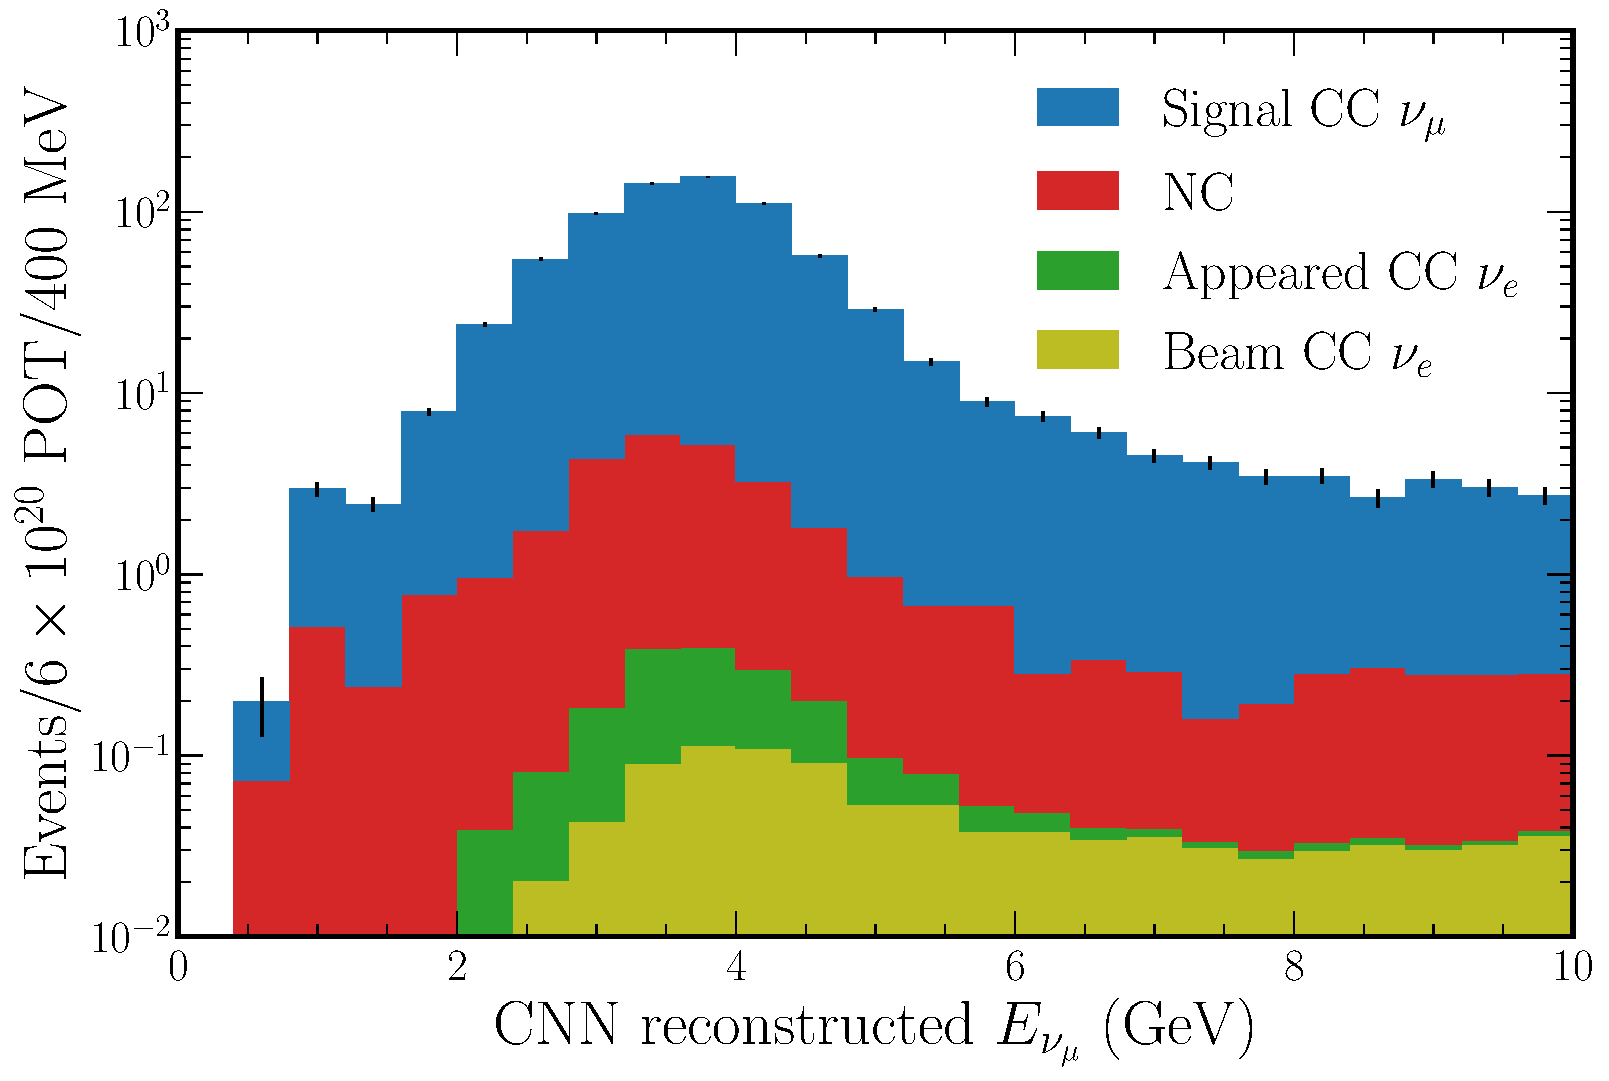
\includegraphics[width=0.8\textwidth]{diagrams/7-results/final_numu_passed_energy_dist.pdf}
    \caption[Distribution of CNN reconstructed $\nu_{\mu}$ energies for CC $\nu_{\mu}$ selected
        events] {Distribution of CNN reconstructed $\nu_{\mu}$ energies for CC $\nu_{\mu}$
        selected events. The survived CC $\nu_{\mu}$ signal component as well as the appeared CC
        $\nu_{e}$, intrinsic beam CC $\nu_{e}$, and NC background components are shown stacked to
        generate the full distribution.}
    \label{fig:final_numu_passed_energy_dist}
\end{figure}

\section{Explainability} %%%%%%%%%%%%%%%%%%%%%%%%%%%%%%%%%%%%%%%%%%%%%%%%%%%%%%%%%%%%%%%%%%%%%%%%%
\label{sec:results_explain} %%%%%%%%%%%%%%%%%%%%%%%%%%%%%%%%%%%%%%%%%%%%%%%%%%%%%%%%%%%%%%%%%%%%%%

A common and justified concern with CNNs is their tendency to be used as a black box (inputs in,
outputs out) with no understanding of their inner working. For detailed physics analyses, this can
have significant confidence implications for the final results. Although difficult quantitatively,
qualitative assessments of the trained networks can go a long way to proving they behave as
desired. Here, a sample of efforts to explain the inner workings of the trained CNNs presented in
this work are described.

\subsection{Feature map visualisation} %%%%%%%%%%%%%%%%%%%%%%%%%%%%%%%%%%%%%%%%%%%%%%%%%%%%%%%%%%%
\label{sec:results_explain_vis} %%%%%%%%%%%%%%%%%%%%%%%%%%%%%%%%%%%%%%%%%%%%%%%%%%%%%%%%%%%%%%%%%%

Visualisations of the output feature maps from the first, second, and third VGG blocks for each of
the trained networks (cosmic rejection, beam classification, and energy estimation) are shown in
\FigureRef{fig:cnn_visualisations}, using the event shown in \FigureRef{fig:explain_example_event}
as input. Learnt Cherenkov ring features are observed: ring edges, ring holes, outlying hits,
Hough peaks, and a myriad of combinations are seen. Furthermore, there are clear differences
between the specific networks, proving each network learns those features found to be important
for its tasks.

\begin{figure} % EXPLAIN EXAMPLE EVENT DIAGRAM %
    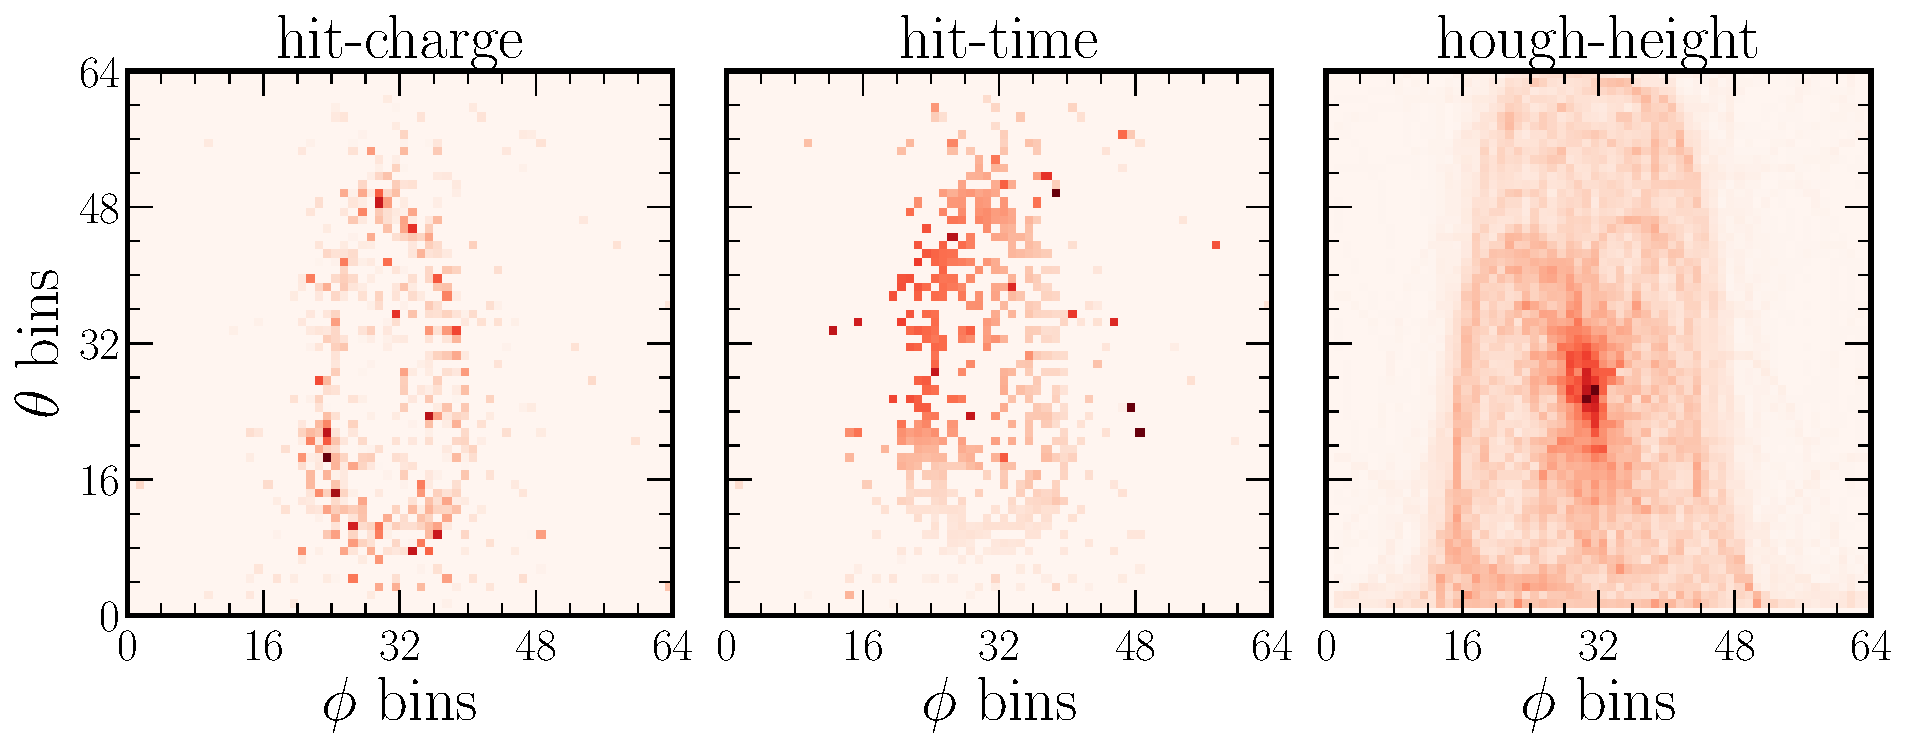
\includegraphics[width=\textwidth]{diagrams/7-results/explain_example_event.pdf}
    \caption[Example CC quasi-elastic $\nu_{e}$ event for explainability]
    {Three map representation of a CC quasi-elastic $\nu_{e}$ event. Initiated by a $\nu_{e}$ of
        energy \unit{2.4}{\GeV} with a final state $e^{-}$ of energy \unit{1.6}{\GeV}.}
    \label{fig:explain_example_event}
\end{figure}

\begin{figure} % ACTIVATIONS DIAGRAM %
    \centering
    \subcaptionbox{Cosmic rejection\label{fig:explain_cosmic_activations}}{%
        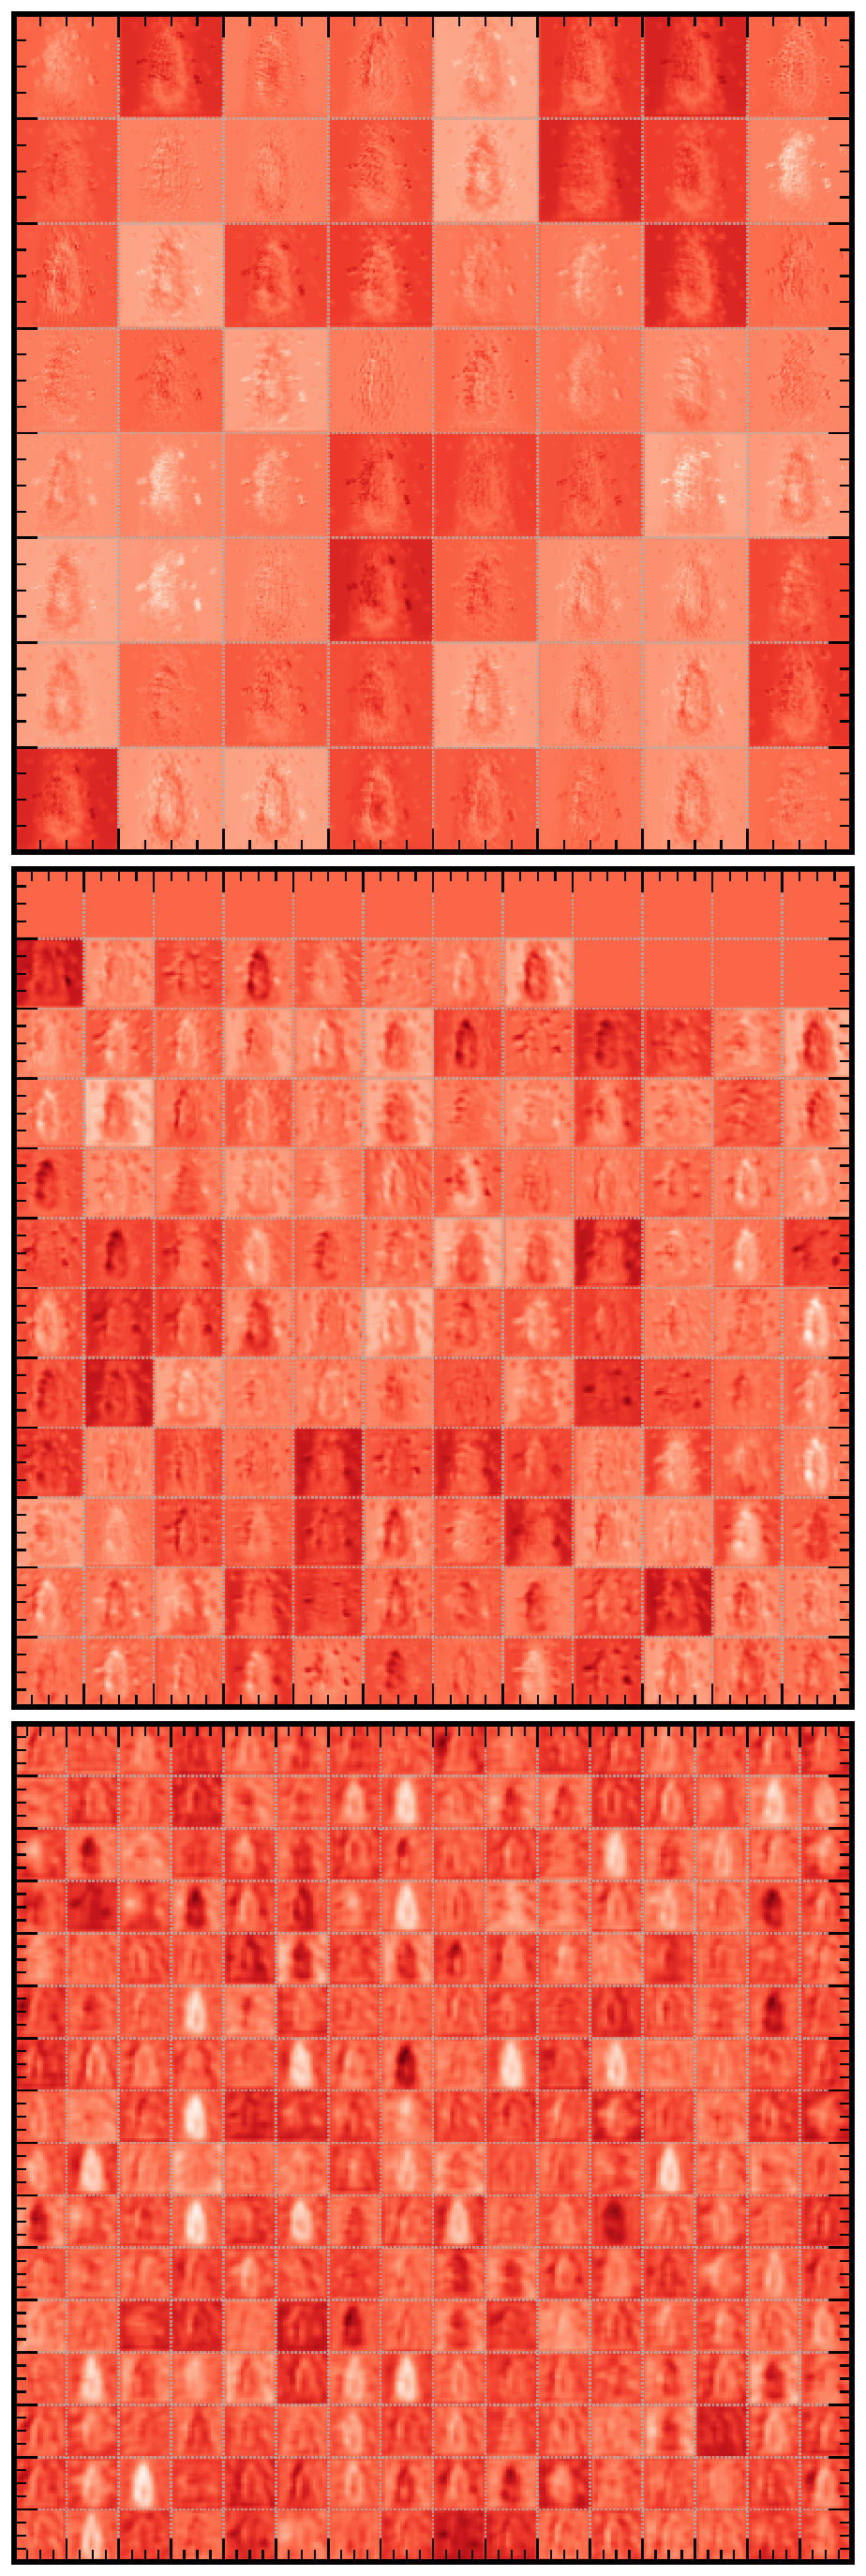
\includegraphics[height=14cm]{diagrams/7-results/explain_cosmic_activations.pdf}%
    }
    \quad
    \subcaptionbox{Beam classification\label{fig:explain_beam_activations}}{%
        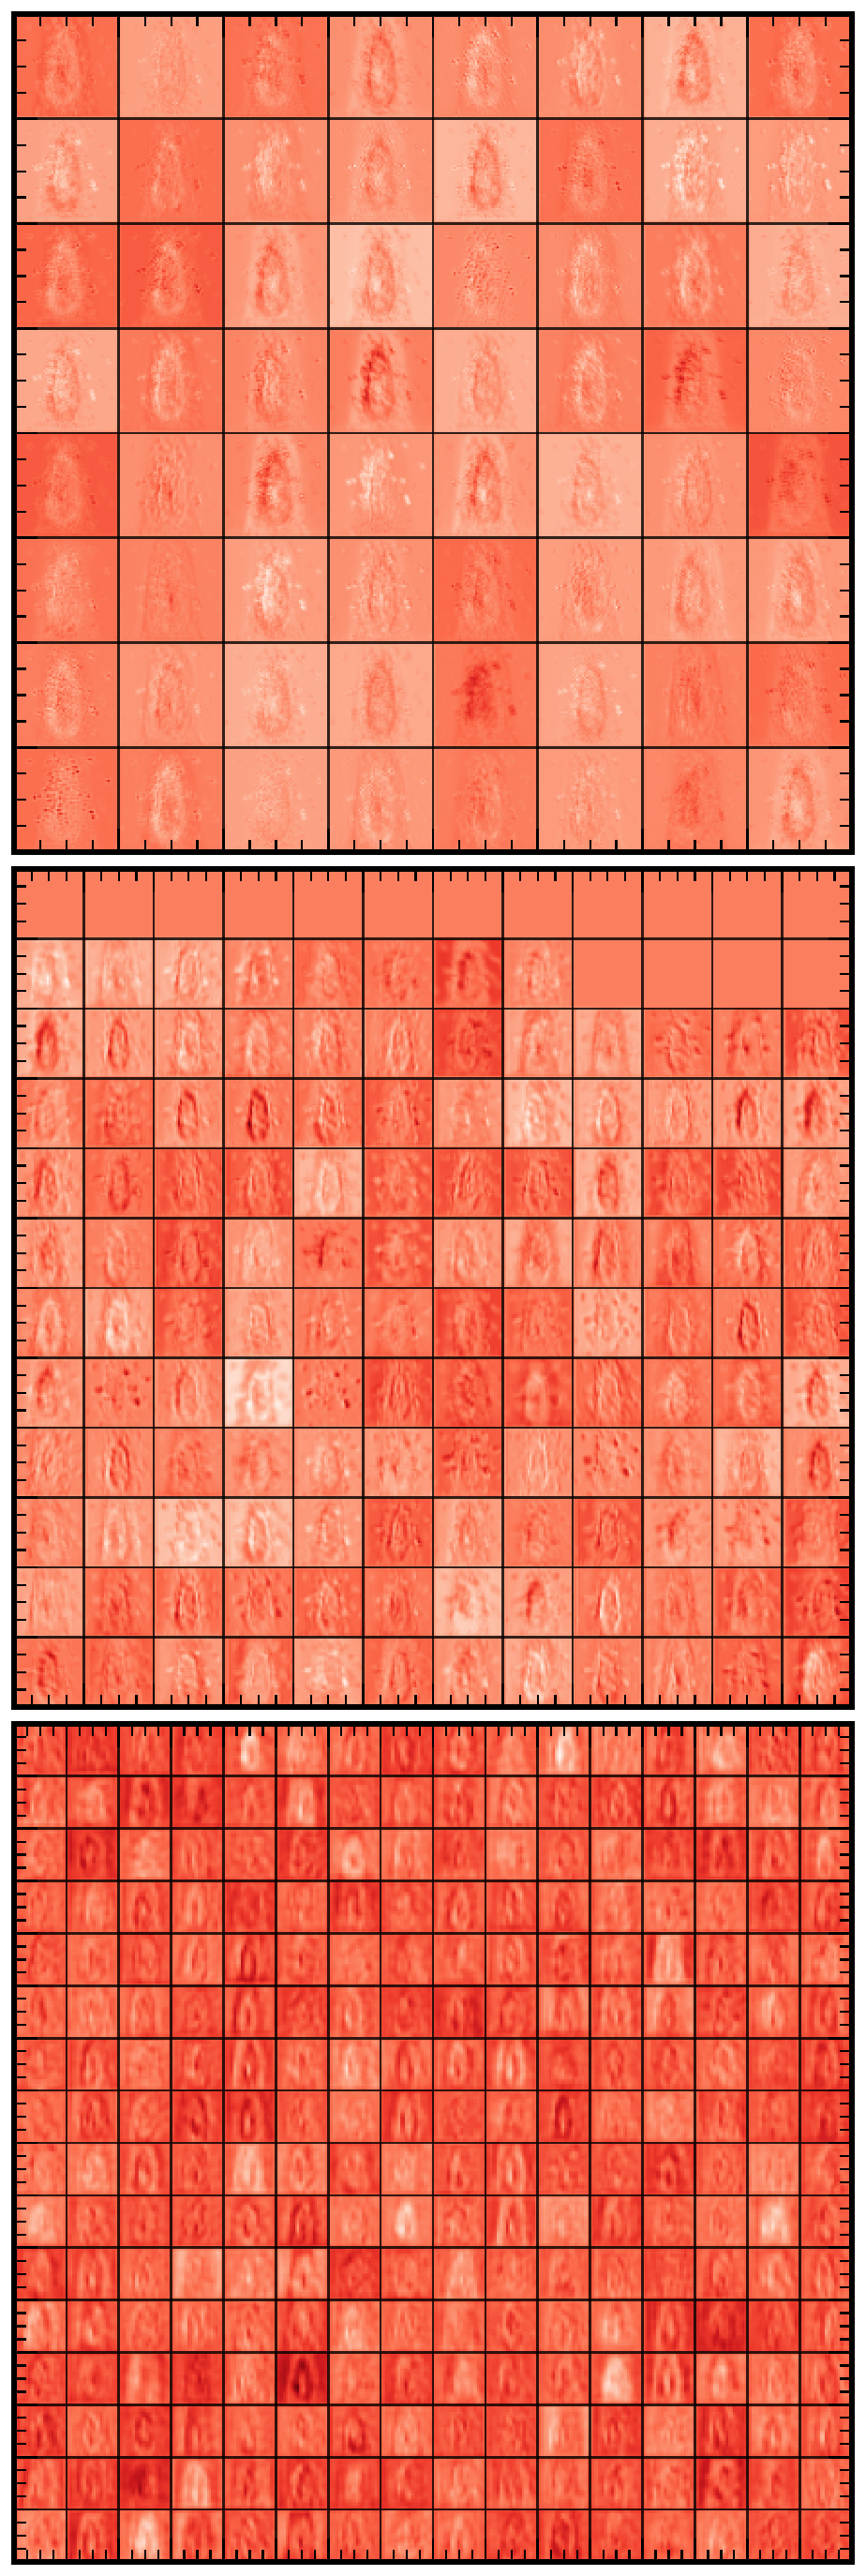
\includegraphics[height=14cm]{diagrams/7-results/explain_beam_activations.pdf}%
    }
    \quad
    \subcaptionbox{Energy estimation\label{fig:explain_energy_activations}}{%
        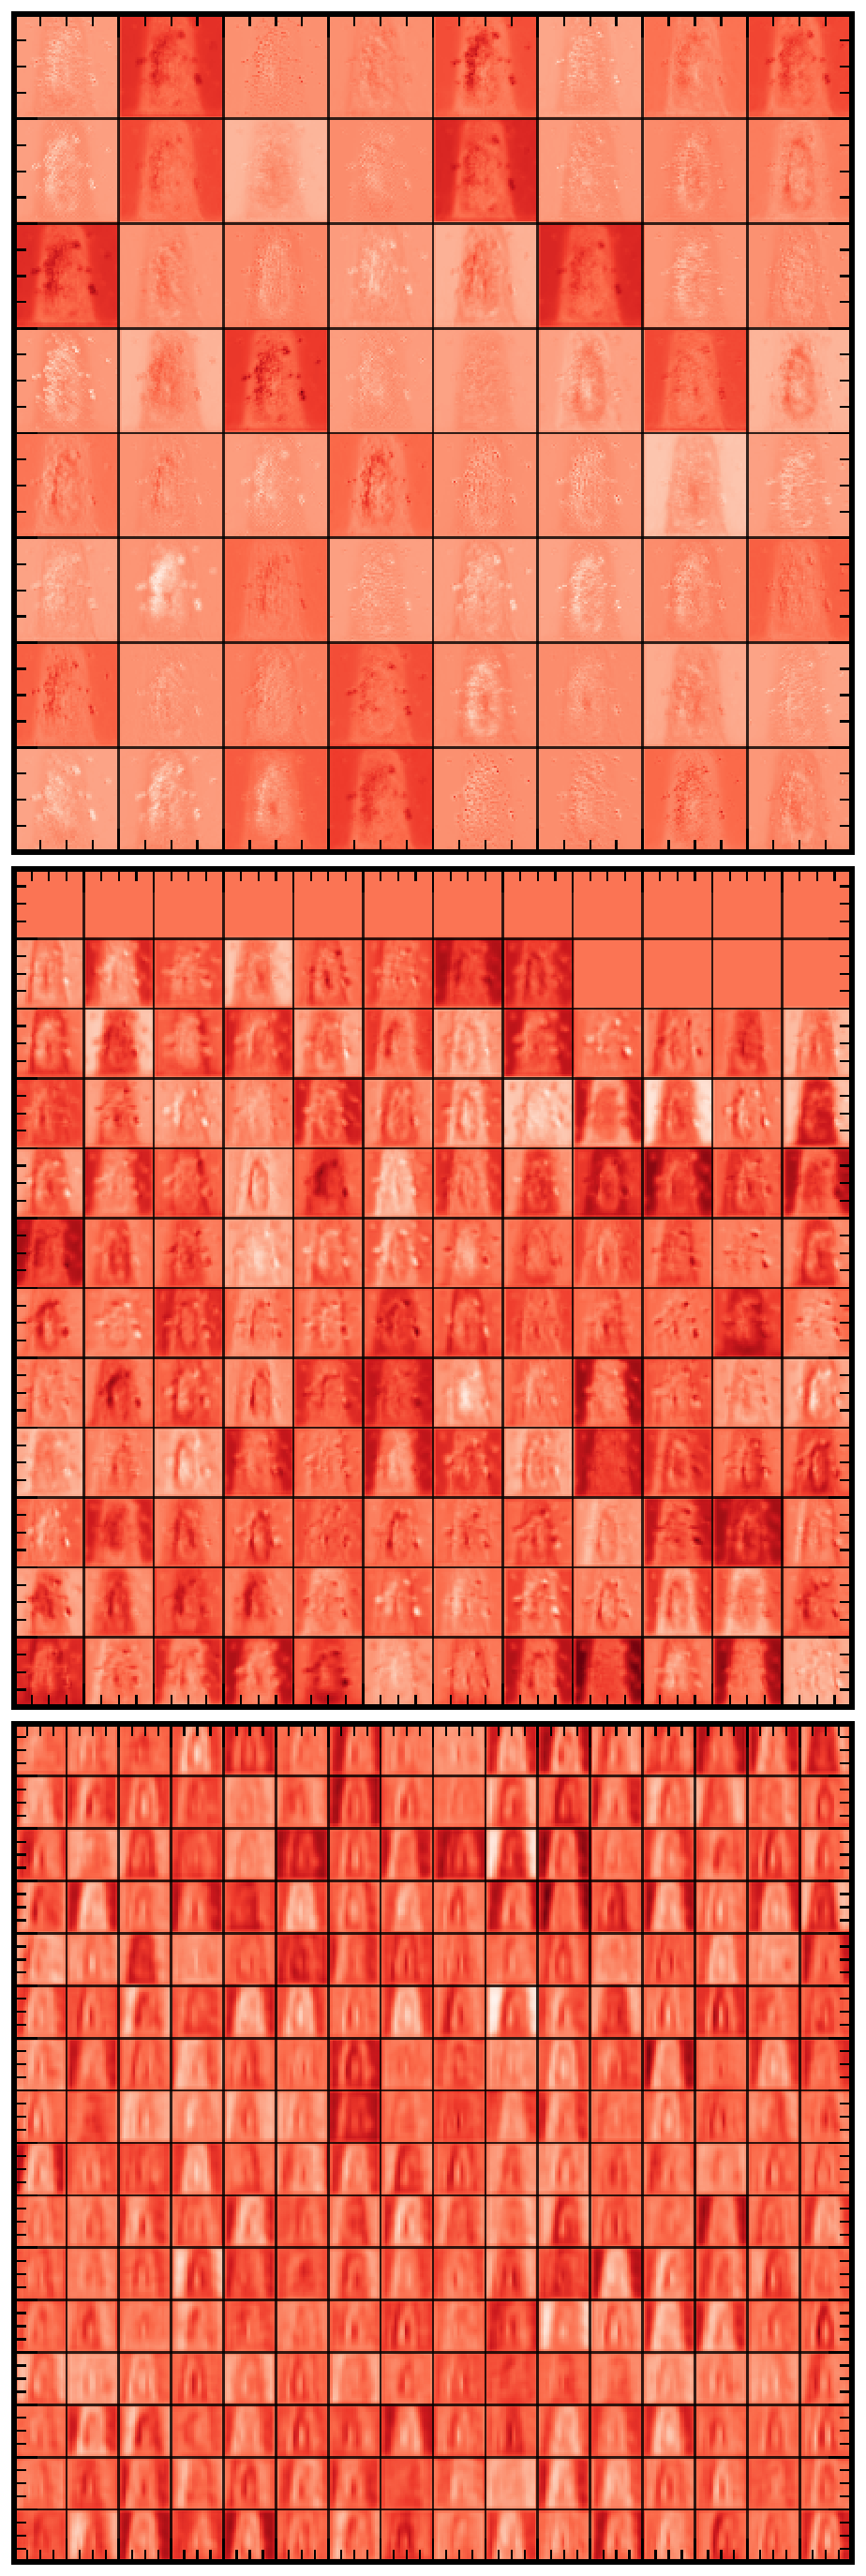
\includegraphics[height=14cm]{diagrams/7-results/explain_energy_activations.pdf}%
    }
    \caption[Visualisations of trained feature map outputs]
    {Visualisations of the feature map outputs, using as input the event shown in
        \FigureRef{fig:explain_example_event}. Shown are the activated feature map outputs from
        the first (top), the second (middle), and the third (bottom) VGG blocks for each of the
        trained network types. A chipsnet architecture with only a single branch and all three
        input event maps stacked into a single three-channel input image is used for simplicity.}
    \label{fig:cnn_visualisations}
\end{figure}

\subsection{t-SNE visualisation} %%%%%%%%%%%%%%%%%%%%%%%%%%%%%%%%%%%%%%%%%%%%%%%%%%%%%%%%%%%%%%%%%
\label{sec:results_explain_tsne} %%%%%%%%%%%%%%%%%%%%%%%%%%%%%%%%%%%%%%%%%%%%%%%%%%%%%%%%%%%%%%%%%

Another technique to analyse trained CNNs is t-Distributed Stochastic Neighbour Embedding
(t-SNE)~\cite{maaten2008}. The t-SNE procedure is an unsupervised learning algorithm to visualise
the learnt high-dimensional feature-space of a trained network in a lower number of dimensions. It
accomplishes this by clustering events with similar features nearby in two-dimensional space and
separating events with dissimilar features. Here, the outputs from the last fully connected layer
before the output layer (with 512 dimensions) are used as input, as they provide the final
representation of the learnt network features.

Visualisations of the t-SNE algorithm outputs, when applied to both the trained cosmic rejection
and beam classification networks, are shown in \FigureRef{fig:explain_cosmic_tsne} and
\FigureRef{fig:explain_beam_tsne}, respectively. The very strong cosmic like to beam like
separation presented in \SectionRef{sec:results_eval_cosmic} is clear from the cosmic rejection
visualisation. Conversely, for the beam classification network, the separation is weaker, with
major overlap between categories, especially for CC $\nu_{e}$ and NC events.

\begin{figure} % COSMIC t-SNE DIAGRAM %
    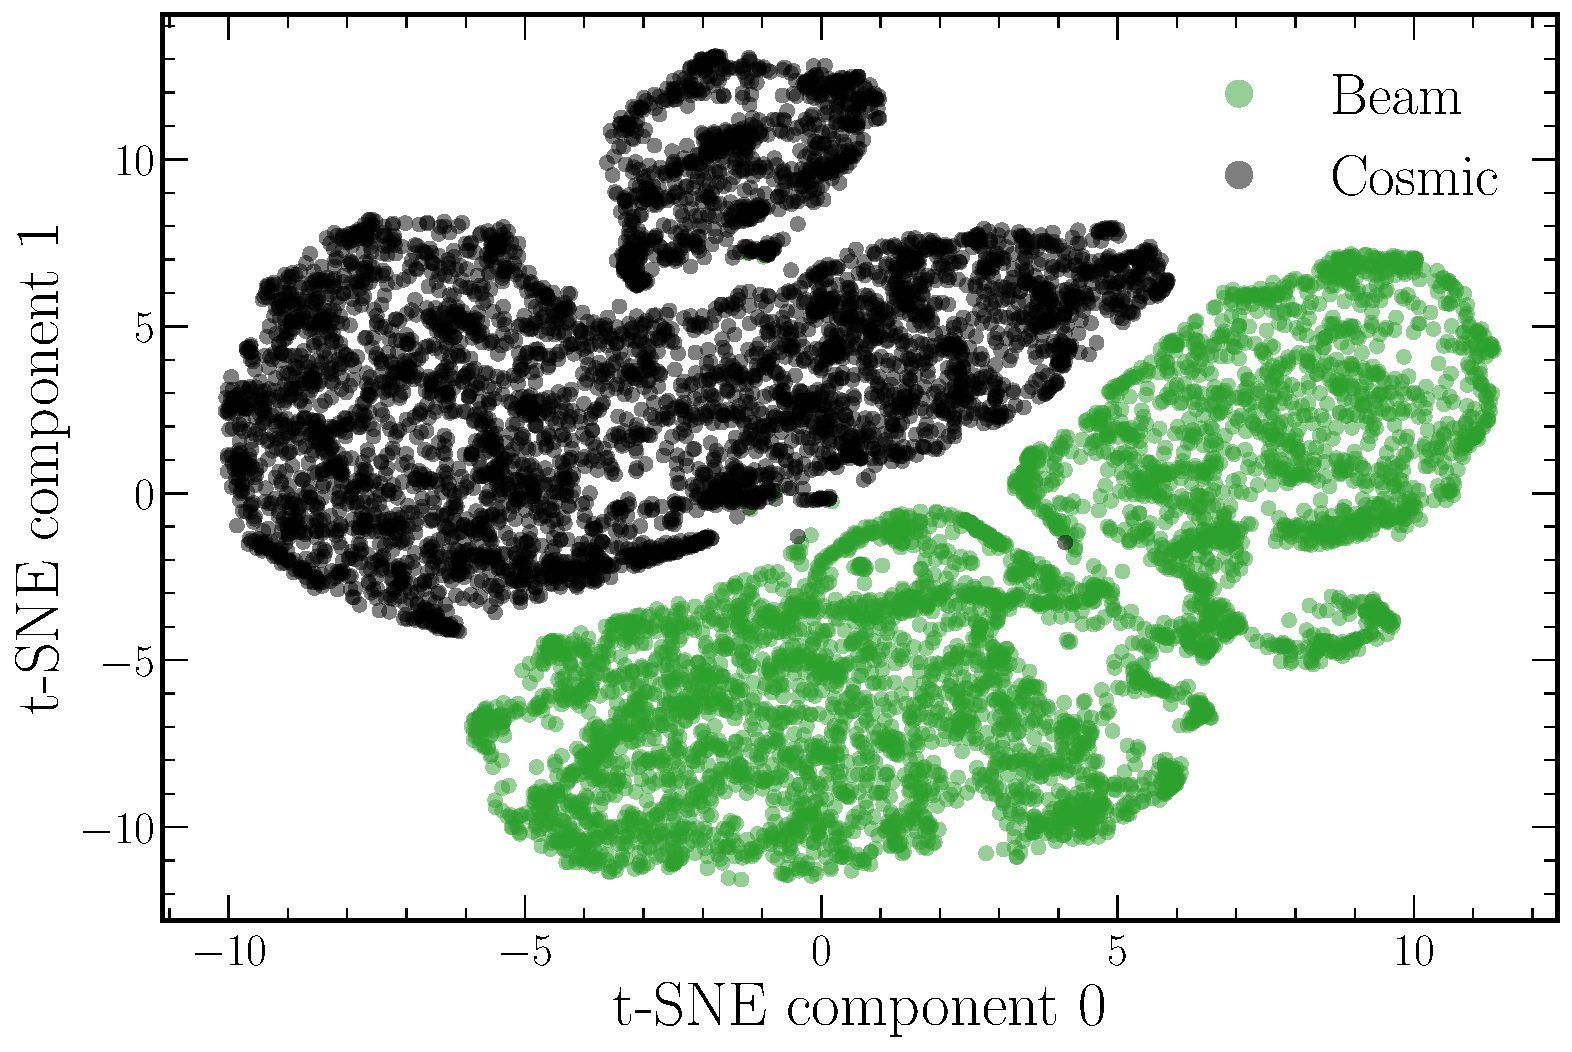
\includegraphics[width=\textwidth]{diagrams/7-results/explain_cosmic_tsne.pdf}
    \caption[Cosmic rejection network output t-SNE space]
    {Two dimensional probability space of beam and cosmic events generated using the t-SNE
        procedure on the final fully-connected layer of the trained cosmic rejection network.}
    \label{fig:explain_cosmic_tsne}
\end{figure}

\begin{figure} % BEAM t-SNE DIAGRAM %
    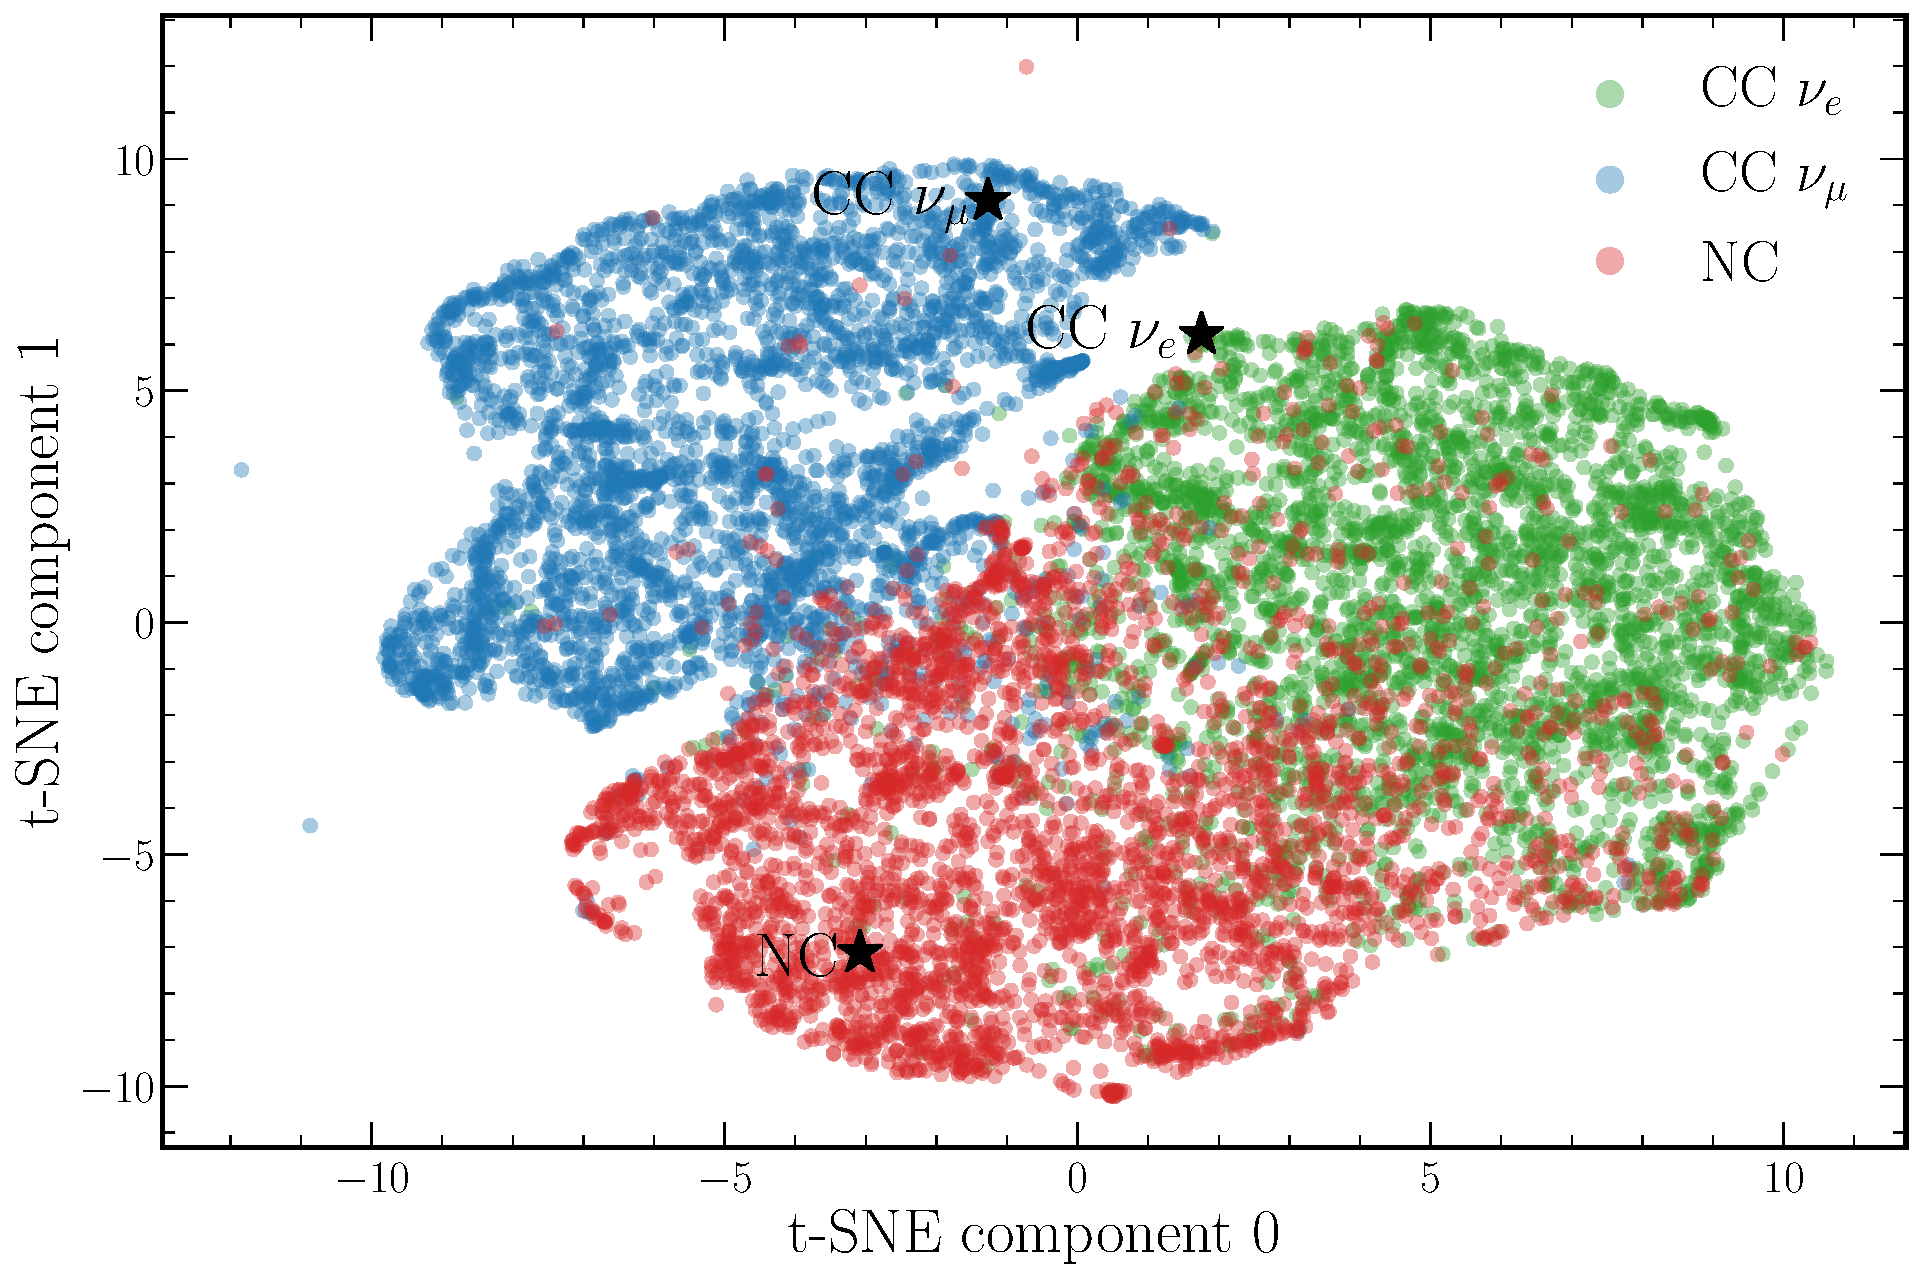
\includegraphics[width=\textwidth]{diagrams/7-results/explain_beam_tsne.pdf}
    \caption[Beam classification network output t-SNE space]
    {Two dimensional probability space of different beam events generated using the t-SNE
        procedure on the final fully-connected layer of the trained beam classification network.
        Three events, one highly CC $\nu_{e}$ like, one highly CC $\nu_{\mu}$ like, and one highly
        NC like are highlighted and shown in \FigureRef{fig:explain_beam_tsne_events}.}
    \label{fig:explain_beam_tsne}
\end{figure}

For the beam classification network, three events, labelled in the t-SNE space of
\FigureRef{fig:explain_beam_tsne}, are shown in \FigureRef{fig:explain_beam_tsne_events}. Each
event is highly representative of its class, achieving a high respective \emph{combined category}
score. Both the CC $\nu_{e}$ and NC events are typical of that expected. However, the CC
$\nu_{\mu}$ event contains a primary charged lepton that escapes the detector volume, identified
by the central peak. This topology suggests that strongly classified CC $\nu_{\mu}$ events can be
identified by this `escaping' feature rather than the shape of the muon ring. Future work,
therefore, should explore using only fully contained events during beam classification training.

\begin{figure} % BEAM t-SNE EVENTS DIAGRAM %
    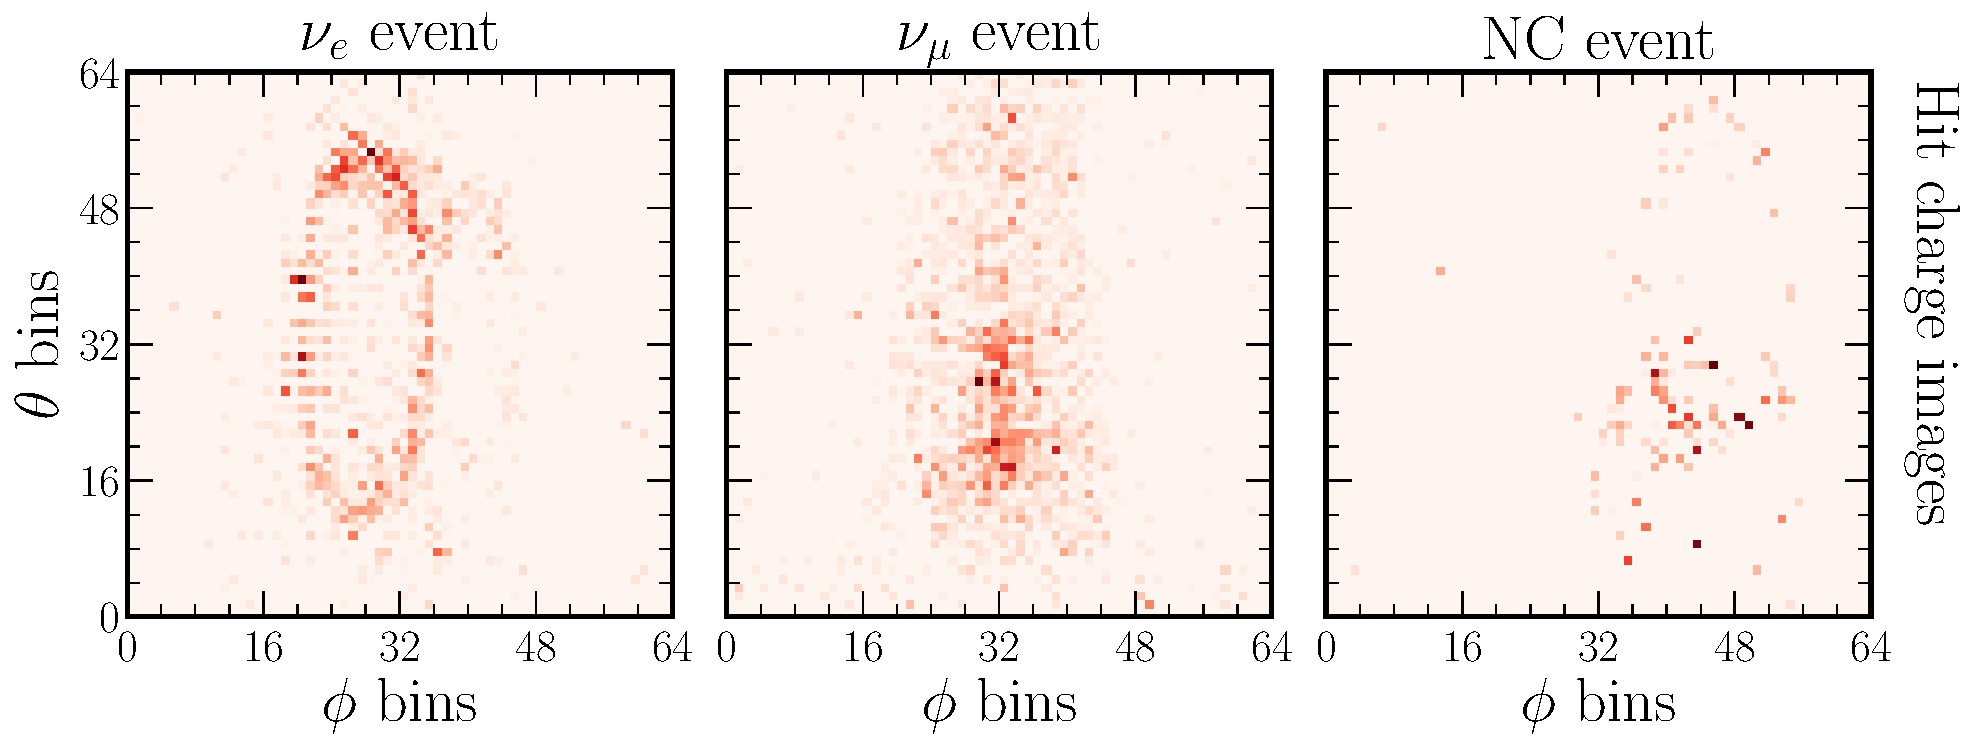
\includegraphics[width=\textwidth]{diagrams/7-results/explain_beam_tsne_events.pdf}
    \caption[Hit-charge maps of highly CC $\nu_{e}$ like, CC $\nu_{\mu}$ like, and NC like events]
    {Hit-charge maps of the highly CC $\nu_{e}$ like, CC $\nu_{\mu}$ like, and NC like events from
        \FigureRef{fig:explain_beam_tsne}.}
    \label{fig:explain_beam_tsne_events}
\end{figure}

\section{Robustness} %%%%%%%%%%%%%%%%%%%%%%%%%%%%%%%%%%%%%%%%%%%%%%%%%%%%%%%%%%%%%%%%%%%%%%%%%%%%%
\label{sec:results_robust} %%%%%%%%%%%%%%%%%%%%%%%%%%%%%%%%%%%%%%%%%%%%%%%%%%%%%%%%%%%%%%%%%%%%%%%

Recent CNN research has focused on another concern; they tend to not generalise well under
distributional changes within the input data~\cite{djolonga2020}. As the CNNs presented in this
work are trained and evaluated on simulated Monte Carlo events, this effect is of particular
relevance. If the neutrino events used differ from those measured by the real \chipsfive detector,
the network outputs may not be reliable. An effective calibration procedure and simulation
improvements can ensure any discrepancy is minimised; however, a small distributional difference
is inevitable.

Studies are presented here to prove the robustness of the trained CNNs to such changes within the
input. Broadly, the CNN inputs can be characterised as being dependent on three sets of PMT
information: the hit times, the hit charges, and the hit positions. An accurate PMT position is
deemed unimportant to the trained networks as the $64 \times 64$ input grid roughly corresponds to
bins of size \unit{2.5}{\text{m}} in $\theta$ by \unit{2.0}{\text{m}} in $\phi$ within the
\chipsfive detector. As this binning is much larger than the actual distance between PMTs,
resolving individual PMTs becomes impossible. Consequently, changes in only the PMT hit times and
hit charges are considered in three studies: the smearing of hit times, the smearing and shifting
of hit charges, and the addition of random noise.

Five classification performance metrics are used for comparison during this section and the next
(\SectionRef{sec:results_alt}):
\begin{enumerate}
    \item \textbf{Max FOM:} The optimised figure-of-merit ($\text{efficiency}\times\text{purity}$)
          value. As the FOM is proportional to $s/\sqrt{s+b}$ which increases linearly with
          detector exposure, an improvement in the FOM value linearly decreases the exposure time
          required to reach the same physics sensitivity.
    \item \textbf{High Score Eff (Pur):} The CC $\nu_{e}$ selection efficiency (purity) using the
          simple highest-scoring output neuron classification methodology. The simple
          classification strategy is used here instead of the FOM selection as it is less
          susceptible to trading off between efficiency and purity, making for easier comparison.
    \item \textbf{ROC Integral:} The area under the Receiver Operating Characteristic (ROC) curve;
          a standard tool for classification performance comparison. The curve corresponds to the
          signal CC $\nu_{e}$ efficiency plotted against the background efficiency as the CC
          $\nu_{e}$ score cut value is varied. A curve which reaches closer to the top-left (high
          signal efficiency, low background efficiency) signifies a stronger classification
          performance. An example ROC curve is shown for the smearing of hit times in
          \FigureRef{fig:calib_time_nuel_comp_curves}.
    \item \textbf{PR Integral:} The area under the Precision-Recall (PR) curve; another standard
          tool for classification performance comparison. The curve corresponds to the signal CC
          $\nu_{e}$ purity plotted against the signal efficiency as the CC $\nu_{e}$ score cut
          value is varied. A curve closer to the top-right (high signal purity, high signal
          efficiency) signifies a stronger classification performance. For imbalanced class
          frequencies such as those expected within the \chipsfive detector, the PR curve is seen
          as a more reliable indicator of performance than the ROC curve~\cite{saito2015}. An
          example PR curve is shown for the smearing of hit times in
          \FigureRef{fig:calib_time_nuel_comp_curves}.
\end{enumerate}

\subsection{Time smearing} %%%%%%%%%%%%%%%%%%%%%%%%%%%%%%%%%%%%%%%%%%%%%%%%%%%%%%%%%%%%%%%%%%%%%%%
\label{sec:results_robust_time} %%%%%%%%%%%%%%%%%%%%%%%%%%%%%%%%%%%%%%%%%%%%%%%%%%%%%%%%%%%%%%%%%%

The smearing of input hit times is found to produce a minimal reduction in output performance. For
every event, each hit-time bin for which there is an entry not equal to zero is smeared using an
absolute time randomly generated using a normal distribution with a mean of zero and a standard
deviation of $\sigma$ nanoseconds. The cases when $\sigma=0~\text{ns}$ (no smearing),
$\sigma=2~\text{ns}$, and $\sigma=5~\text{ns}$ are considered. The actual smearing values used are
scaled to the zero to one input range, and any post smearing out-of-range values are clipped to
the range boundaries.

For each case of $\sigma$, the resulting efficiency, purity, and their product (the FOM) for CC
$\nu_{e}$ events as a function of selecting events above a particular CC $\nu_{e}$ score is shown
in \FigureRef{fig:calib_time_nuel_eff_curves}. The classification performance metrics are
presented in \TableRef{tab:calib_time} with the ROC and PR curves shown in
\FigureRef{fig:calib_time_nuel_comp_curves}. Cosmic rejection and energy estimation performance
are not presented, as the resulting output changes are negligible.

\begin{figure} % CALIB TIME NUEL EFF CURVES DIAGRAM %
    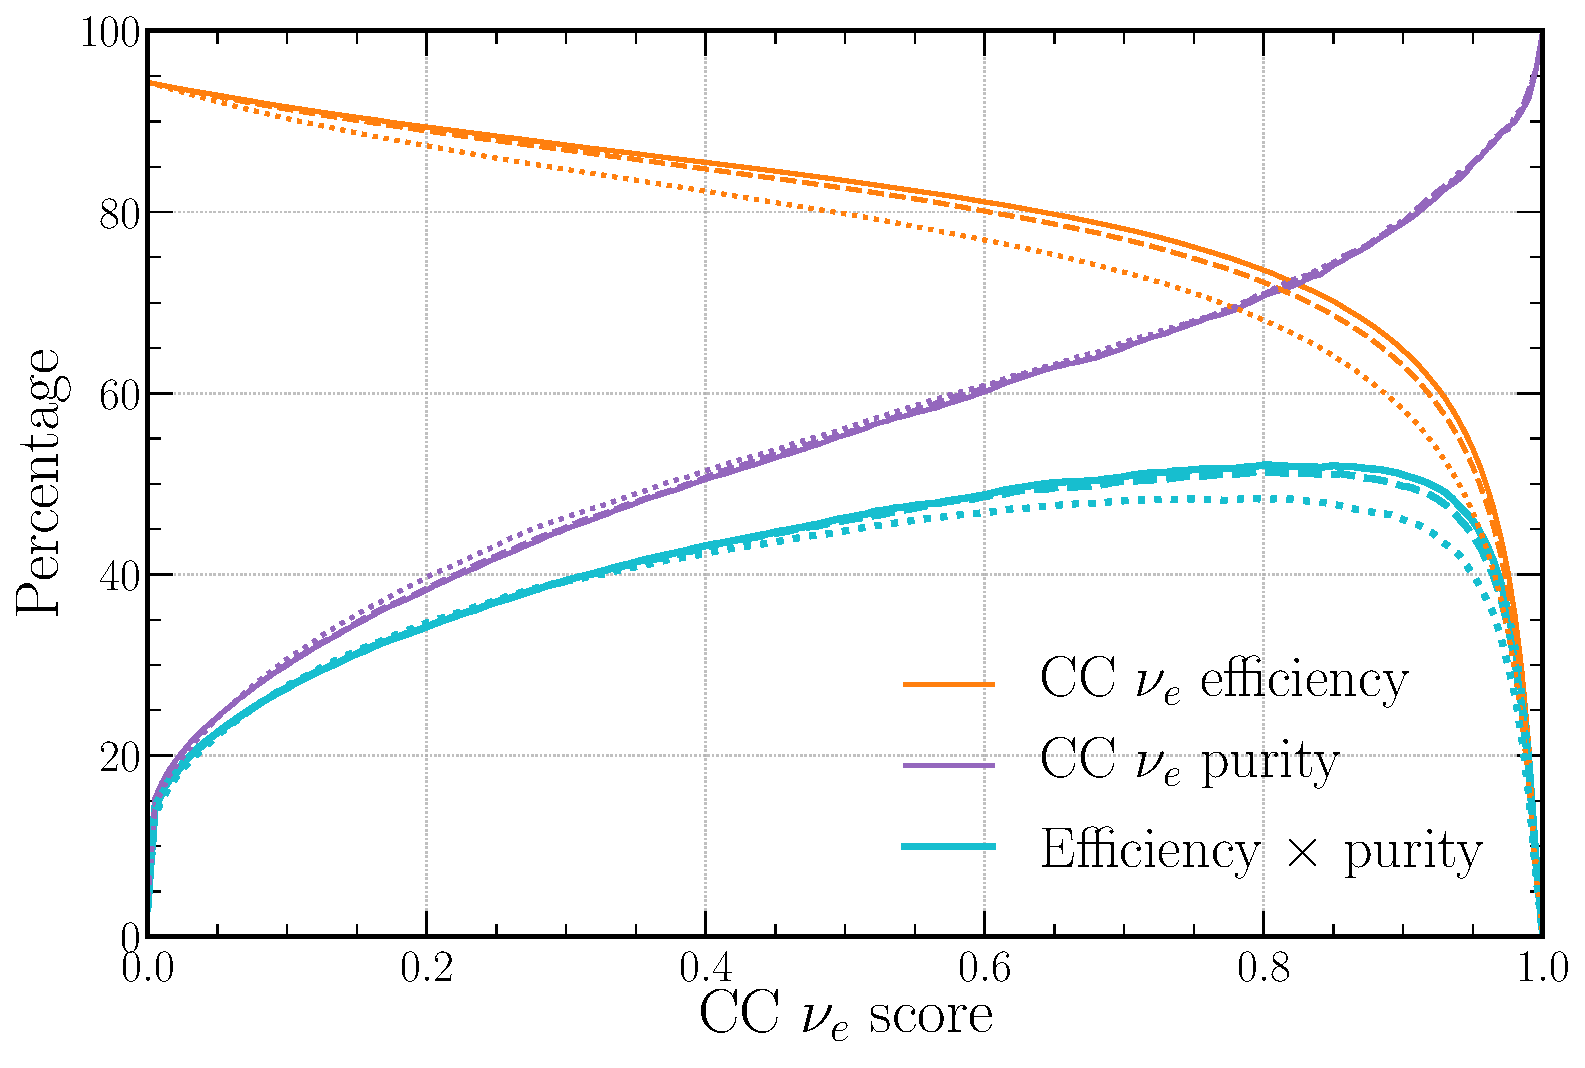
\includegraphics[width=0.7\textwidth]{diagrams/7-results/calib_time_nuel_eff_curves.pdf}
    \caption[CC $\nu_{e}$ efficiency and purity curves for different levels of hit-time smearing]
    {CC $\nu_{e}$ efficiency, purity, and $\text{efficiency}\times\text{purity}$ at different
        values of CC $\nu_{e}$ score selection for different levels of hit-time smearing. The
        $\sigma=0~\text{ns}$ curves are shown by the solid lines, $\sigma=2~\text{ns}$ curves by
        the dashed lines, and $\sigma=5~\text{ns}$ curves by the dotted lines.}
    \label{fig:calib_time_nuel_eff_curves}
\end{figure}

\begin{table} % CALIB TIME COMPARISON METRICS TABLE %
    \begin{tabular}{lrrr}
        Metric         & $\sigma=0~\text{ns}$ & $\sigma=2~\text{ns}$ & $\sigma=5~\text{ns}$ \\
        \midrule
        Max FOM        & \textbf{0.519}       & 0.513                & 0.484                \\
        High Score Eff & \textbf{0.835}       & 0.826                & 0.798                \\
        High Score Pur & 0.554                & 0.556                & \textbf{0.561}       \\
        ROC Integral   & \textbf{0.828}       & 0.828                & 0.826                \\
        PR Integral    & \textbf{0.756}       & 0.751                & 0.730                \\
    \end{tabular}
    \caption[Classification performance metrics for different levels of hit-time smearing]
    {Classification performance metrics for different levels of hit-time smearing. The ROC and PR
        integrals are taken from under the curves shown in
        \FigureRef{fig:calib_time_nuel_comp_curves}.}
    \label{tab:calib_time}
\end{table}

\begin{figure} % CALIB TIME NUEL COMP CURVES DIAGRAM %
    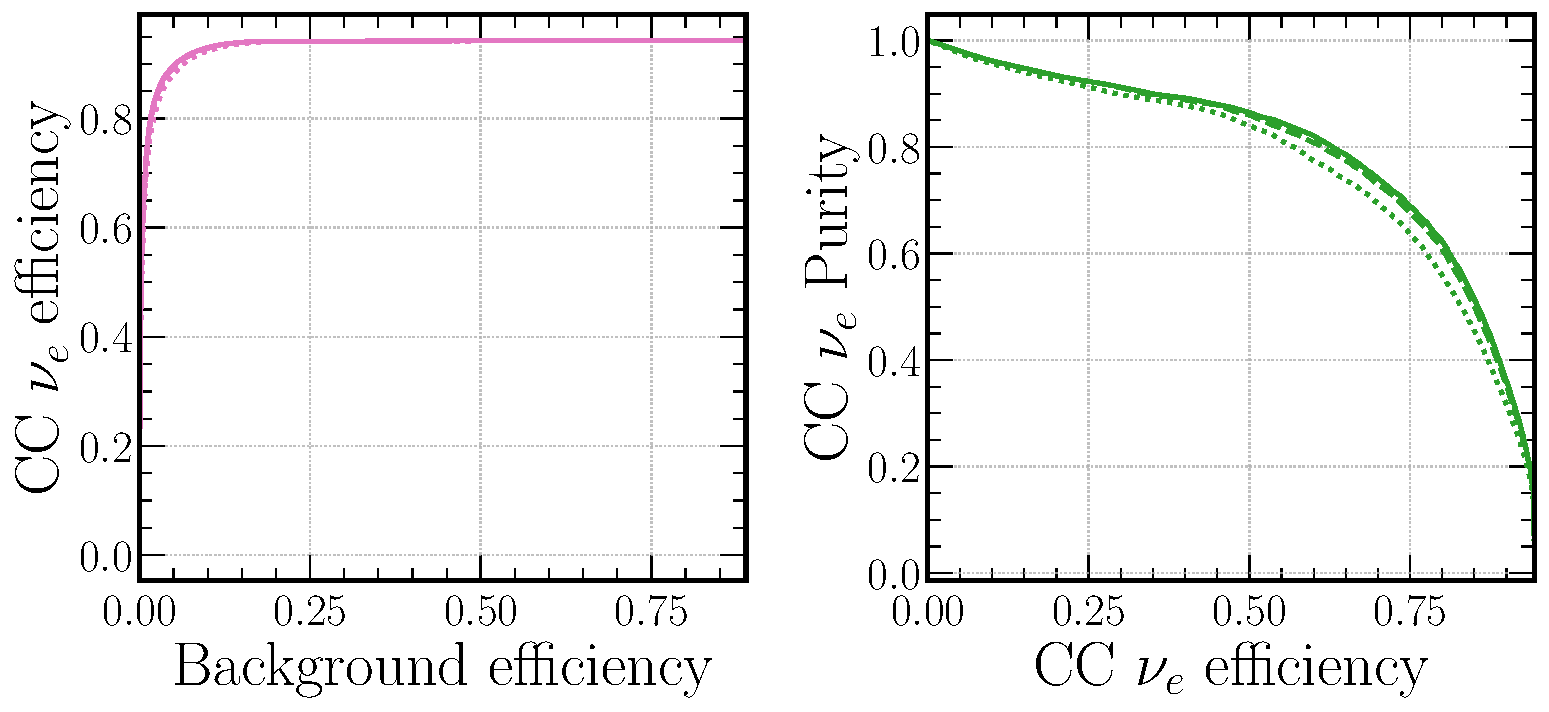
\includegraphics[width=0.9\textwidth]{diagrams/7-results/calib_time_nuel_comp_curves.pdf}
    \caption[Receiver operating characteristic and precision-recall curves for different levels of
        hit-time smearing] {ROC (left) and PR (right) curves for different levels of hit-time
        smearing. The $\sigma=0~\text{ns}$ curves are shown by the solid lines,
        $\sigma=2~\text{ns}$ curves by the dashed lines, and $\sigma=5~\text{ns}$ curves by the
        dotted lines.}
    \label{fig:calib_time_nuel_comp_curves}
\end{figure}

With an effective calibration, a realistic discrepancy in hit times of less than
\unit{1}{\text{ns}} should be expected. Given this, it is promising to observe that even for the
smearing of $\sigma=2~\text{ns}$ the beam classification performance change is minimal. At
$\sigma=5~\text{ns}$ more significant degradation starts to occur; however, there is no dramatic
fall-off in performance. Interestingly, the \emph{High Score Pur} is seen to increase with greater
hit-time smearing, indicating that CC $\nu_{e}$ signal events are proportionally more robust to
hit-time input smearing than background events.

\subsection{Charge smearing and shifting} %%%%%%%%%%%%%%%%%%%%%%%%%%%%%%%%%%%%%%%%%%%%%%%%%%%%%%%%
\label{sec:results_robust_charge} %%%%%%%%%%%%%%%%%%%%%%%%%%%%%%%%%%%%%%%%%%%%%%%%%%%%%%%%%%%%%%%%

The smearing and shifting of input hit charges behave as expected and produce no significant
reduction in output performance. For every event, each hit-charge and hough-height bin is scaled
by a factor randomly drawn from a normal distribution with a mean of $\mu$ and a standard
deviation of $\sigma$. This methodology differs from the absolute hit-time smearing above by
modifying bins proportional to their charge, instead of using an absolute value. Any post
modification bin values outside the zero to one input range are clipped to the range boundaries.

Alongside the default case when $\mu=1.0$ and $\sigma=0.0$, two smearing and two shifting cases
are considered: $\mu=1.0,\sigma=0.2$ and $\mu=1.0,\sigma=0.4$ for smearing; and
$\mu=1.2,\sigma=0.2$ and $\mu=1.4,\sigma=0.2$ for shifting. Note that for the shifting cases a
standard deviation of $\sigma=0.2$ is used to introduce some randomness.

For each smearing case, the resulting efficiency, purity, and their product (the FOM) for CC
$\nu_{e}$ events as a function of selecting events above a particular CC $\nu_{e}$ score is shown
in \FigureRef{fig:calib_charge_rand_nuel_eff_curves}. The equivalent plot for each shifting case
is shown in \FigureRef{fig:calib_charge_shift_nuel_eff_curves}. The classification performance
metrics are presented in \TableRef{tab:calib_charge}, with distributions of (reco-true)/true CC
QEL $\nu_{e}$ energies for each case also shown in \FigureRef{fig:calib_charge_energy}. Cosmic
rejection performance is not presented as the resulting output changes are negligible.

\begin{figure} % CALIB CHARGE RAND NUEL EFF CURVES DIAGRAM %
    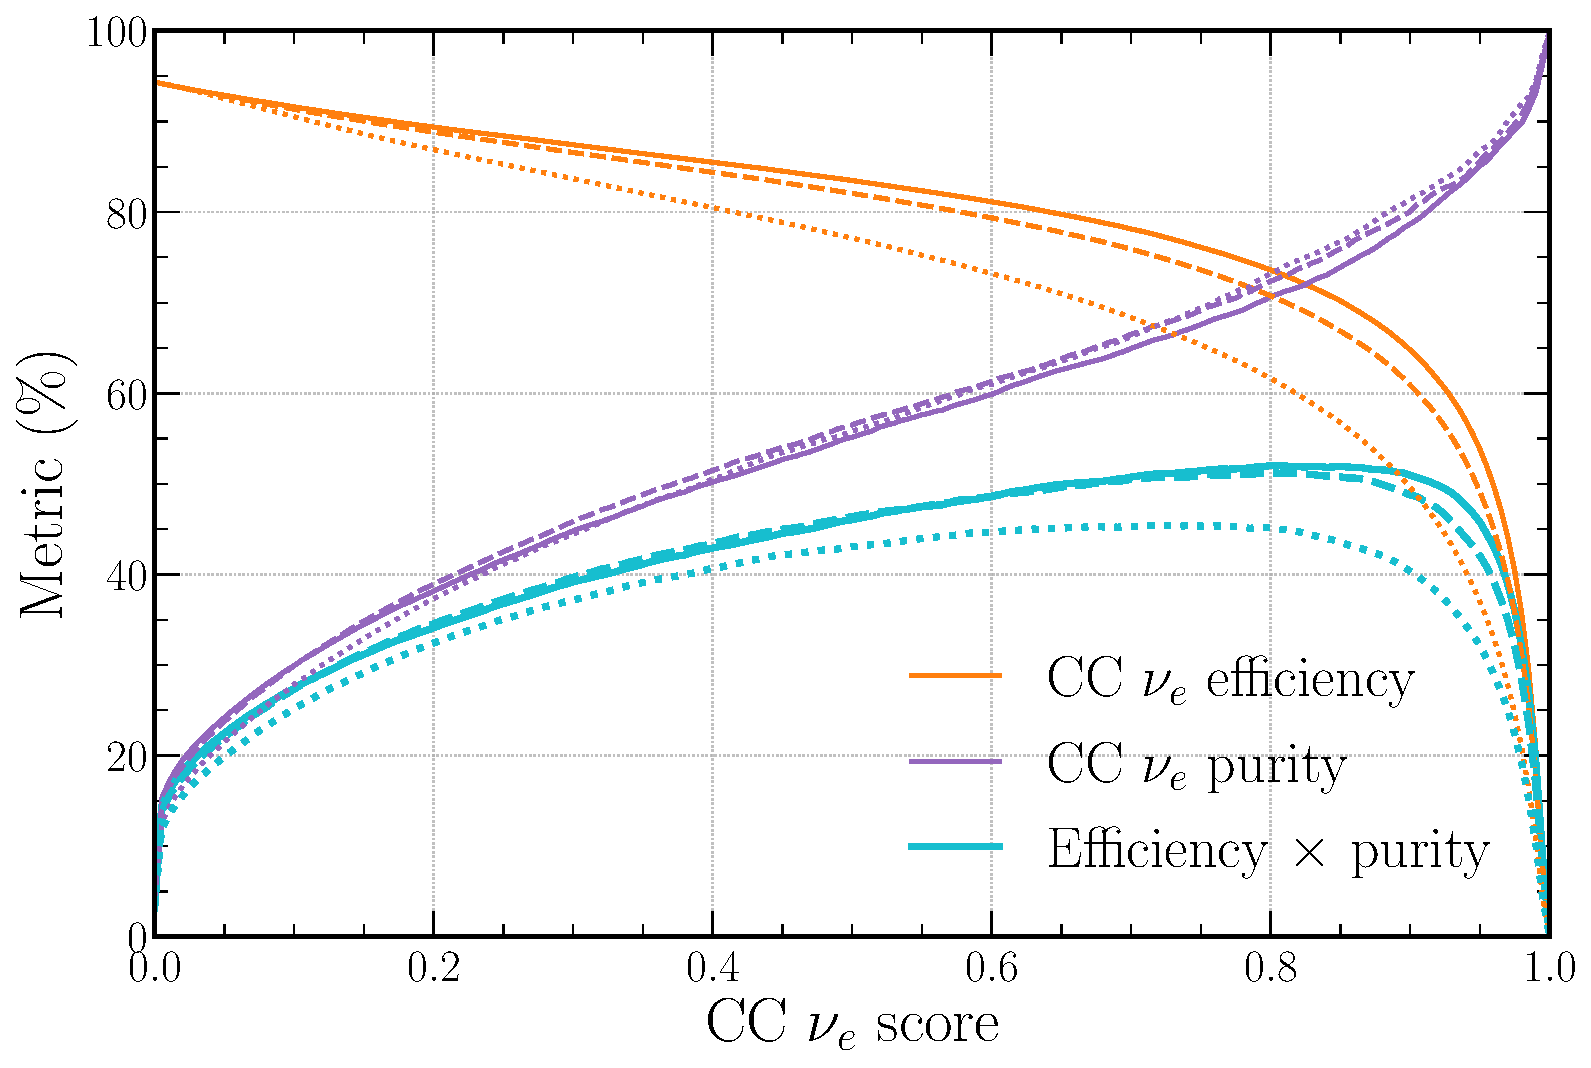
\includegraphics[width=0.7\textwidth]{diagrams/7-results/calib_charge_rand_nuel_eff_curves.pdf}
    \caption[CC $\nu_{e}$ efficiency and purity curves for different levels of hit-charge smearing]
    {CC $\nu_{e}$ efficiency, purity, and $\text{efficiency}\times\text{purity}$ curves at
        different values of CC $\nu_{e}$ score selection for different levels of hit-charge
        smearing where $\mu=1.0$. The $\sigma=0.0$ curves are shown by the solid lines,
        $\sigma=0.2$ curves by the dashed lines, and $\sigma=0.4$ curves by the dotted lines.}
    \label{fig:calib_charge_rand_nuel_eff_curves}
\end{figure}

\begin{figure} % CALIB CHARGE SHIFT NUEL EFF CURVES DIAGRAM %
    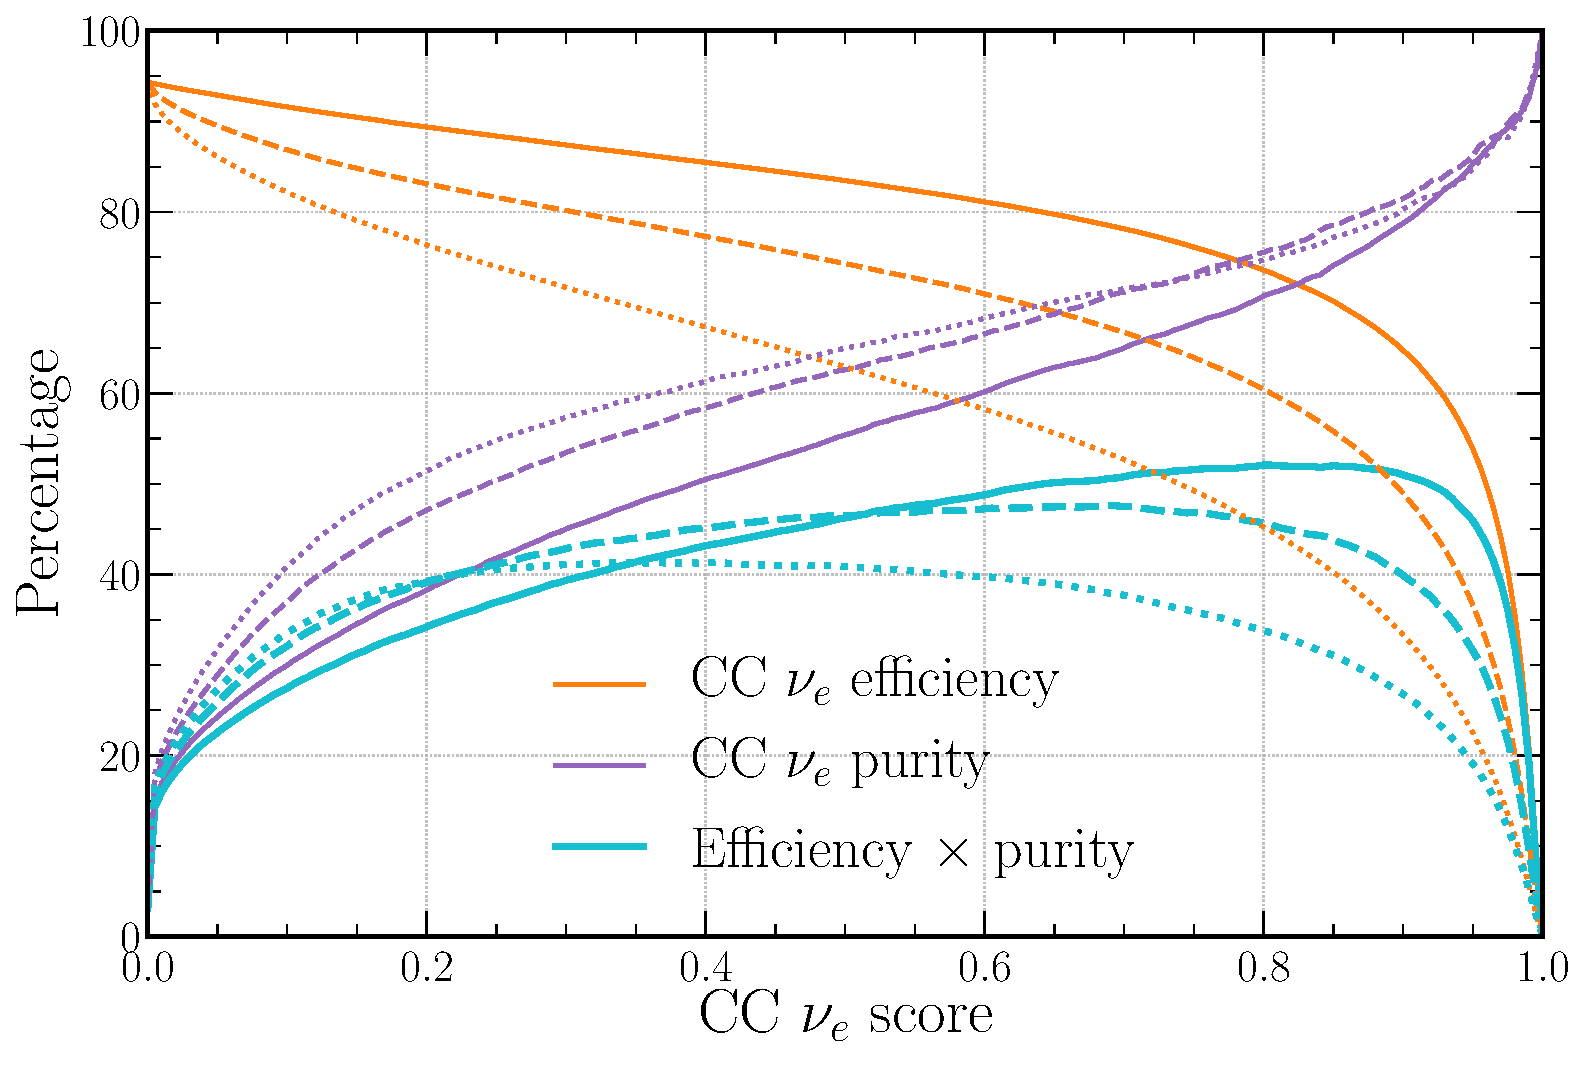
\includegraphics[width=0.7\textwidth]{diagrams/7-results/calib_charge_shift_nuel_eff_curves.pdf}
    \caption[CC $\nu_{e}$ efficiency and purity curves for different levels of hit-charge shifting]
    {CC $\nu_{e}$ efficiency, purity, and $\text{efficiency}\times\text{purity}$ curves at
        different values of CC $\nu_{e}$ score selection for different levels of hit-charge
        shifting. The $\mu=1.0$ curves are shown by the solid lines, $\mu=1.2$ curves by the
        dashed lines, and $\mu=1.4$ curves by the dotted lines.}
    \label{fig:calib_charge_shift_nuel_eff_curves}
\end{figure}

\begin{table} % CALIB CHARGE COMPARISON METRICS TABLE %
    \begin{tabular}{lrrrrr}
        Scaling ($\mu,\sigma$) & ($1.0,0.0$)    & ($1.0,0.2$)    & ($1.0,0.4$) & ($1.2,0.2$) &
        ($1.4,0.2$) \\
        \midrule
        Max FOM                & \textbf{0.519} & 0.513          & 0.458       & 0.519       &
        0.501       \\
        High Score Eff         & \textbf{0.835} & 0.820          & 0.771       & 0.829       &
        0.821       \\
        High Score Pur         & 0.554          & \textbf{0.565} & 0.560       & 0.551       &
        0.532       \\
        ROC Integral           & \textbf{0.828} & 0.828          & 0.825       & 0.827       &
        0.825       \\
        PR Integral            & \textbf{0.756} & 0.751          & 0.707       & 0.750       &
        0.733       \\
    \end{tabular}
    \caption[Classification performance metrics for different levels of hit-charge smearing and
        shifting] {Classification performance metrics for different levels of hit-charge smearing
        and shifting.}
    \label{tab:calib_charge}
\end{table}

\begin{figure} % CALIB CHARGE ABS ENERGY DIAGRAM %
    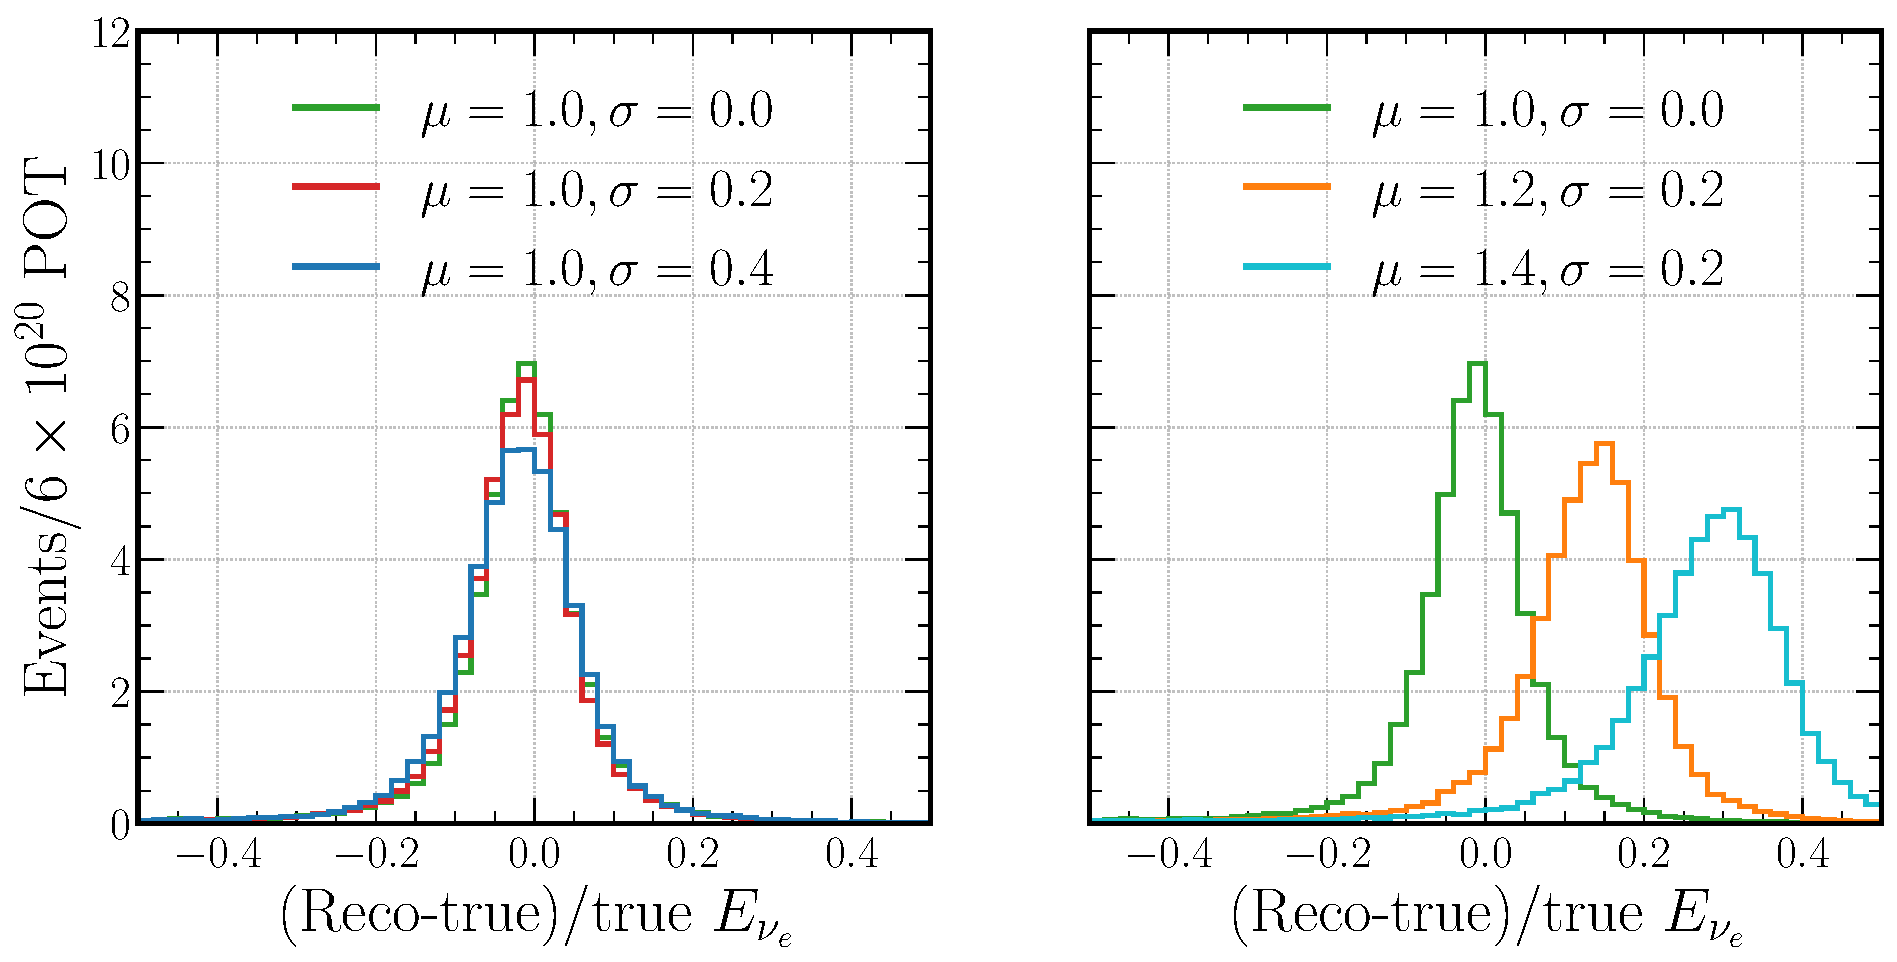
\includegraphics[width=0.9\textwidth]{diagrams/7-results/calib_charge_energy.pdf}
    \caption[Distributions of (reco-true)/true $\nu_{e}$ energies for different levels of
        hit-charge smearing and shifting] {Distributions of (reco-true)/true CC QEL $\nu_{e}$
        energies for different levels of hit-charge smearing and shifting. Shown are the different
        smearing levels (left) and the different shifting levels (right). Standard deviations
        found from fits made to each distribution are shown in brackets.}
    \label{fig:calib_charge_energy}
\end{figure}

With an effective calibration in the smearing case and reasonable modelling in the shifting case,
it is realistic to assume differences on the order of a few per cent for the hit-charge and
hough-height inputs. Given this, the extensive modifications made here (40\% shifts, for example)
still produce only relatively small reductions in beam classification performance; therefore, a
negligible effect can be assumed. Interestingly, smearing of $\sigma=0.4$ is seen to impact
performance to a greater degree than shifting with $\mu=1.4$. This behaviour can be explained by
the overall relative event topology remaining consistent under a shift compared to when smeared.

For neutrino energy estimation, the impact of smearing is small, but shifting is seen to produce
significant changes. This is understandable when assuming that the energy estimation (even for a
CNN) relies principally on the counting of the deposited charge for each event, as is the case for
most experimental particle physics predictions. Therefore, any systematic shift in the measured
input data is always expected to bias the output prediction heavily. However, for realistic input
differences on the order of a few per cent, only small output changes should be expected here.

\subsection{Random noise} %%%%%%%%%%%%%%%%%%%%%%%%%%%%%%%%%%%%%%%%%%%%%%%%%%%%%%%%%%%%%%%%%%%%%%%%
\label{sec:results_robust_noise} %%%%%%%%%%%%%%%%%%%%%%%%%%%%%%%%%%%%%%%%%%%%%%%%%%%%%%%%%%%%%%%%%

Random PMT noise added to the input is found to have a negligible impact on output performance.
For every event hit-charge bin, a normal distribution with a mean of zero and a standard deviation
of $\mu$ photoelectrons is randomly sampled. If a value greater than that corresponding to a
single photoelectron is returned, the bin charge is incremented by the returned value.
Furthermore, for each modification made, the corresponding hit-time bin is updated by randomly
sampling a uniform time distribution and choosing the earliest of the return value and the already
set bin time. Alongside the default case with no noise ($0.0\%$), values of $\mu$ are chosen so
that either $2.3\%$ or $6.7\%$ of bins are modified by random noise in each event.

For each case, the resulting efficiency, purity, and their product (the FOM) for CC $\nu_{e}$
events as a function of selecting events above a particular CC $\nu_{e}$ score is shown in
\FigureRef{fig:calib_noise_nuel_eff_curves}. The classification performance metrics are presented
in \TableRef{tab:calib_noise}. Cosmic rejection and energy estimation performance are not
presented as the resulting output changes are negligible.

\begin{figure} % CALIB NOISE NUEL EFF CURVES DIAGRAM %
    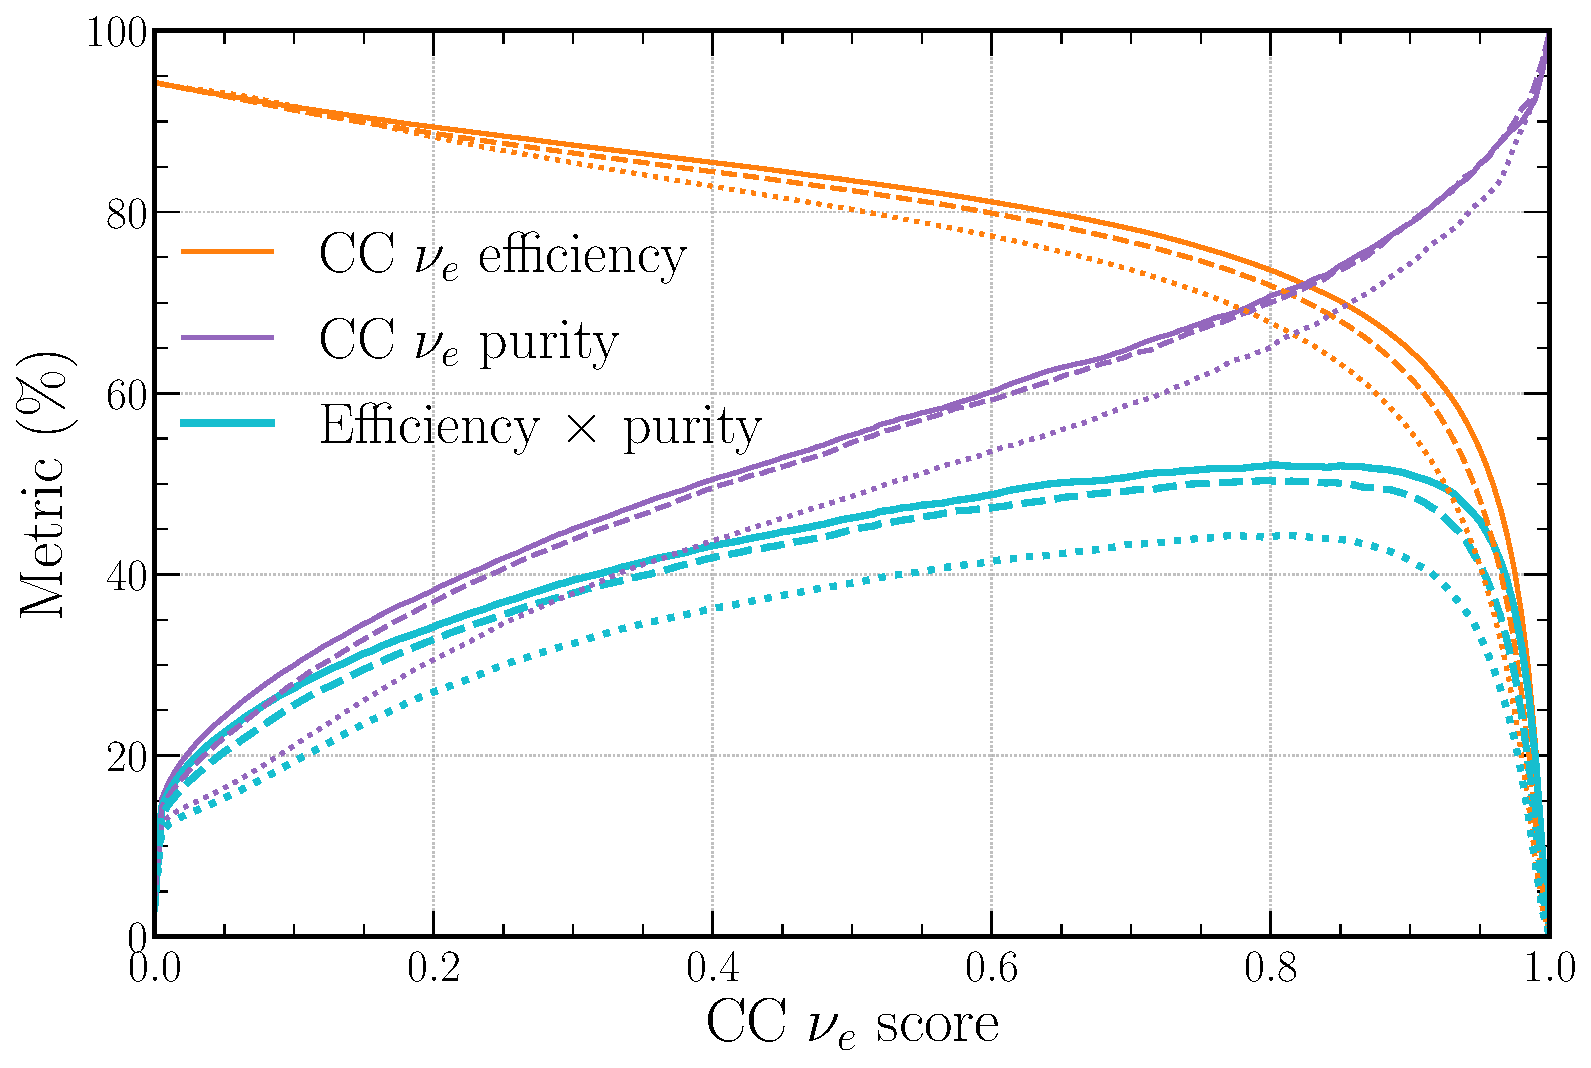
\includegraphics[width=0.7\textwidth]{diagrams/7-results/calib_noise_nuel_eff_curves.pdf}
    \caption[CC $\nu_{e}$ efficiency and purity curves for different levels of random noise]
    {CC $\nu_{e}$ efficiency, purity, and $\text{efficiency}\times\text{purity}$ curves at
        different values of CC $\nu_{e}$ score selection for different levels of random noise. The
        $0.0\%$ curves are shown by the solid lines, $2.3\%$ curves by the dashed lines, and
        $6.7\%$ curves by the dotted lines.}
    \label{fig:calib_noise_nuel_eff_curves}
\end{figure}

\begin{table} % CALIB NOISE COMPARISON METRICS TABLE %
    \begin{tabular}{lrrr}
        Metric         & $0.0\%$        & $2.3\%$ & $6.7\%$ \\
        \midrule
        Max FOM        & \textbf{0.519} & 0.503   & 0.316   \\
        High Score Eff & \textbf{0.835} & 0.824   & 0.717   \\
        High Score Pur & \textbf{0.554} & 0.545   & 0.414   \\
        ROC Integral   & \textbf{0.828} & 0.827   & 0.810   \\
        PR Integral    & \textbf{0.756} & 0.740   & 0.559   \\
    \end{tabular}
    \caption[Classification performance metrics for different levels of random noise]
    {Classification performance metrics for different levels of random noise.}
    \label{tab:calib_noise}
\end{table}

The cases presented here represent a PMT noise rate more than two orders of magnitude greater than
that expected within \chipsfive. Testing has shown that at room temperate the Nikhef \textsc{Pom}
HZC PMTs produce a dark noise rate of $\sim$\unit{1}{\text{KHz}}. Therefore, only $\sim0.02\%$ of
event map bins are expected to be affected by PMT noise throughout a typical \unit{100}{\text{ns}}
event. Given this, excellent beam classification robustness is observed, with the small reduction
in performance seen for the $2.3\%$ chance of noise case indicating any realistic output changes
would be negligible.

\section{Alternative implementations} %%%%%%%%%%%%%%%%%%%%%%%%%%%%%%%%%%%%%%%%%%%%%%%%%%%%%%%%%%%%
\label{sec:results_alt} %%%%%%%%%%%%%%%%%%%%%%%%%%%%%%%%%%%%%%%%%%%%%%%%%%%%%%%%%%%%%%%%%%%%%%%%%%

Here a sample of alternative (but ultimately unsuccessful) \chips CNN implementations are
presented and compared to the final implementation used. Those chosen highlight interesting
factors that are found to drive (or not drive) performance. Only the beam classification
performance, specifically the primary CC $\nu_{e}$ selection is considered here for comparison;
however, these findings also translate to cosmic rejection and energy estimation performance.

\subsection{Alternative inputs} %%%%%%%%%%%%%%%%%%%%%%%%%%%%%%%%%%%%%%%%%%%%%%%%%%%%%%%%%%%%%%%%%%
\label{sec:results_alt_inputs} %%%%%%%%%%%%%%%%%%%%%%%%%%%%%%%%%%%%%%%%%%%%%%%%%%%%%%%%%%%%%%%%%%%

How the raw PMT hits of an event are represented is found to impact performance significantly.
Three different representations are considered. Firstly, the (successful) \emph{vertex view}, were
event maps are generated in $\theta$ and $\phi$ as viewed from the seed estimated interaction
vertex position. Secondly, the \emph{origin raw view}, were event maps are generated in $\theta$
and $\phi$ as viewed from the centre of the detector (the origin). Finally, the \emph{origin iso
view}, were event maps are generated using a PMT position parametrisation in $X_{+}$ and $X_{-}$
as viewed from the centre of the detector.

The origin iso view follows the parametrisation from \ReferenceRef{berns2020}, used for
exploratory Super-Kamiokande (and Hyper-Kamiokande) CNN studies. This mapping attempts to equally
distribute PMT density across the whole two-dimensional input representation. The PMT positions in
cylindrical coordinates ($\rho,\phi,z$) are mapped to two dimensions, $X_{+}$ and $X_{-}$ using
\begin{equation} % ISO CASE EQUATION %
    X_{\pm}=
    \begin{cases}
        1-\chi_{\mp} & (z \geq 0) \\
        \chi_{\pm}   & (z < 0),
    \end{cases}
    \label{eq:iso_case}
\end{equation}
where
\begin{equation} % ISO MAIN EQUATION %
    \chi_{\pm}=W(\rho,z)\frac{\pi\pm\phi}{2\pi},
    \label{eq:iso_main}
\end{equation}
and
\begin{equation} % ISO PART EQUATION %
    W(\rho,z)=\sqrt{\frac{\rho^{2}-2R|z|+RH}{R^{2}+RH}},
    \label{eq:iso_part}
\end{equation}
with $R$ and $H$ being the radius and height of the cylindrical detector respectively.

The same example CC resonant $\nu_{e}$ event for each representation is shown in
\FigureRef{fig:explore_repr_nuel_ccres_event} for reference. The example event highlights the
advantages of representing the event as viewed from its estimated interaction vertex position. The
emitted Cherenkov radiation and resulting ring are viewed without detector or representation
parametrisation distortions, showing their true physical topology. This clarity allows the CNN to
solely learn the underlying topological differences between event types instead of also having to
untangle distortions.

\begin{figure} % EXPLORE REPR EVENT DIAGRAM %
    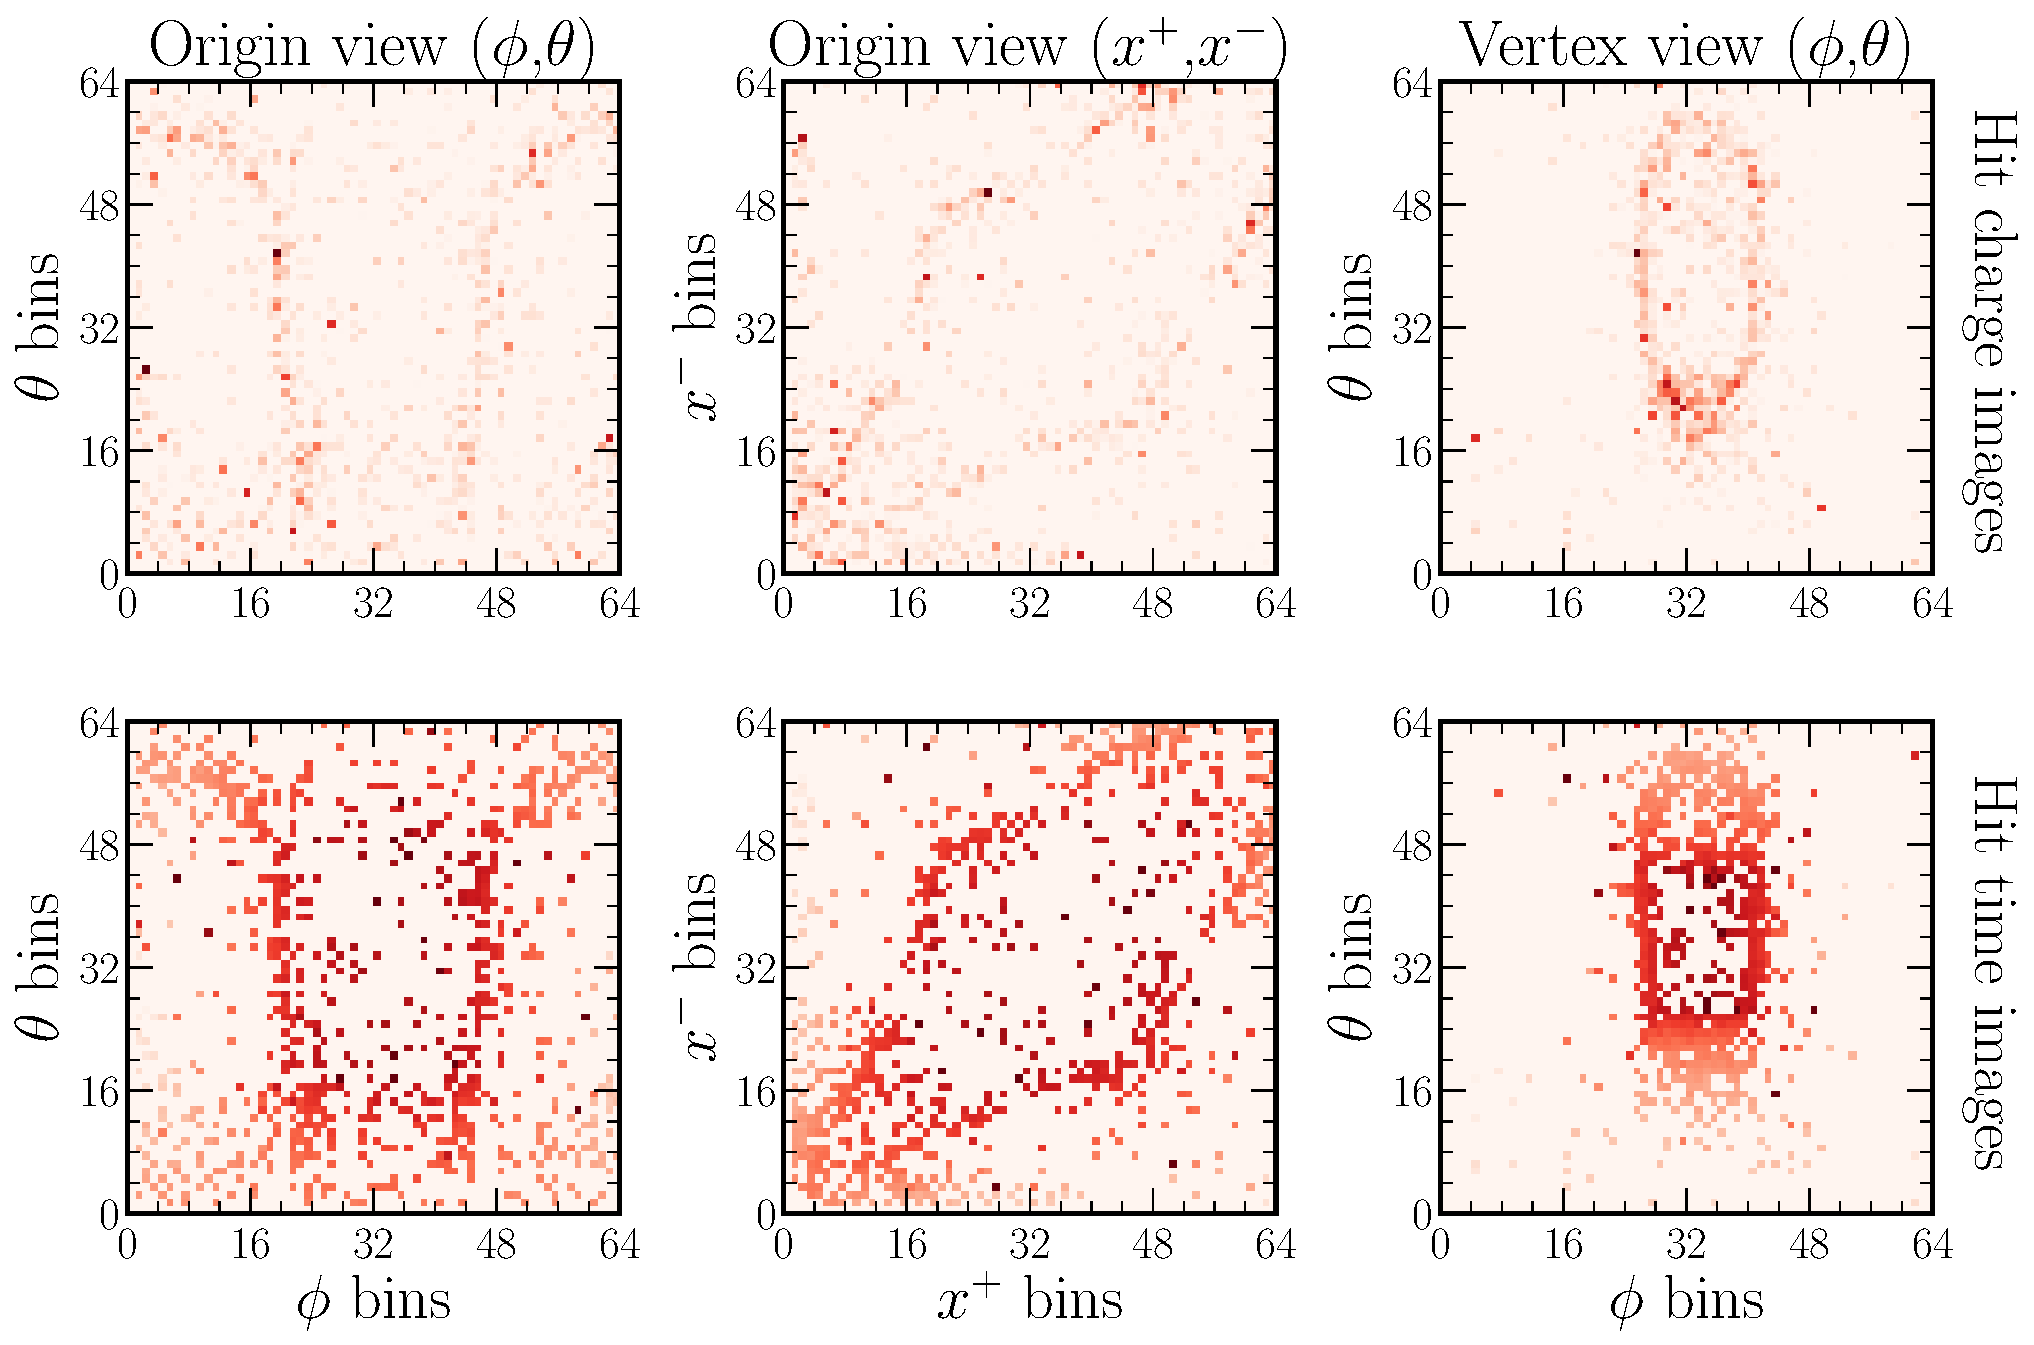
\includegraphics[width=\textwidth]{diagrams/7-results/explore_repr_nuel_ccres_event.pdf}
    \caption[Example CC resonant $\nu_{e}$ event shown for different input representations]
    {Example CC resonant $\nu_{e}$ event shown for each of the three input representations, with
        the hit-charge (top) and hit-time (bottom) event maps shown for each. The event is
        initiated by a $\nu_{e}$ of energy \unit{3.3}{\GeV} with the final state particles above
        the Cherenkov threshold including a $e^{-}$ of energy \unit{2.8}{\GeV} and a
        \unit{0.3}{\GeV} $\pi^{0}$.}
    \label{fig:explore_repr_nuel_ccres_event}
\end{figure}


A beam classification network is trained for each representation. Only the hit-charge and hit-time
event maps are used as input as the hough-height map can only be generated from the seed estimated
interaction vertex position. For each representation the resulting efficiency, purity, and their
product (the FOM) for CC $\nu_{e}$ events as a function of selecting events above a particular CC
$\nu_{e}$ score is shown in \FigureRef{fig:repr_nuel_eff_curves}. Performance comparison metrics
are also presented in \TableRef{tab:repr}.

\begin{figure} % REPR NUEL EFF CURVES DIAGRAM %
    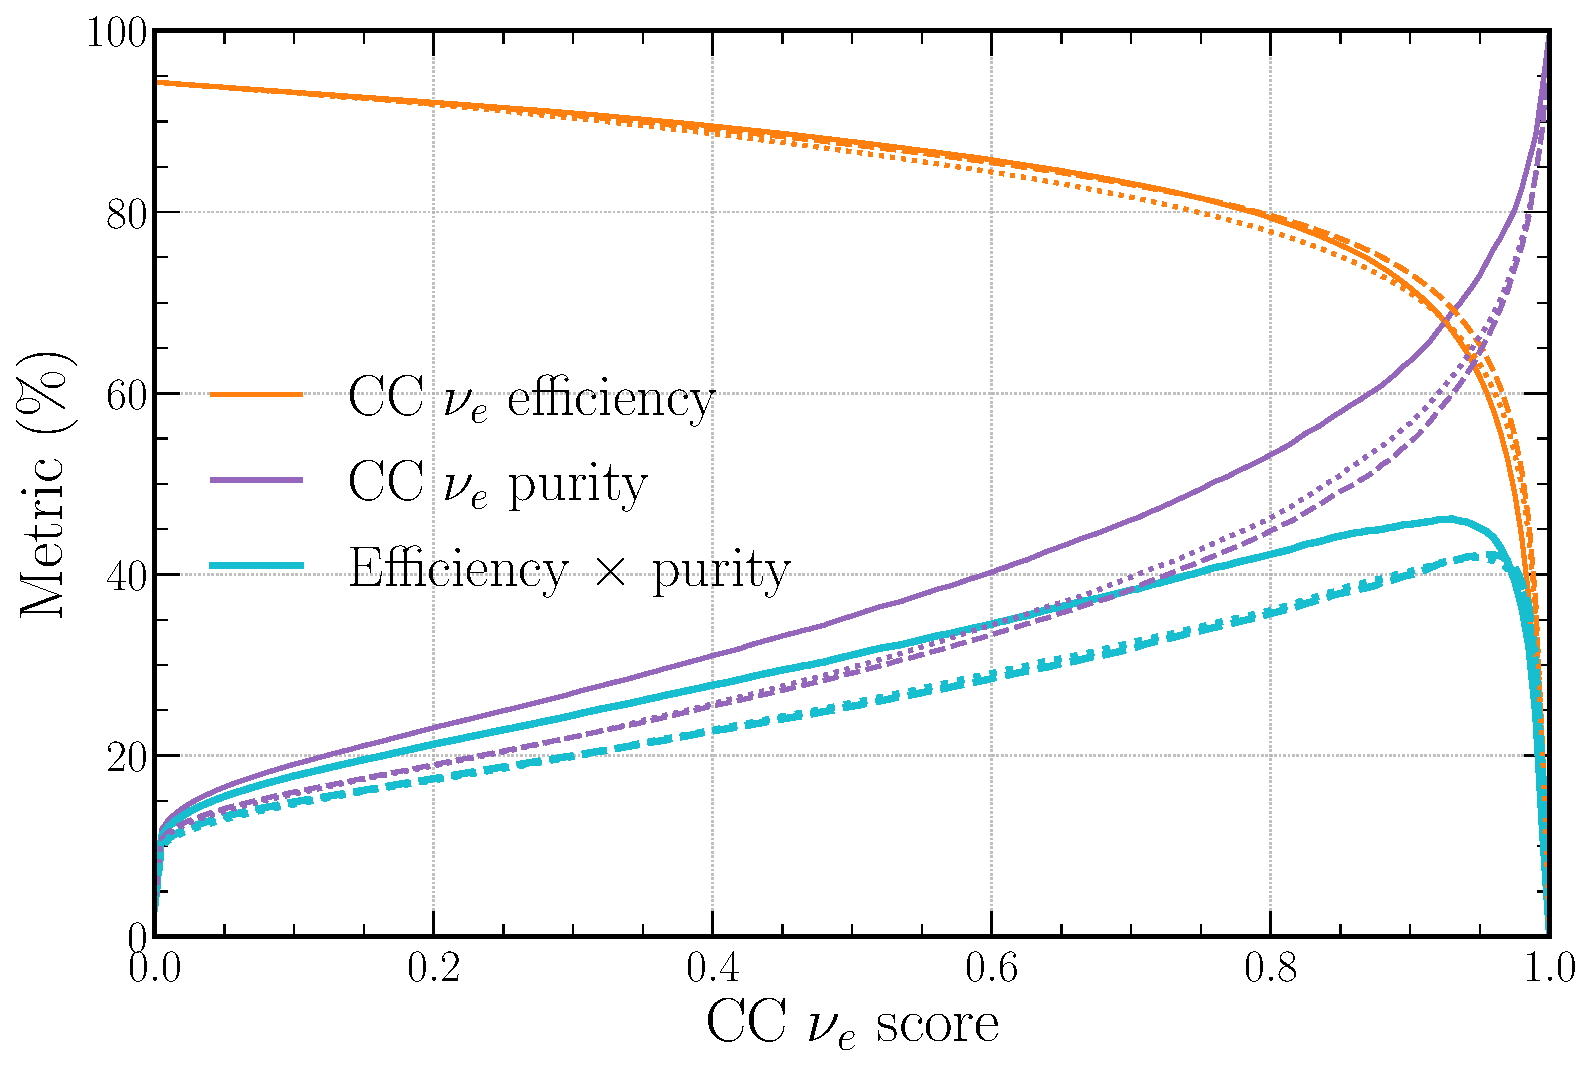
\includegraphics[width=0.7\textwidth]{diagrams/7-results/repr_nuel_eff_curves.pdf}
    \caption[CC $\nu_{e}$ efficiency and purity curves for different input representations]
    {CC $\nu_{e}$ efficiency, purity, and $\text{efficiency}\times\text{purity}$ curves for
        different values of CC $\nu_{e}$ score selection for the three input representations. The
        \emph{vertex view} curves are shown by the solid lines, the \emph{origin raw view} curves
        by the dashed lines, and the \emph{origin iso view} curves by the dotted lines.}
    \label{fig:repr_nuel_eff_curves}
\end{figure}

\begin{table} % REPR COMPARISON METRICS TABLE %
    \begin{tabular}{lrrr}
        Metric         & Vertex View    & Origin Raw View & Origin Iso View \\
        \midrule
        Max FOM        & \textbf{0.461} & 0.422           & 0.419           \\
        High Score Eff & \textbf{0.878} & 0.874           & 0.867           \\
        High Score Pur & \textbf{0.354} & 0.291           & 0.298           \\
        ROC Integral   & \textbf{0.825} & 0.822           & 0.821           \\
        PR Integral    & \textbf{0.707} & 0.675           & 0.670           \\
    \end{tabular}
    \caption[Classification performance metrics for different input representations]
    {Classification performance metrics for the three input representations.}
    \label{tab:repr}
\end{table}

A significant reduction in performance is observed when using either origin view representation,
quantifying the qualitative description using the example event given above. Interestingly, both
origin view representations result in a very similar performance, showing that a uniform PMT
distribution across the input representation does not provide an improvement. Future work should
consider other methods to reduce distortions, such as the smearing of hits across nearby bins to
reduce isolated peaks and an improved interaction vertex position estimation procedure.

\subsection{Alternative training samples} %%%%%%%%%%%%%%%%%%%%%%%%%%%%%%%%%%%%%%%%%%%%%%%%%%%%%%%%
\label{sec:results_samples} %%%%%%%%%%%%%%%%%%%%%%%%%%%%%%%%%%%%%%%%%%%%%%%%%%%%%%%%%%%%%%%%%%%%%%

The relative proportions of training sample interaction types should match the expected sample as
closely as possible. Three different training samples are considered. Firstly, the (successful)
\emph{flux} sample representative of the expected spectrum. Secondly, a \emph{uniform} sample,
using a similar number of events per interaction type as shown in
\FigureRef{fig:explore_uniform_training_sample}. Finally, a \emph{both} sample using an equivalent
combination of both.

\begin{figure} % UNIFORM TRAINING SAMPLE DIAGRAM %
    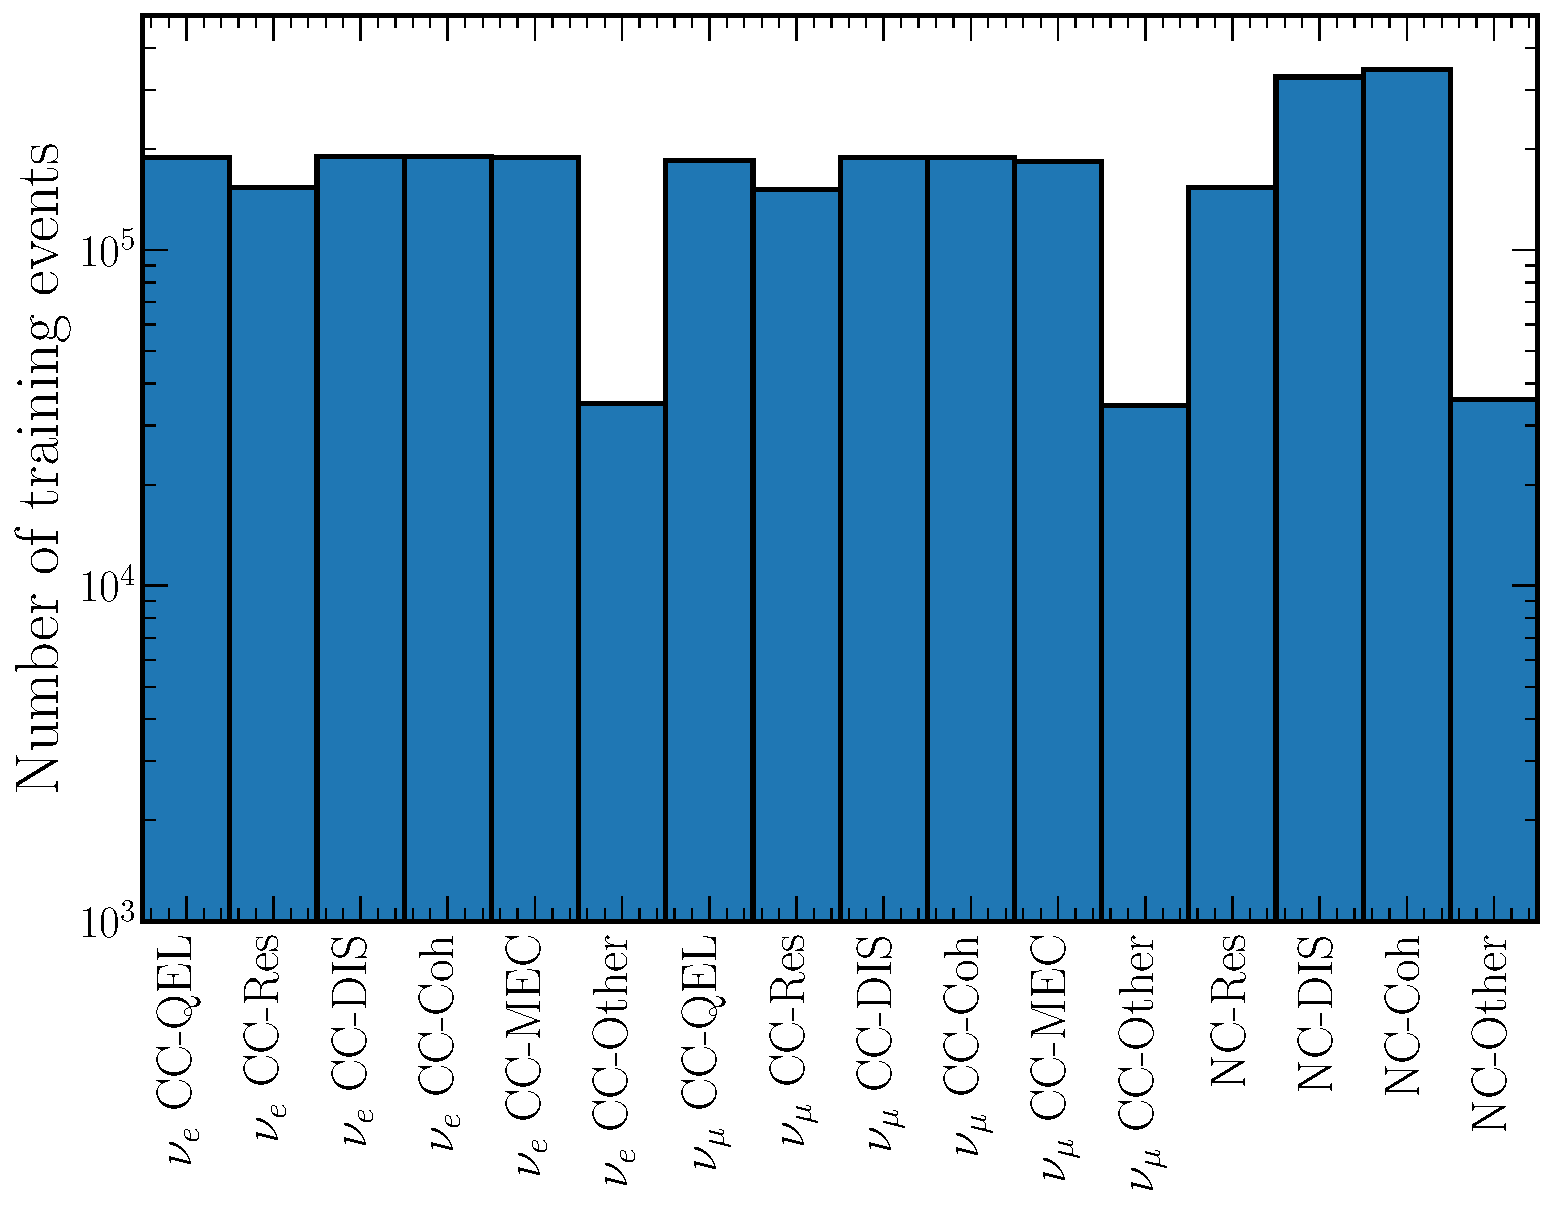
\includegraphics[width=0.7\textwidth]{diagrams/7-results/explore_uniform_training_sample.pdf}
    \caption[Number of training events per category for the uniform beam classification network
        training sample] {Number of training events per category for the uniform beam
        classification network training sample. All beam event interaction types are shown.}
    \label{fig:explore_uniform_training_sample}
\end{figure}

A beam classification network is trained using each of the samples with an equal number of events.
For each sample the resulting efficiency, purity, and their product (the FOM) for CC $\nu_{e}$
events as a function of selecting events above a particular CC $\nu_{e}$ score is shown in
\FigureRef{fig:sample_nuel_eff_curves}. Performance comparison metrics are also presented in
\TableRef{tab:sample}.

\begin{figure} % SAMPLE NUEL EFF CURVES DIAGRAM %
    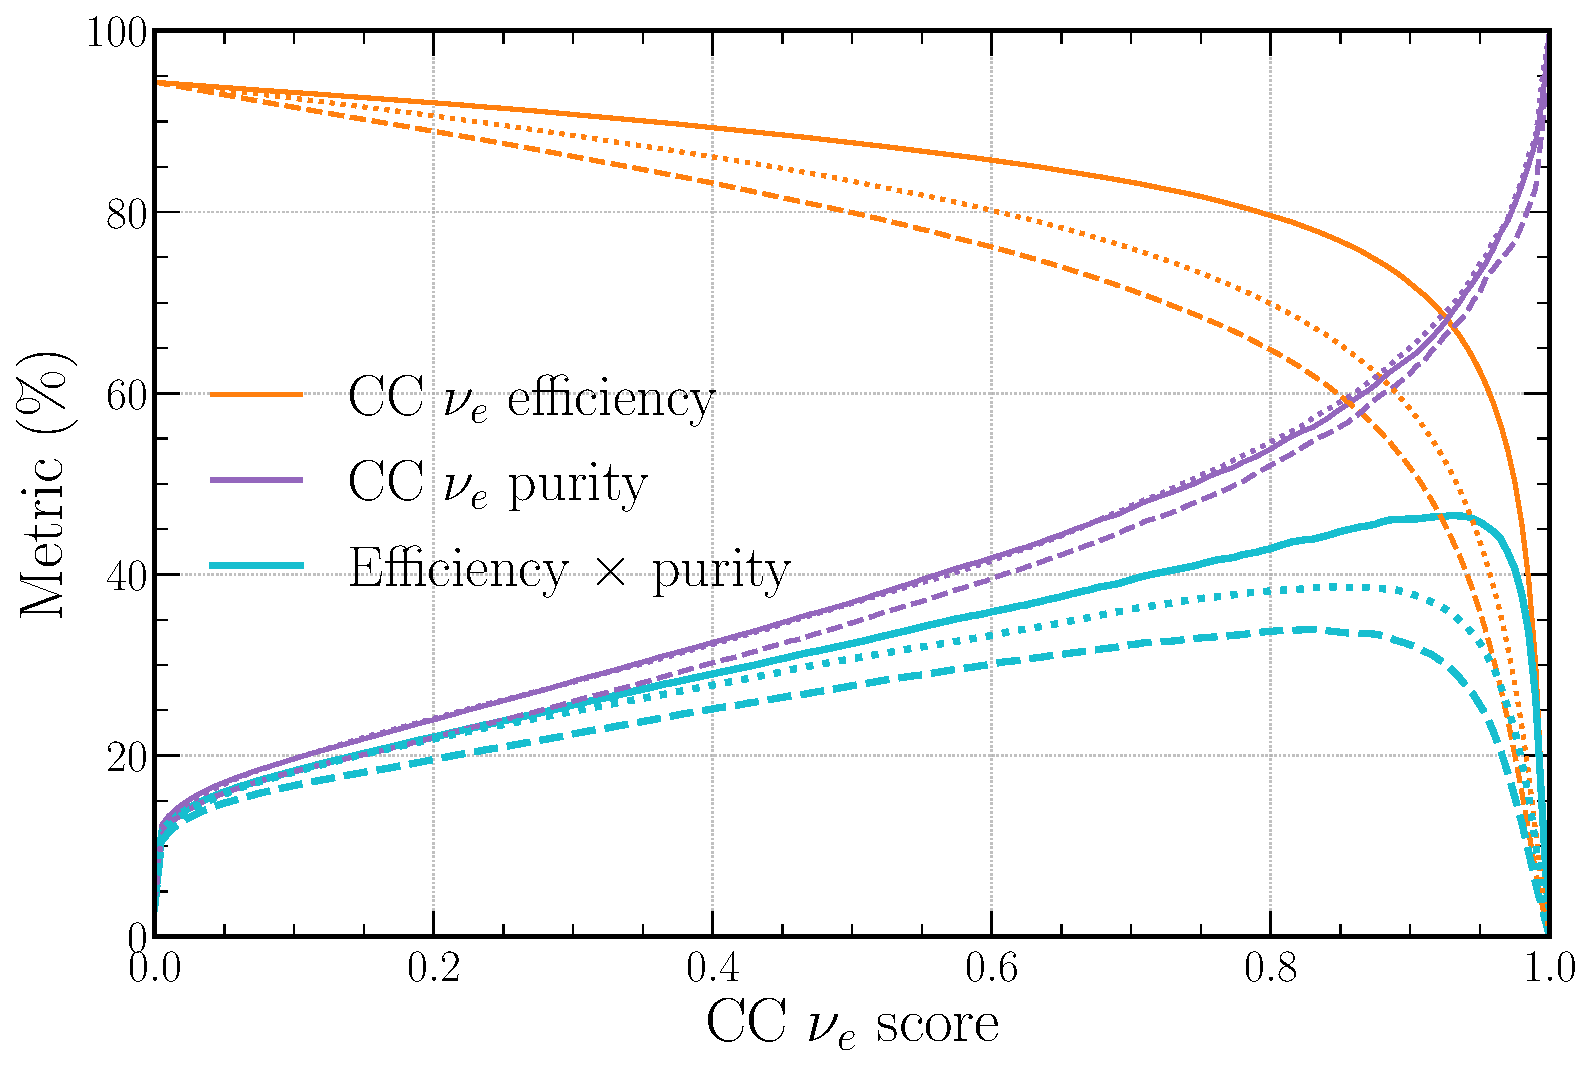
\includegraphics[width=0.7\textwidth]{diagrams/7-results/sample_nuel_eff_curves.pdf}
    \caption[CC $\nu_{e}$ efficiency and purity curves for different training samples]
    {CC $\nu_{e}$ efficiency, purity, and $\text{efficiency}\times\text{purity}$ curves for
        different values of CC $\nu_{e}$ score selection for the different training samples. The
        \emph{flux} sample curves are shown by the solid lines, the \emph{uniform} sample curves
        by the dashed lines, and the \emph{both} curves by the dotted lines.}
    \label{fig:sample_nuel_eff_curves}
\end{figure}

\begin{table} % SAMPLE COMPARISON METRICS TABLE %
    \begin{tabular}{lrrr}
        Metric         & Flux           & Uniform & Both  \\
        \midrule
        Maximum FOM    & \textbf{0.465} & 0.339   & 0.386 \\
        High Score Eff & \textbf{0.877} & 0.799   & 0.834 \\
        High Score Pur & \textbf{0.369} & 0.347   & 0.368 \\
        ROC Integral   & \textbf{0.826} & 0.815   & 0.820 \\
        PR Integral    & \textbf{0.712} & 0.568   & 0.634 \\
    \end{tabular}
    \caption[Classification performance metrics for different training samples]
    {Classification performance metrics for the different training samples.}
    \label{tab:sample}
\end{table}

Using the uniform training sample is found to reduce beam classification performance
significantly. Given that the \emph{both} sample performance lies between the uniform and flux
cases, it can be assumed that as the training sample tends towards the expected distribution of
events, the performance increases. This finding highlights a key feature of CNNs; they play the
game of statistics and only statistics, making them less smart than they may first appear.

In the beam classification case, the CNN learns to minimise the categorical cross-entropy loss
function, maximising the fraction of total training events that are classified correctly. An easy
way to do this is to become heavily biased by the averages of the sample used during training,
such that the final performance does not generalise well to a different evaluation sample.

For the flux training sample case, less common event classes are ignored by the network during
training, as solely focusing on the dominant classes is found to be the easiest way to minimise
the loss. The effect of this can be seen in the interaction type classification matrices in
\SectionRef{sec:results_eval_beam} for CC-Coh and CC-MEC events. Future work should consider the
use of a different loss function to promote learning for the less common interaction types and to
maximise the physics sensitivity rather than majority accuracy.

\subsection{Alternative architectures} %%%%%%%%%%%%%%%%%%%%%%%%%%%%%%%%%%%%%%%%%%%%%%%%%%%%%%%%%%%
\label{sec:results_alt_arch} %%%%%%%%%%%%%%%%%%%%%%%%%%%%%%%%%%%%%%%%%%%%%%%%%%%%%%%%%%%%%%%%%%%%%

The choice of CNN architecture is found to have a minimal impact on performance. Four different
network architectures are considered: the default VGG based chipsnet architecture, an Inception
(GoogLeNet) based architecture~\cite{szegedy2015}, a ResNet based
architecture~\cite{he2016_improved}, and an Inception-ResNet based
architecture~\cite{szegedy2016}. Each is modified to fit the standard chipsnet pattern with
separate initial branches for each event map followed by a series of combined layers. For a fair
comparison, each network is scaled so that they all have approximately the same number of
trainable parameters as the default VGG based architecture.

A beam classification network is trained using each network architecture with individually
optimised hyperparameters (using SHERPA). For each network architecture, the classification
performance metrics are presented in \TableRef{tab:arch} along with the number of trainable
parameters (Number of pars) and the time taken in milliseconds to complete a single training
iteration step (Iter time).

\begin{table} % ARCHITECTURE COMPARISON METRICS TABLE %
    \begin{tabular}{lrrrr}
        Metric         & VGG            & Inception  & ResNet              & Inception-ResNet \\
        \midrule
        Number of pars & 17,225,296     & 16,893,216 & \textbf{16,526,288} & 17,145,238       \\
        Iter time (ms) & \textbf{88}    & 192        & 112                 & 209              \\
        Maximum FOM    & \textbf{0.465} & 0.459      & 0.445               & 0.444            \\
        High Score Eff & \textbf{0.877} & 0.870      & 0.869               & 0.874            \\
        High Score Pur & 0.369          & 0.373      & \textbf{0.374}      & 0.349            \\
        ROC Integral   & \textbf{0.825} & 0.825      & 0.824               & 0.824            \\
        PR Integral    & \textbf{0.712} & 0.706      & 0.688               & 0.699            \\
    \end{tabular}
    \caption[Classification performance metrics for different network architectures]
    {Classification performance metrics for the different network architectures.}
    \label{tab:arch}
\end{table}

Only small performance differences are observed across the different CNN architectures, with the
simplest and least modern, the VGG architecture, proving the highest performing. Furthermore, the
VGG architecture provides the fastest training step iteration time by a significant margin,
leading to drastically lower overall training times.

The other architectures are primarily the result of advances aimed at improving the classification
of real-world objects, such as cars, trees, and dogs, with image sizes typically $256\times256$
pixels or greater. Therefore, it is likely that the task of learning subtle changes in Cherenkov
ring topologies, with a relatively limited number of classes, on small $64\times64$ images, does
not require the advanced feature representation they provide. Using the increased complexity
models instead introduces additional bias, acting to decrease performance instead of providing
additional discriminating power.